\documentclass[11pt, titlepage, bibliography=totoc]{scrreprt}
\setcounter{tocdepth}{3}

\usepackage[a4paper, hmargin=2.5cm, vmargin=3cm]{geometry}
\usepackage[T1]{fontenc}
\usepackage{setspace}
% remove indentation
\setlength{\parindent}{0pt}   
% add spacing between paragraphs
\setlength{\parskip}{1em}     
\usepackage{lmodern}
\usepackage[utf8]{inputenc}
\usepackage[english]{babel}
\usepackage{microtype}
\usepackage{csquotes}

\usepackage{amsmath}
\usepackage{blkarray}
\usepackage{tikz}
\usepackage{booktabs}
\usepackage{tabularx}
\usepackage{pgfplots}
\usepackage{graphicx}
\usepackage{caption, ragged2e}
\usepackage{subcaption}
\usepackage{multirow}
\usepackage{float}
\usepackage{empheq}
\usepackage{amssymb, amsthm}
\usepackage[automark]{scrlayer-scrpage}
\usepackage{listings}
\usepackage{scrhack}
\usepackage[linesnumbered,ruled,vlined]{algorithm2e}
\usepackage{comment}
% needed for \color in listings
\usepackage{xcolor} 
\usepackage{hyperref}

\hypersetup{
    colorlinks=true,
    linkcolor=blue,
    citecolor=blue,
    urlcolor=blue,
    pdftitle={Categorizing Incident Reports Using Traditional Machine Learning and Large Language Models},
    pdfauthor={Md Shariar Imroze Khan},
    pdfsubject={Master Thesis - University of Koblenz},
    pdfkeywords={Process Safety, Incident Classification, Machine Learning, NLP, BERT, LLM}
}

\thispagestyle{empty}

\usetikzlibrary{automata, positioning, arrows, intersections}
\pgfplotsset{compat=1.18}

\newcommand{\matindex}[1]{\mbox{\scriptsize#1}}
\newcolumntype{L}{>{\RaggedRight\arraybackslash}X}

\pagestyle{scrheadings}
\setkomafont{disposition}{\normalfont\bfseries}
\clearpairofpagestyles
\ohead{\headmark}
\ofoot*{\pagemark}

\lstset{
    language=Python,
    basicstyle=\ttfamily\small,
    keywordstyle=\color{blue},
    stringstyle=\color{red},
    commentstyle=\color{green},
    morecomment=[l][\color{magenta}]{\#},
    columns=fullflexible,
    breaklines=true,
    breakatwhitespace=true,
}

\usepackage[style=numeric,sorting=none,maxbibnames=4]{biblatex}
\addbibresource{Literature.bib}

\begin{document}

\begin{titlepage}
\newcommand{\trtitle}{Categorizing Incident Reports Using Traditional Machine Learning and Large Language Models: A Comparative Study}
\newcommand{\trtype}{Master Thesis}
\newcommand{\trdate}{Winter Term 2025/26, \today}
\newcommand{\trauthor}{Md Shariar Imroze Khan (Matriculation No: 220202354)}

\newcommand{\trInstitute}{in the program \\ M. Sc. Mathematical Modelling, Simulation and Optimization \vspace{1em}}
\newcommand{\trUniversity}{Faculty 3: Mathematics / Natural Sciences\\ University of Koblenz}

\begin{flushright}
\includegraphics[height=50pt]{Images/uniLogo.pdf}
\end{flushright}
\vspace{2.5cm}
\begin{center}
  \textbf{\Huge \trtitle}
\end{center}
\vspace{2cm}

\begin{center}
        \textbf{\Large \trtype}\\[1em]
        \trInstitute \\
        \trUniversity \\[1em]
    Submitted by \\[1em]
        \textbf{\large \trauthor}
   
  \vspace{2em}
  \trdate \\ [4em]
  \begin{tabular}{rl}
    First Supervisor: & Prof. Dr. Andreas Mauthe\\
                & {\footnotesize Institut für Wirtschafts- und Verwaltungsinformatik}\\
                & {\footnotesize FG IT Security and Data Security}\\[0.8em]
    Second Supervisor: & Alexander Rosenbaum\\
                & {\footnotesize Institut für Wirtschafts- und Verwaltungsinformatik}\\
                & {\footnotesize FG IT Security and Data Security}\\[0.8em]
    Company Supervisor: & Dr. Hugh Burnham-Slipper\\
                & {\footnotesize Uniper Kraftwerke GmbH}\\
\end{tabular}

\end{center}
\vspace{1cm}
\vfill

\end{titlepage}

\chapter*{Abstract}
\addcontentsline{toc}{chapter}{Abstract}

Incident reporting is a critical process for maintaining safety and operational efficiency across industries such as energy, mining, and healthcare. However, manual classification of incident reports remains prone to human error, inconsistency, and inefficiency. This thesis investigates the application of machine learning and large language models (LLMs) for automated classification of process safety incidents in multilingual industrial datasets.

A comprehensive experimental framework was developed through eight iterative phases, progressively advancing from a controlled BERT-based baseline with Support Vector Machines to more sophisticated multilingual transformer and LLM-based approaches. The research evaluates traditional machine learning approaches (SVM, Random Forest, XGBoost, LightGBM) against transformer-based models (BERT, RoBERTa, DeBERTa, multilingual variants) across four language-specific datasets, including English, German, Swedish, and Dutch incident reports derived from a harmonised master dataset.

Key contributions include a detailed preprocessing pipeline for multilingual incident data, comparative benchmarking of more than 10 transformer architectures, advanced class balancing strategies including SMOTE and language-aware undersampling, ensemble methods combining multiple classifiers, and LLM-based few-shot classification using Flan-T5 models.

Experimental results show that Iteration~0 compared three alternative English subset construction strategies under a common BERT-base-uncased embedding pipeline with feature standardisation and an RBF-kernel SVM classifier. The manually curated English subset was retained as the official baseline and achieved an accuracy of 0.8112 and a macro F1-score of 0.7825. The automatically constructed Lingua-based and langdetect-based subsets achieved macro F1-scores of 0.7758 and 0.7914, respectively. Although the langdetect subset yielded the strongest automatic-subset performance, the manually curated English subset was retained as the official baseline because it provides the most controlled and auditable reference point for subsequent comparisons. Building on this baseline, later iterations improved performance through multilingual embeddings, stronger transformer architectures, and advanced machine learning techniques. The study addresses four research questions concerning classification accuracy improvements, traditional ML versus LLM comparisons, hazard type extraction, and a comprehensive severity prediction framework for the business case.


\cleardoublepage

\chapter*{Zusammenfassung}
\addcontentsline{toc}{chapter}{Zusammenfassung}

Die Meldung von Vorfällen ist ein zentraler Prozess zur Gewährleistung von Sicherheit und betrieblicher Effizienz in Branchen wie der Energieversorgung, dem Bergbau und dem Gesundheitswesen. Die manuelle Klassifikation von Vorfallsberichten ist jedoch weiterhin anfällig für menschliche Fehler, Inkonsistenzen und Ineffizienz. Diese Arbeit untersucht den Einsatz von Machine Learning und Large Language Models (LLMs) zur automatisierten Klassifikation von Process-Safety-Vorfällen in mehrsprachigen industriellen Datensätzen.

Im Rahmen der Untersuchung wurde ein umfassendes experimentelles Framework in acht iterativen Phasen entwickelt, das sich schrittweise von einer kontrollierten BERT-basierten Baseline mit Support Vector Machines hin zu anspruchsvolleren mehrsprachigen Transformer- und LLM-basierten Ansätzen weiterentwickelte. Die Forschung vergleicht traditionelle Machine-Learning-Ansätze (SVM, Random Forest, XGBoost, LightGBM) mit transformerbasierten Modellen (BERT, RoBERTa, DeBERTa sowie mehrsprachigen Varianten) auf vier sprachspezifischen Datensätzen mit englischen, deutschen, schwedischen und niederländischen Vorfallsberichten, die aus einem harmonisierten Master-Datensatz abgeleitet wurden.

Zu den zentralen Beiträgen gehören eine detaillierte Vorverarbeitungspipeline für mehrsprachige Vorfallsdaten, ein vergleichendes Benchmarking von mehr als 10 Transformer-Architekturen, fortgeschrittene Strategien zum Klassen-Balancing einschließlich SMOTE und sprachbewusstem Undersampling, Ensemble-Methoden zur Kombination mehrerer Klassifikatoren sowie eine LLM-basierte Few-Shot-Klassifikation unter Verwendung von Flan-T5-Modellen.

Die experimentellen Ergebnisse zeigen, dass in Iteration~0 drei alternative Strategien zur Bildung englischsprachiger Teilmengen unter einer gemeinsamen Pipeline aus BERT-base-uncased-Embeddings, Merkmalsstandardisierung und einem SVM-Klassifikator mit RBF-Kernel verglichen wurden. Der manuell kuratierte englische Teil-Datensatz wurde als offizielle Baseline beibehalten und erreichte eine Accuracy von 0{,}8112 sowie einen Macro-F1-Score von 0{,}7825. Die automatisch konstruierten Lingua- bzw. langdetect-basierten Teilmengen erreichten Macro-F1-Scores von 0{,}7758 bzw. 0{,}7914. Obwohl die langdetect-Teilmenge unter den automatischen Varianten die stärkste Leistung zeigte, wurde der manuell kuratierte englische Teil-Datensatz als offizielle Baseline beibehalten, da er den kontrolliertesten und am besten nachvollziehbaren Referenzpunkt für nachfolgende Vergleiche darstellt. Aufbauend auf dieser Baseline verbesserten nachfolgende Iterationen die Leistung durch mehrsprachige Embeddings, leistungsfähigere Transformer-Architekturen und fortgeschrittene Machine-Learning-Techniken. Die Arbeit behandelt vier Forschungsfragen zu Verbesserungen der Klassifikationsgenauigkeit, zum Vergleich traditioneller ML-Verfahren mit LLMs, zur Extraktion von Gefährdungstypen sowie zu einem umfassenden Framework zur Vorhersage von Schweregraden für den Business Case.

\cleardoublepage

\spacing{1.15}
\tableofcontents
\thispagestyle{empty}
\singlespacing
\cleardoublepage
\pagenumbering{arabic}

% ============================================================================
% ACKNOWLEDGMENTS
% ============================================================================
\chapter*{Acknowledgments}
\addcontentsline{toc}{chapter}{Acknowledgments}

I would like to express my sincere gratitude to all those who have supported me throughout this research journey.

First and foremost, I extend my deepest appreciation to my supervisors, \textbf{Prof.\ Dr.\ Andreas Mauthe} and \textbf{Alexander Rosenbaum} from the University of Koblenz, as well as \textbf{Dr.\ Hugh Burnham-Slipper} from Uniper Kraftwerke GmbH. Their expert guidance, constructive feedback, and continuous encouragement have been invaluable in shaping this research.

I am particularly grateful to Uniper Kraftwerke GmbH for providing access to the industrial incident datasets that formed the foundation of this study. I would also like to thank my manager, \textbf{Craig Walker}, for his support and motivation throughout the thesis process. The opportunity to work with real-world safety data has been instrumental in ensuring the practical relevance of this work.

I would also like to thank my colleagues and fellow researchers, namely \textbf{Zahid Hasan Polash} and \textbf{Christopher Thiele}, for their valuable discussions and insights throughout this project.

Finally, I extend my heartfelt thanks to my family and friends for their unwavering support, patience, and encouragement during my studies.

\cleardoublepage

% ============================================================================
% ENGLISH VERSION
% ============================================================================

\chapter*{Declaration of authorship}
\addcontentsline{toc}{chapter}{Declaration of authorship}

I declare that I have written this thesis independently
and have not used any sources or aids other than those indicated
and that this thesis has not been submitted in the same or a similar form
to any other examination authority and accepted by it as part of an examination.

\vspace{10mm}

\noindent
\begin{tabular}{@{}p{0.82\linewidth}@{\hspace*{2ex}}r@{\hspace*{2ex}}r}
I agree to the inclusion of this thesis in the library.
& yes $\square$ & no $\square$ \\[1em]
I agree to the publication of this thesis on the Internet.
& yes $\square$ & no $\square$ \\
\end{tabular}

\vspace{20mm}

\noindent
\dotfill

\noindent
(Place, Date) \hspace{8.5cm} (Signature)

\cleardoublepage

% ============================================================================
% EIDESSTATTLICHE ERKLÄRUNG / DECLARATION
% ============================================================================

\chapter*{Eidesstattliche Erklärung}
\addcontentsline{toc}{chapter}{Eidesstattliche Erklärung}

Ich versichere, dass ich die vorliegende Arbeit selbständig verfasst
und keine anderen als die angegebenen Quellen und Hilfsmittel benutzt habe
und dass die Arbeit in gleicher oder ähnlicher Form noch keiner anderen Prüfungsbehörde
vorgelegen hat und von dieser als Teil einer Prüfungsleistung angenommen wurde.

\vspace{10mm}

\noindent
\begin{tabular}{@{}p{0.82\linewidth}@{\hspace*{2ex}}r@{\hspace*{2ex}}r}
Mit der Einstellung der Arbeit in die Bibliothek bin ich einverstanden.
& ja $\square$ & nein $\square$ \\[1em]
Der Veröffentlichung dieser Arbeit im Internet stimme ich zu.
& ja $\square$ & nein $\square$ \\
\end{tabular}

\vspace{20mm}

\noindent
\dotfill

\noindent
(Ort, Datum) \hspace{8.5cm} (Unterschrift)

\cleardoublepage

% ============================================================================
% LIST OF FIGURES
% ============================================================================
\listoffigures
\addcontentsline{toc}{chapter}{List of Figures}
\cleardoublepage

% ============================================================================
% LIST OF TABLES
% ============================================================================
\listoftables
\addcontentsline{toc}{chapter}{List of Tables}
\cleardoublepage

% ============================================================================
% LIST OF ABBREVIATIONS
% ============================================================================
\chapter*{List of Abbreviations}
\addcontentsline{toc}{chapter}{List of Abbreviations}

\noindent
\begin{tabular}{@{}p{2.5cm}p{12cm}@{}}
\textbf{ADASYN} & Adaptive Synthetic Sampling \\[0.3em]
\textbf{AI} & Artificial Intelligence \\[0.3em]
\textbf{API} & Application Programming Interface \\[0.3em]
\textbf{AUC} & Area Under the Curve \\[0.3em]
\textbf{BERT} & Bidirectional Encoder Representations from Transformers \\[0.3em]
\textbf{BoW} & Bag of Words \\[0.3em]
\textbf{CBOW} & Continuous Bag of Words \\[0.3em]
\textbf{CCPS} & Center for Chemical Process Safety \\[0.3em]
\textbf{CLS} & Classification Token \\[0.3em]
\textbf{CNN} & Convolutional Neural Network \\[0.3em]
\textbf{CSV} & Comma-Separated Values \\[0.3em]
\textbf{DeBERTa} & Decoding-enhanced BERT with Disentangled Attention \\[0.3em]
\textbf{ENN} & Edited Nearest Neighbors \\[0.3em]
\textbf{ESD} & Emergency Shutdown \\[0.3em]
\textbf{F1} & F1-Score (Harmonic Mean of Precision and Recall) \\[0.3em]
\textbf{FN} & False Negative \\[0.3em]
\textbf{FNR} & False Negative Rate \\[0.3em]
\textbf{FP} & False Positive \\[0.3em]
\textbf{FPR} & False Positive Rate \\[0.3em]
\textbf{GPT} & Generative Pre-trained Transformer \\[0.3em]
\textbf{GPU} & Graphics Processing Unit \\[0.3em]
\textbf{GT} & Gas Turbine \\[0.3em]
\textbf{HRSG} & Heat Recovery Steam Generator \\[0.3em]
\textbf{HSSE} & Health, Safety, Security, and Environment \\[0.3em]
\textbf{LightGBM} & Light Gradient Boosting Machine \\[0.3em]
\textbf{LIME} & Local Interpretable Model-agnostic Explanations \\[0.3em]
\textbf{LLM} & Large Language Model \\[0.3em]
\textbf{LOPC} & Loss of Primary Containment \\[0.3em]
\textbf{LSTM} & Long Short-Term Memory \\[0.3em]
\end{tabular}

\begin{tabular}{@{}p{2.5cm}p{12cm}@{}}
\textbf{MCC} & Matthews Correlation Coefficient \\[0.3em]
\textbf{ML} & Machine Learning \\[0.3em]
\textbf{MLM} & Masked Language Modeling \\[0.3em]
\textbf{mBERT} & Multilingual BERT \\[0.3em]
\textbf{NLP} & Natural Language Processing \\[0.3em]
\textbf{NPS} & Non-Process Safety \\[0.3em]
\textbf{NSP} & Next Sentence Prediction \\[0.3em]
\textbf{OSHA} & Occupational Safety and Health Administration \\[0.3em]
\textbf{PII} & Personally Identifiable Information \\[0.3em]
\textbf{PS} & Process Safety \\[0.3em]
\textbf{RAG} & Retrieval-Augmented Generation \\[0.3em]
\textbf{RBF} & Radial Basis Function \\[0.3em]
\textbf{RF} & Random Forest \\[0.3em]
\textbf{RNN} & Recurrent Neural Network \\[0.3em]
\textbf{RoBERTa} & Robustly Optimized BERT Pretraining Approach \\[0.3em]
\textbf{ROC} & Receiver Operating Characteristic \\[0.3em]
\textbf{RP} & Recommended Practice \\[0.3em]
\textbf{RQ} & Research Question \\[0.3em]
\textbf{SHAP} & SHapley Additive exPlanations \\[0.3em]
\textbf{SIL} & Safety Integrity Level \\[0.3em]
\textbf{SMOTE} & Synthetic Minority Over-sampling Technique \\[0.3em]
\textbf{SVM} & Support Vector Machine \\[0.3em]
\textbf{TF-IDF} & Term Frequency-Inverse Document Frequency \\[0.3em]
\textbf{TN} & True Negative \\[0.3em]
\textbf{TP} & True Positive \\[0.3em]
\textbf{XGBoost} & Extreme Gradient Boosting \\[0.3em]
\textbf{XLM} & Cross-lingual Language Model \\[0.3em]
\textbf{XLM-R} & Cross-lingual Language Model - RoBERTa \\[0.3em]
\textbf{XLNet} & Generalized Autoregressive Pretraining for Language Understanding \\[0.3em]
\end{tabular}

\cleardoublepage

% ============================================================================
% GLOSSARY
% ============================================================================
\chapter*{Glossary}
\addcontentsline{toc}{chapter}{Glossary}

\textbf{Attention Mechanism:} A neural network component that allows models to focus on relevant parts of the input sequence when producing output, enabling capture of long-range dependencies.

\textbf{Class Imbalance:} A situation in classification tasks where one class (minority) has significantly fewer samples than another class (majority), which can bias model predictions toward the majority class.

\textbf{[CLS] Token:} A special token prepended to input sequences in BERT-style models, whose final hidden state is used as the aggregate sequence representation for classification tasks.

\textbf{Embedding:} A dense vector representation of text (words, sentences, or documents) in a continuous vector space where semantic similarity is captured by vector proximity.

\textbf{False Negative:} An instance where the model incorrectly predicts the negative class when the true label is positive (e.g., missing a Process Safety incident).

\textbf{False Positive:} An instance where the model incorrectly predicts the positive class when the true label is negative (e.g., incorrectly flagging a non-PS incident as PS).

\textbf{Few-Shot Learning:} A machine learning paradigm where models learn to classify new examples with only a small number of labeled training examples per class.

\textbf{Fine-Tuning:} The process of adapting a pre-trained model to a specific downstream task by continuing training on task-specific data.

\textbf{Macro F1-Score:} The unweighted average of F1-scores across all classes, treating each class equally regardless of sample size.

\textbf{Mean Pooling:} An aggregation strategy that computes the element-wise mean of all token embeddings (weighted by attention mask) to produce a single document representation.

\textbf{Process Safety:} A disciplined framework for managing the integrity of operating systems and processes handling hazardous substances, focusing on prevention of uncontrolled releases that could result in fires, explosions, or environmental damage.

\textbf{SMOTE (Synthetic Minority Over-sampling Technique):} An oversampling method that generates synthetic samples for the minority class by interpolating between existing minority samples and their nearest neighbors.

\textbf{Tokenization:} The process of breaking text into smaller units (tokens) that serve as input to NLP models, using subword algorithms like WordPiece or BPE.

\textbf{Transfer Learning:} A machine learning technique where a model trained on one task is repurposed for a related task, leveraging learned representations to improve performance with limited task-specific data.

\textbf{Transformer:} A neural network architecture based entirely on self-attention mechanisms, eliminating recurrence and enabling parallel processing of sequences.

\textbf{Zero-Shot Classification:} Classification of inputs into categories that the model was not explicitly trained on, relying on the model's general knowledge and understanding of class descriptions.

\cleardoublepage

%%%%%%%%%%%%%%%%%%%%%%%%%%%%%%%%%%%%%%%%%%%%%%%%%%%%%%%%%%%%%%%%%%%%%%%%%%%%%%
\chapter{Introduction}
\section{Introduction}

Incident reporting is a critical process in industries such as healthcare, aviation, energy, mining, construction, and information technology. Accurate classification and analysis of incident reports are essential for maintaining safety, ensuring operational efficiency, and meeting regulatory requirements enforced by agencies such as OSHA and the U.S. Chemical Safety Board \cite{1_Baybutt}.

Process safety incidents, though infrequent, can have catastrophic consequences. The Bhopal disaster of 1984, one of the deadliest industrial accidents in history, highlights the devastating impact of inadequate safety measures and incident response \cite{2_Broughton}. Insights from subsequent investigations emphasize the need for robust incident management systems to prevent, detect, and mitigate risks \cite{Stefana2024}.

Despite advancements in digital reporting protocols, manual classification of incidents remains prone to error. Human judgment introduces subjectivity, inconsistencies, and fatigue-related mistakes \cite{4_Kurian}. These challenges have been observed across construction \cite{Zhong2020}, oil and gas \cite{Sattari2021OilGas}, aviation \cite{Madeira2021}, mining \cite{8_Ganguli}, agriculture \cite{9_Kakhki}, and healthcare \cite{10_Mathew}. Such errors compromise the reliability of incident data, leading to flawed decision-making, suboptimal resource allocation, and delayed responses \cite{11_Mustapha}.

This research proposes the application of machine learning and large language models (LLMs) to automate and improve the classification of text-based incident reports. The aim is to design an ML model that reduces errors arising from manual processes \cite{12_Silva}, improves efficiency and consistency in classification \cite{13_Bugalia}, and adapts dynamically to evolving business and regulatory requirements \cite{14_Chen}.

Through the integration of classical ML techniques, modern deep learning approaches, and transformer-based language models, this research seeks to contribute to the development of scalable, explainable, and multilingual incident classification systems.

\newpage

%%%%%%%%%%%%%%%%%%%%%%%%%%%%%%%%%%%%%%%%%%%%%%%%%%%%%%%%%%%%%%%%%%%%%%%%
\section{Motivation}

Effective incident reporting is central to risk management, yet current systems face persistent challenges. Manual classification is subject to variability in human judgment, fatigue, and inconsistent criteria, which reduces data reliability and weakens safety interventions \cite{Sattari2021OilGas}. As industries grow more complex, incident datasets expand in volume and linguistic diversity, amplifying classification challenges \cite{13_Bugalia}.

Language barriers further complicate reporting, with multinational organizations dealing with reports in multiple languages and varying levels of detail \cite{macleod2024loss}. Short, ambiguous, or error-prone reports reduce the effectiveness of traditional classification methods, requiring advanced NLP approaches for meaningful analysis.

Machine learning has shown promise in domains such as construction \cite{Zhong2020}, aviation \cite{Madeira2021}, mining \cite{8_Ganguli}, and healthcare \cite{islam2024}, where it consistently outperforms manual classification inaccuracies and inefficiencies. ML also uncovers hidden patterns in near-miss and incident data, supporting proactive risk reduction \cite{Fang}.

The rise of explainable AI frameworks enables organisations to balance predictive performance with interpretability, which is essential in safety-critical contexts \cite{sarkar2020review}. Furthermore, ML enables multilingual processing, severity prediction, and adaptation to evolving categories (e.g., WCM, leaks, fires), making it a transformative tool for safety management \cite{balasubramanian2021safeone}.

By adopting ML-driven classification systems, organisations can enhance decision-making, strengthen safety outcomes, and implement proactive risk management \cite{Stefana2024}.

\newpage

%%%%%%%%%%%%%%%%%%%%%%%%%%%%%%%%%%%%%%%%%%%%%%%%%%%%%%%%%%%%%%%%%%%%%%%%%%%%%%%
\section{Research Objectives, Questions, and Expected Outcomes}
\label{chapterGeneral}

This research aims to address the shortcomings of manual incident reporting by proposing and evaluating an automated, machine learning-driven framework for incident classification. Manual classification processes are often affected by human error, inconsistency, and inefficiency, particularly when incident reports are produced across multilingual and domain-specific contexts. To address these limitations, this study investigates whether machine learning and large language model (LLM)-based approaches can improve the reliability, scalability, and practical utility of incident classification.

The research is guided by four core objectives. First, it seeks to analyse the limitations of current manual reporting processes and identify major sources of inconsistency, inefficiency, and error. Second, it aims to develop and evaluate models capable of accurately classifying incident types across multilingual datasets. Third, it investigates whether hazard types can be extracted automatically from incident titles and descriptions using LLM-based approaches. Fourth, it explores the suitability of a proposed classification framework for supporting incident severity prediction in a business-oriented use case.

Building upon Iteration~0, which compared three English subset construction strategies under a fixed BERT-base-uncased embedding pipeline with feature standardisation and an RBF-kernel SVM classifier, the manually curated English subset was retained as the official baseline. This official baseline achieved an accuracy of 0.8112 and a macro-average F1-score of 0.7825. The automatic Lingua-based and langdetect-based subsets achieved macro-average F1-scores of 0.7758 and 0.7914, respectively. Although the langdetect subset performed best among the automatically constructed English subsets, the manually curated subset was retained as the official baseline because it provides the most controlled and auditable reference point for later iterations and target setting. The study therefore addresses the following research questions with measurable performance targets in order to establish a clear link between the experimental evaluation and the broader objectives of improving classification reliability, interpretability, and scalability. The Lingua-based and langdetect-based subsets achieved macro-average F1-scores of 0.7758 and 0.7591, respectively. Since the manually curated subset delivered the strongest macro-F1 performance, it is adopted as the official baseline for subsequent comparisons and target setting. The study therefore addresses the following research questions with measurable performance targets in order to establish a clear link between the experimental evaluation and the broader objectives of improving classification reliability, interpretability, and scalability.

\subsection{Research Questions}


    \textbf{RQ1:} Can the classification of \textit{Process Safety} incidents across multilingual and domain-specific datasets be improved by at least \textbf{6.75 percentage points} in macro-average F1-score (from approximately 0.7825 to at least 0.85) compared with the baseline BERT \& SVM model?\\

    \textbf{RQ2:} How do traditional machine learning models (e.g., SVM, XGBoost, LightGBM, Random Forest, and ensemble methods) compare with transformer-based and LLM-based models (e.g., BERT, RoBERTa, DeBERTa, GPT-based approaches, or LLaMA variants) in achieving \textbf{macro-F1 $\geq 0.7825$}?\\

    \textbf{RQ3:} Can large language models (LLMs) be used to \textbf{extract and identify underlying hazard types from process safety incidents} (e.g., \textit{Fire/Explosion, Loss of Containment, Mechanical/Material Failure, Exposure to Toxic Substances}) based on incident \textit{titles and descriptions}, with at least \textbf{80\% precision} and \textbf{macro-F1 $\geq 0.7825$} across multilingual datasets?\\

    \textbf{RQ4:} How suitable is a proposed classification framework for predicting incident severity levels (e.g., low, medium, severe) in the business case?\\


\subsection{Expected Outcomes}

The expected outcomes of this study are closely aligned with the research questions and serve as concrete evaluation targets for the proposed framework.

\begin{enumerate}
    \item \textbf{Improved Process Safety classification:}  
    Achieve \textbf{macro-F1 $\geq 0.85$} for Process Safety classification, improving upon the official Iteration~0 baseline result of 0.7825 obtained on the manually curated English subset. In addition, class-level \textbf{precision} and \textbf{recall} will be reported for the Process Safety class, together with robustness analyses across country- and domain-specific dataset shifts.

    \item \textbf{Comparative benchmark of traditional and transformer-based models:}  
    Provide a systematic benchmark comparing traditional machine learning and transformer-based approaches, with the expectation that at least one transformer-based or multilingual transformer-based method achieves \textbf{macro-F1 $\geq 0.85$}. The comparison will also consider computational efficiency, including \textbf{training time}, \textbf{peak memory usage}, and resource--performance trade-offs, supported by ablation studies on feature representations and document field selection.

    \item \textbf{Hazard type extraction across multilingual datasets:}  
    Demonstrate the feasibility of automatically extracting underlying hazard types from incident titles and descriptions with \textbf{macro-F1 $\geq 0.7825$} across multilingual corpora. The analysis will include per-language performance reporting and an error analysis of frequent class confusions, such as \textit{Loss of Containment} versus \textit{Mechanical Failure}.

    \item \textbf{Severity prediction framework:}  
    Propose and assess a multi-class severity classification framework for the business case, focusing on the categorisation of incidents into \textit{low}, \textit{medium}, and \textit{severe} severity levels. The emphasis is placed on evaluating the conceptual suitability and potential practical value of such a framework rather than claiming a production-ready implementation.
\end{enumerate}

\newpage

\section{Thesis Structure}

This thesis is organized into six main chapters and an appendix as follows:

\textbf{Chapter 1: Introduction} provides the context and motivation for automated incident classification, presents the research objectives and questions, and outlines the expected outcomes.

\textbf{Chapter 2: Literature Review} surveys the evolution of AI and ML techniques for text processing, examines applications of NLP in incident classification across various industries, and identifies research gaps that this work addresses.

\textbf{Chapter 3: Methodology} describes the research design, including data collection and preprocessing, the proposed dataset structure, and the iterative experimental framework spanning eight development phases.

\textbf{Chapter 4: Results} presents comprehensive experimental outcomes from all eight iterations, including performance metrics, comparative analyses, and ablation studies.

\textbf{Chapter 5: Discussion} synthesizes findings in relation to the research questions, analyzes technical insights, discusses limitations, and outlines practical implications for deployment.

\textbf{Chapter 6: Conclusion} summarizes key contributions, evaluates research question outcomes, and proposes directions for future work.

\textbf{Appendix} provides supplementary materials including code snippets, additional experimental results, and data samples.

\newpage


%%%%%%%%%%%%%%%%%%%%%%%%%%%%%%%%%%%%%%%%%%%%%%%%%%%%%%%%%%%%%%%%%%%%%%%%%%%%%%%%

\chapter{Literature Review}

\section{Evolution of AI and ML Techniques for Text Processing}

\subsection{Historical Foundation and Development}
The field of artificial intelligence and natural language processing has undergone significant evolution since its inception in the 1950s. Turing's seminal work on ``Computing Machinery and Intelligence'' in 1950 introduced the concept of machine intelligence, while the term ``artificial intelligence'' was coined by John McCarthy during the 1956 Dartmouth Workshop \cite{mccarthy1955}. Early text analysis efforts were primarily rule-based systems that relied on manually crafted linguistic rules and dictionaries, exemplified by programs like \textsc{ELIZA} (1966), the first chatbot that simulated conversation using simple pattern matching and template responses \cite{weizenbaum1966}.

The late 1980s marked a revolutionary shift toward statistical approaches in natural language processing, transitioning from knowledge-driven to data-driven methodologies \cite{church1988}. This period saw the emergence of machine learning algorithms for language tasks, including the adoption of Bayesian methods for probabilistic inference and statistical approaches leveraging large corpora to understand language patterns. The 1990s witnessed significant progress with recurrent neural networks (RNNs) becoming popular for sequential data processing, though they faced limitations including the vanishing gradient problem and sequential processing requirements \cite{bengio1994}. To address these issues, Long Short-Term Memory (LSTM) networks were developed in 1997, incorporating memory cells and gating mechanisms to better handle long-term dependencies in text \cite{hochreiter1997}.

\subsection{The Deep Learning Revolution}
The 2000s brought the rise of more sophisticated machine learning techniques, including the development of foundational text representation methods. Traditional approaches such as Bag-of-Words (BoW) converted text into numerical format by representing documents as collections of word frequencies, while Term Frequency–Inverse Document Frequency (TF-IDF) improved upon BoW by weighting words based on their importance and rarity across the corpus \cite{salton1988}.

A breakthrough occurred in 2013 with the introduction of Word2Vec by Mikolov et al., which presented two key architectures: Continuous Bag-of-Words (CBOW) and Skip-gram for learning word embeddings \cite{mikolov2013a}. This was followed by GloVe (Global Vectors for Word Representation) in 2014, which used global word co-occurrence statistics to learn vector representations \cite{pennington2014}.

The 2017 publication of ``Attention Is All You Need'' by Vaswani et al. introduced the Transformer architecture, revolutionizing natural language processing by eliminating the need for recurrent processing through the self-attention mechanism \cite{vaswani2017}. This innovation enabled parallel processing of sequences, more effective capture of long-range dependencies, and scalability to larger datasets and model sizes. The landmark year 2018 saw the release of BERT (Bidirectional Encoder Representations from Transformers) by Google and GPT (Generative Pre-trained Transformer) by OpenAI, establishing the foundation for modern large language models \cite{radford2018}.

\section{Applications of ML and NLP in Incident Classification}

\subsection{Traditional Machine Learning Approaches}
Early applications of machine learning to incident classification predominantly employed traditional algorithms with handcrafted features. Support Vector Machines (SVM) have shown particular effectiveness in safety incident classification. Sattari et al. \cite{Sattari2021OilGas} demonstrated that Linear SVM achieved the highest accuracy (85.68\%) for assigning Process Safety Management elements to incident reports from oil and gas operations, outperforming other classifiers including Random Forest (76.52\%) and Multilayer Perceptron (83.16\%). Similarly, Zhang et al. \cite{zhang2019} applied text mining and ensemble techniques to construction site accident analysis using OSHA data, where their optimized ensemble model with Sequential Quadratic Programming (SQP) weight optimization achieved superior performance compared to individual classifiers.

Ensemble methods have gained prominence in incident classification due to their ability to combine multiple learning algorithms for enhanced performance. Ubeynarayana et al. \cite{ubeynarayana2017} evaluated ensemble approaches using popular machine learning algorithms including SVM, decision tree, linear regression, k-nearest neighbor, naive Bayes, and neural networks for construction accident classification. Their ensemble model achieved precision ranging from 0.6 to 1.0, recall from 0.18 to 0.96, and F1 scores from 0.14 to 0.96 across 11 accident type labels, with the highest average F1 score of 0.69.

\subsection{Deep Learning and Neural Network Approaches}
Convolutional Neural Networks (CNNs) and Recurrent Neural Networks have been successfully applied to incident text classification. Ren et al. \cite{ren2013} proposed using unsupervised feature learning algorithms to generate higher-level features for automatic incident detection in transportation systems. Their approach with enhanced features showed significant improvements in detection rate, false alarm rate, and mean time to detect across three representative test cases.

\subsection{Transformer-Based Models in Safety Applications}
The emergence of transformer-based models has significantly advanced incident classification capabilities. Grigorev et al. \cite{grigorev2024} demonstrated the innovative integration of Large Language Models into machine learning workflows for traffic incident management, focusing on severity classification using accident reports. Their hybrid approach, leveraging features generated by modern language models alongside conventional data, showed improvements in classification accuracy across several machine learning algorithms when applied to datasets from the United States, United Kingdom, and Queensland, Australia.

In healthcare applications, recent research has shown the superior performance of BERT-based models. Wang and Magrabi \cite{Ying} evaluated BERT's transferability to patient safety incident classification, applying it to classify 10 incident types and 4 severity levels. Fine-tuned BERT achieved high F-scores above 89\% across all test datasets, significantly outperforming CNNs (81\%) and effectively generalizing to real-world settings, including rare incident types.

Zisad et al. \cite{zisad2025} conducted a comparative analysis of transformer models in disaster tweet classification for public safety applications. Their results showed that BERT achieved the highest accuracy (91\%), significantly outperforming traditional machine learning models like Logistic Regression and Naive Bayes (both at 82\%).

\section{Multilingual and Cross-Cultural Challenges}

\subsection{Language Barriers in Incident Reporting}
Multinational organizations face significant challenges in processing incident reports written in multiple languages with varying levels of detail and linguistic complexity. Hughes et al. \cite{hughes2019} developed an approach to extract meaning from multi-lingual free-text safety incident reports, analyzing 5065 safety incident reports in multiple languages. Their graph database approach achieved an overall performance of 98.5\% accuracy in extracting information.

The multilingual event detection research by Veyseh et al. \cite{veyseh2022} introduced MINION, a large-scale multilingual dataset for event detection covering 8 languages. This work highlighted the challenges and transferability of event detection across languages.

\subsection{Translation and Cross-Lingual Processing}
Steinberger et al.\cite{steinberger2006} provided insights on minimizing effort in developing multilingual NLP applications, demonstrating that minimalistic approaches using local grammars for information extraction can be effective for multilingual incident processing.

\section{Text Quality and Preprocessing Challenges}

\subsection{Data Quality Issues in Incident Reports}
Incident reports frequently exhibit quality issues that complicate automated processing. Kurian et al. \cite{4_Kurian} addressed these challenges by applying machine learning and keyword analysis to create a digitalized system for efficiently reporting incidents in oil and gas operations. Their research emphasized the importance of data preprocessing and quality improvement before applying machine learning algorithms.

The systematic review by Khairuddin et al. \cite{khairuddin2022} identified that text mining and NLP applications for occupational injury analysis require comprehensive preprocessing steps including stop-word removal, tokenization, stemming and lemmatization, POS tagging, N-grams, parsing, and semantic reasoning.

\subsection{Named Entity Recognition and Feature Extraction}
Advanced NLP techniques have been employed to extract structured information from unstructured incident reports. Tixier et al. \cite{tixier2016} focused on building NLP systems to automatically extract attributes and safety outcomes from unstructured reports using hand-coded rules and keyword dictionaries, achieving high precision of 0.95.

Xu et al. \cite{xu2021} developed an improved text mining approach to extract safety risk factors from construction accident reports, proposing a tailored domain lexicon to identify safety risk factors.

\section{Explainable AI and Interpretability}

\subsection{Need for Explainable Models}
The critical nature of safety applications necessitates interpretable machine learning models. Chen et al. \cite{chen2024} developed a machine learning approach with human-AI collaboration for patient safety event report classification, integrating LIME (Local Interpretable Model-Agnostic Explanations).

However, research by Slack et al. \cite{slack2020} revealed potential vulnerabilities in popular explanation techniques, demonstrating that adversarial classifiers can fool methods like LIME and SHAP.

\subsection{Practical Applications}
Despite limitations, explainable AI techniques continue to provide value in safety applications. Wen et al. \cite{wen2022} compared LIME, LSA, and PDP for crash risk analysis, showing their usefulness when properly applied. Yuan et al. \cite{yuan2022} applied explainable ML for real-time safety analysis using SHAP values to reveal influential factors in accident fatalities.

\section{Emerging Trends and Future Directions}

\subsection{Large Language Models and Few-Shot Learning}
Recent developments in large language models have opened new possibilities for incident classification with limited training data. Mylius and Bernardi \cite{mylius2025} developed a scalable AI incident classification tool using LLMs to process raw incident reports, achieving approximately 80\% consistency with expert human ratings.

\subsection{Multimodal and Real-Time Processing}
Current research indicates movement toward multimodal AI systems combining text with other data sources. Anik et al. \cite{anik2024} proposed a time-embedded attention-based Transformer model for crash prediction, demonstrating potential for integrating textual incident reports with temporal and spatial data.

\section{Research Gaps and Opportunities}
While significant progress has been made, comprehensive comparative studies evaluating traditional ML methods against modern transformer-based approaches remain limited. There is also a need for domain-specific adaptations, standardized evaluation frameworks, and practical deployment considerations.

This review highlights that although ML and NLP have advanced incident classification, opportunities remain in multilingual processing, explainability, and systematic comparison of classical ML and LLM-based approaches.

\chapter{Methodology}

\section{Data Collection}
Historical incident reports were gathered from multiple internal Uniper HSSE reporting streams in order to ensure diversity in reporting scope, operational context, and incident type. The collected data exhibited several quality issues, including overly brief descriptions, spelling mistakes, grammatical irregularities, inconsistent reporting styles, and multilingual content. These characteristics motivated the need for a structured preprocessing pipeline before machine learning experiments were conducted. In addition, the presence of reports in multiple languages complicated direct integration into a single monolingual modelling pipeline and motivated the later development of language-specific and multilingual experiments.

\section{Proposed Dataset}

The dataset used in this thesis was not taken from a single precompiled table. Instead, it was constructed by integrating multiple raw reporting streams from the internal Uniper HSSE environment. This design decision was necessary because Process Safety incidents, general HSSE incidents, and near-hit / observation reports were originally stored in separate source tables with partially overlapping but not fully identical schemas. To build a consistent experimental corpus, these tables were harmonised and merged into a single master dataset before any language filtering, class formulation, or modelling was carried out.

\subsection{Source Tables and Initial Data Integration}

Four raw JSONL source tables were used to construct the master dataset. Each table represented a different operational reporting stream within the broader Uniper HSSE ecosystem.

\begin{table}[h!]
\centering
\caption{Raw source tables used to construct the Uniper HSSE master dataset.}
\label{tab:source_tables}
\begin{tabular}{p{5.0cm}p{3.6cm}p{2.4cm}p{4.8cm}}
\toprule
\textbf{Source table / file} & \textbf{Reporting scope} & \textbf{Rows} & \textbf{Purpose in this study} \\
\midrule
\texttt{14K\_Reports\_RW\_ACTUALS\_PS.jsonl} & Process Safety reports & 14,432 & Preserved dedicated Process Safety cases for domain-relevant incident coverage \\
\texttt{28k\_Reports\_RW\_ACTUALS\_ALL.jsonl} & General HSSE incident reports & 28,323 & Added broader operational incident coverage beyond PS-only records \\
\texttt{30K\_Reports\_RW\_ACTUALS\_ALL\_v2.0.jsonl} & Updated general incident reports & 30,609 & Added supplementary incident data after schema harmonisation \\
\texttt{700k\_reports\_RW\_ACTUALS\_NH\_OBS.jsonl} & Near hits and observations & 717,041 & Added large-scale near-hit and observation reporting context \\
\midrule
\textbf{Total before deduplication} & & \textbf{790,405} & Raw integrated input to the master dataset \\
\bottomrule
\end{tabular}
\end{table}

The first source table contained dedicated Process Safety records, while the second and third tables contained broader incident reports from the general HSSE reporting workflow. The fourth table, which was substantially larger than the others, contained near-hit and observation records. These four tables were concatenated to form the initial master dataset. Before deduplication, the combined table contained 790,405 rows.

\subsection{Schema Harmonisation and Column Alignment}

Because the four source tables were not fully identical in structure, a schema harmonisation step was required before merging. This was particularly important for ensuring that later preprocessing, embedding generation, and classification experiments operated on a consistent feature space.

In the 700k near-hit / observation table, the field \texttt{DATETIME} was renamed to \texttt{CASE\_OCCURENCE\_DATE}. In the updated 30k incident table, \texttt{EMPLOYMENT\_CATEGORY} was renamed to \texttt{COMPANY\_INVOLVED\_TYPE}, and \texttt{HAZARD\_PHYSICAL\_SECURITY\_EVENT} was renamed to \texttt{HAZARD}. In addition, the column \texttt{IMM\_ACTION\_TAKEN\_RECOM} was added to the 30k table because it was missing there but available in the other reporting streams. Several columns that were not aligned with the common target schema were removed from the 30k table, namely \texttt{PERSONAL\_INJURIES}, \texttt{ACTUAL\_WORKDAYS\_LTA}, \texttt{COMPANY\_NAME}, \texttt{COMPANY\_TYPE}, \texttt{CASE\_APPROVED\_DATE}, \texttt{OUTSIDE\_LEGAL\_INFLUENCE}, and \texttt{RETURNED\_TO\_WORK\_DATE}.

After harmonisation, all four tables were aligned to a common schema containing 36 columns. These columns were:
\texttt{CASENO}, \texttt{COMPANY}, \texttt{FUNCTIONAL\_GROUP}, \texttt{FUNCTION}, \texttt{FUNCTIONAL\_AREA}, \texttt{FUNCTIONAL\_LOCATION}, \texttt{FUNCTIONAL\_SUB\_LOCATION}, \texttt{LOCATION\_SID}, \texttt{LOCATION\_SHORT}, \texttt{COUNTRY\_SHORT}, \texttt{SL\_COUNTRY}, \texttt{SL\_LOCATION\_LVL\_1}, \texttt{SL\_LOCATION\_LVL\_2}, \texttt{SL\_LOCATION\_LVL\_3}, \texttt{SL\_LOCATION\_LVL\_4}, \texttt{CASE\_OCCURENCE\_DATE}, \texttt{TITLE}, \texttt{COMPANY\_INVOLVED\_TYPE}, \texttt{CASE\_TYPE}, \texttt{CASE\_SEVERITY}, \texttt{CASE\_DESCRIPTION}, \texttt{STATUS}, \texttt{HAZARD}, \texttt{IMM\_ACTION\_TAKEN\_RECOM}, \texttt{FULL\_INVESTIGATION\_DONE}, \texttt{CREATED\_DATE}, \texttt{MODIFIED\_DATE}, \texttt{APPROVED\_WITHIN\_DEADLINE}, \texttt{CASE\_CLOSED\_DATE}, \texttt{CASES\_NO\_OF\_REGISTRATIONS}, \texttt{VALID\_FROM}, \texttt{VALID\_TO}, \texttt{POTENTIAL\_SEV\_LEVEL}, \texttt{RISK\_AREA}, \texttt{LEARNINGS\_ACTUAL\_SEVERITY}, and \texttt{LEARNINGS\_POTENTIAL\_RISK}.

This harmonised schema ensured that the later master dataset was structurally consistent despite having been assembled from four different operational reporting streams.

\subsection{Deduplication and Cleaning of the Master Dataset}

After concatenation, duplicate handling was necessary because the same case could appear multiple times across reporting updates. Duplicates were identified using the unique case identifier \texttt{CASENO}. For each duplicated case, the most recent record was retained by sorting the dataset in descending order of \texttt{MODIFIED\_DATE} and keeping only the first occurrence. This step reduced the dataset from 790,405 rows to 34,926 unique incident records.

A second cleaning step removed records with missing or empty values in fields that were considered essential for the downstream NLP and classification pipeline. Specifically, rows missing \texttt{TITLE}, \texttt{CASE\_DESCRIPTION}, \texttt{CASE\_TYPE}, or \texttt{HAZARD} were removed. After this filtering step, the final cleaned master dataset contained 34,576 records.

\begin{table}[h!]
\centering
\caption{Dataset size reduction during construction of the master dataset.}
\label{tab:dataset_reduction}
\begin{tabular}{p{9cm}r}
\toprule
\textbf{Processing step} & \textbf{Records remaining} \\
\midrule
Raw merged dataset (4 source tables combined) & 790,405 \\
After deduplication on \texttt{CASENO} (keeping latest \texttt{MODIFIED\_DATE}) & 34,926 \\
After removing missing \texttt{TITLE} & 34,925 \\
After removing missing \texttt{CASE\_DESCRIPTION} & 34,925 \\
After removing missing \texttt{CASE\_TYPE} & 34,576 \\
After removing missing \texttt{HAZARD} & 34,576 \\
\midrule
\textbf{Final cleaned master dataset} & \textbf{34,576} \\
\bottomrule
\end{tabular}
\end{table}

The strong reduction from 790,405 raw rows to 34,576 cleaned records is not a data loss in the usual sense, but primarily the result of deduplication across repeated case updates and the removal of records that lacked the minimum textual and categorical information required for reliable supervised learning.

\subsection{Distribution of Cases by Country and Case Type}

The cleaned master dataset is highly unevenly distributed across countries. Germany and Sweden account for the largest shares of the final dataset, followed by the UK and the Netherlands, while several locations such as UAE, International, Russia, and Poland contribute only a very small number of records. This geographical imbalance is important because it directly affects the linguistic composition of the data and the robustness of country-specific experiments.

\begin{figure}[htbp]
    \centering
    \begin{subfigure}[t]{0.45\textwidth}
        \vspace{0pt}
        \centering
        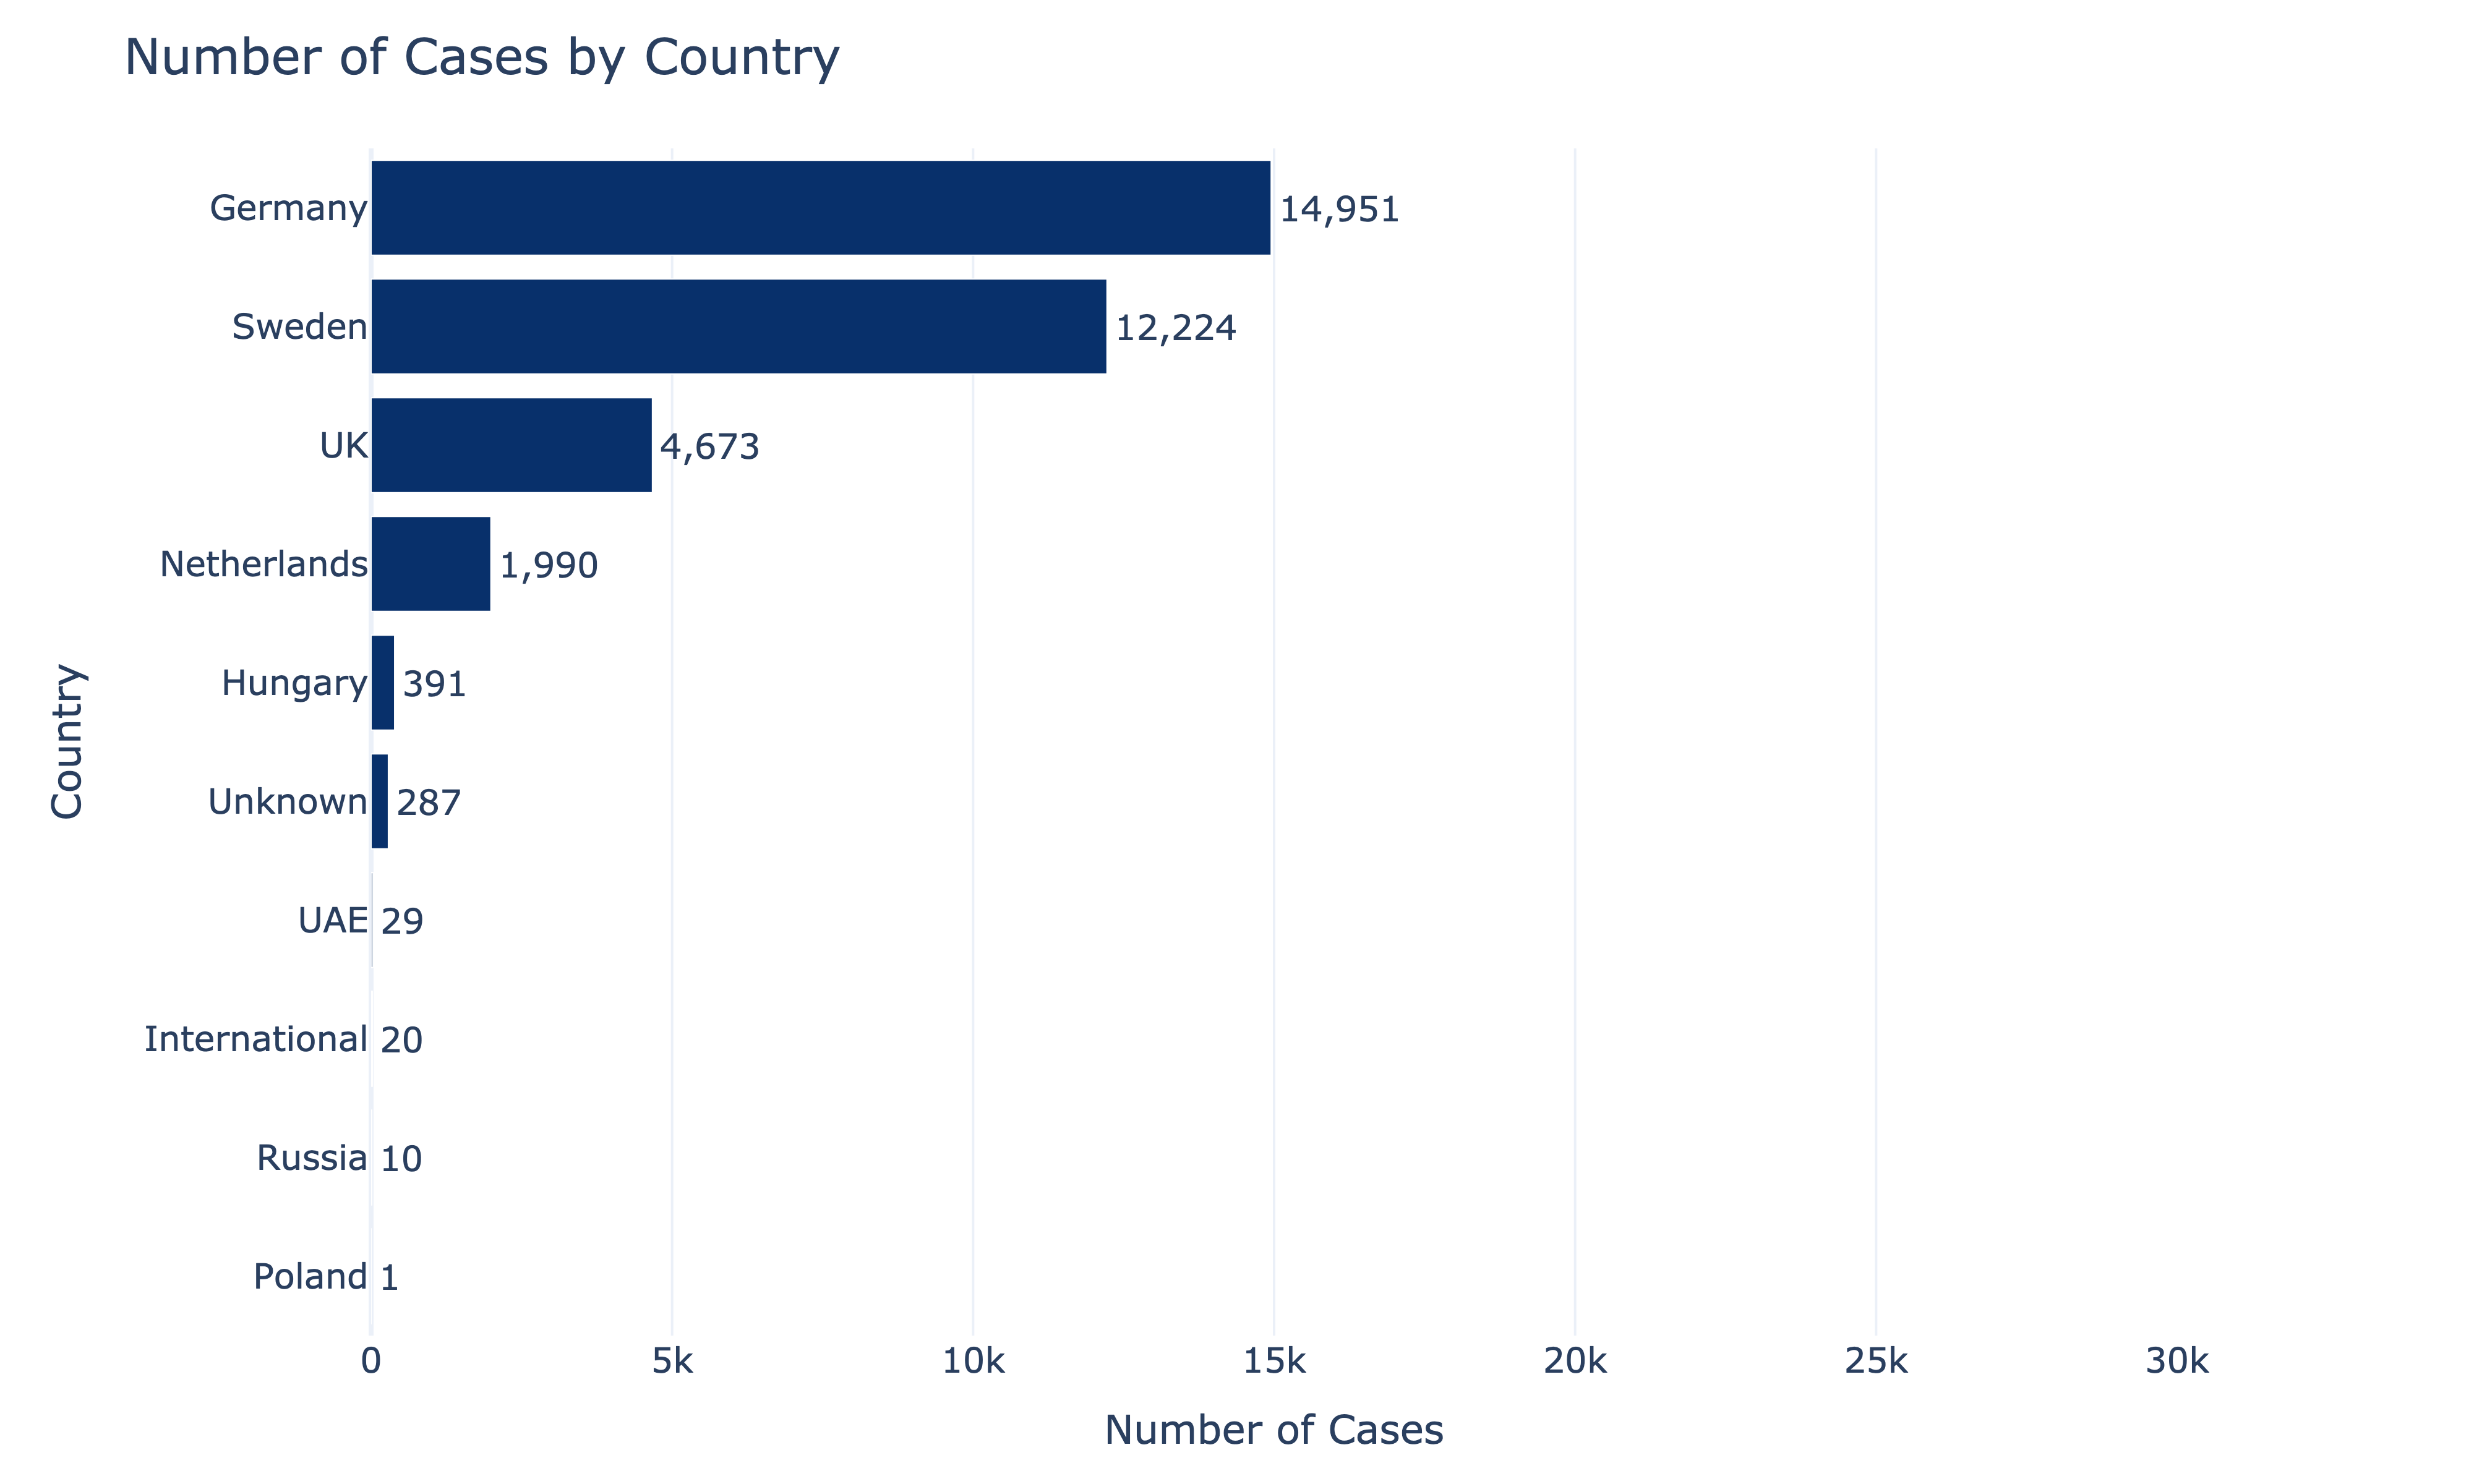
\includegraphics[width=\textwidth]{Results/_iteration_0/Number of Cases by Country.png}
        \caption{Distribution of cleaned incident records by country.}
        \label{fig:cases_by_country}
    \end{subfigure}
    \hfill
    \begin{subfigure}[t]{0.54\textwidth}
        \vspace{0pt}
        \centering
        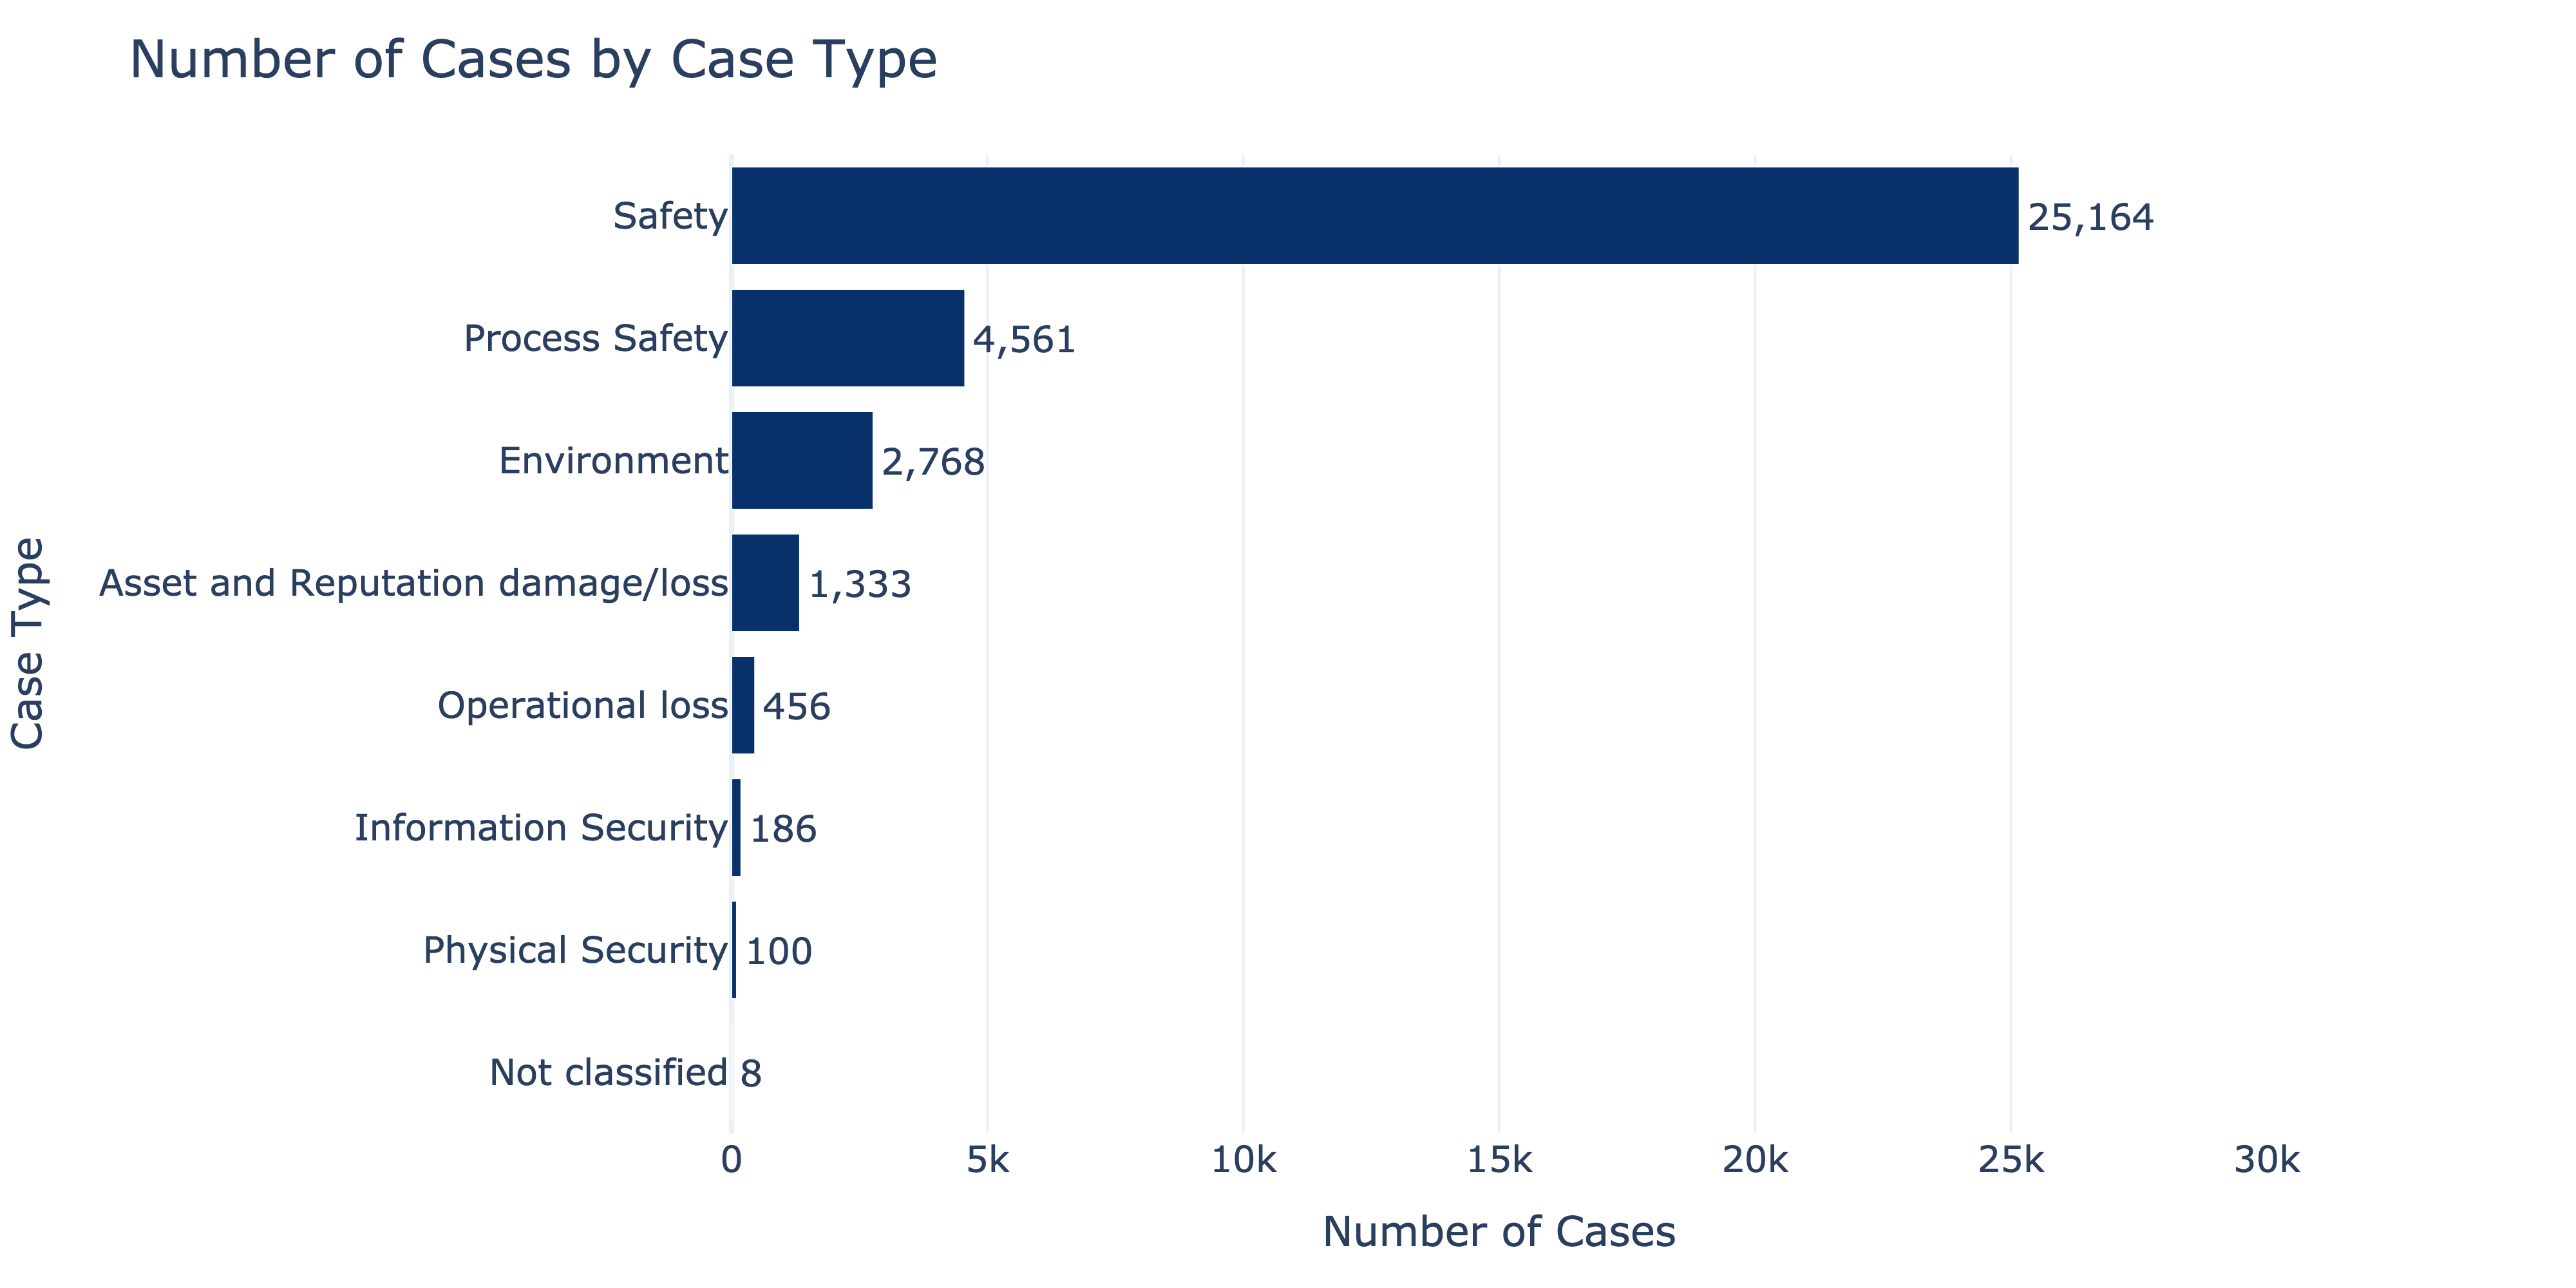
\includegraphics[width=\textwidth]{Results/_iteration_0/Number of Cases by Case Type.png}
        \caption{Distribution of cleaned incident records by case type.}
        \label{fig:cases_by_case_type}
    \end{subfigure}

    \caption{Country-level and case-type distributions of the cleaned Uniper HSSE master dataset.}
    \label{fig:dataset_distributions}
\end{figure}

Figure~\ref{fig:cases_by_country} shows that Germany contributes 14,951 records and Sweden 12,224 records, making these two countries the dominant sources of incident reports in the cleaned master dataset. The UK contributes 4,673 records and the Netherlands 1,990 records, while all remaining country groups contribute comparatively few cases. This imbalance has methodological consequences for multilingual modelling, since the effective representation of languages and reporting styles is not uniform across the corpus.

Figure~\ref{fig:cases_by_case_type} shows that the case-type distribution is also strongly imbalanced. The largest class is \textit{Safety} with 25,164 records, followed by \textit{Process Safety} with 4,561 and \textit{Environment} with 2,768. The remaining categories are substantially smaller: \textit{Asset and Reputation damage/loss} (1,333), \textit{Operational loss} (456), \textit{Information Security} (186), \textit{Physical Security} (100), and \textit{Not classified} (8). This imbalance provides an important methodological justification for later binary reformulation, class balancing, and macro-F1-based evaluation.

\subsection{Relationship to the Iteration~0 English Subsets}

The cleaned master dataset served as the source pool for the English-language subsets used in Iteration~0. From this master dataset, three alternative English subsets were created using different subset construction strategies: a manually curated English subset, a \texttt{langdetect}-based subset, and a \texttt{lingua}-based subset. These yielded 4,713, 6,002, and 6,205 records, respectively. The manually curated English subset was later selected as the official Iteration~0 baseline because it achieved the strongest macro-F1 score in the initial BERT+SVM experiment.

\subsection{External Datasets Explored but Not Included}

In addition to the internal Uniper HSSE reporting data, several external datasets were explored during the early scoping phase of the thesis. These included OSHA IMIS narratives, MSHA injury narratives, Dutch health complaint datasets, and UK Environment Agency CICS summaries. Although these datasets were initially considered as potential supplements for enlarging the corpus or enriching category diversity, they were ultimately not included in the final experimental dataset.

The main reason for exclusion was insufficient alignment with the structure and business context of the Uniper HSSE reporting environment. The external datasets differ substantially from the Uniper corpus in at least four ways. First, their label systems and incident taxonomies are defined for different regulatory or organisational settings, which makes direct category mapping unreliable. Second, the narrative style and reporting granularity differ from the internal Uniper HSSE reports, reducing comparability at the text level. Third, the domain emphasis of these external datasets is not fully consistent with the industrial Process Safety framing of this study; some are more strongly oriented toward occupational injury, public complaints, or environmental compliance narratives. Fourth, integrating them would have introduced substantial domain shift, which would have weakened the internal validity of the comparative experiments.

For these reasons, the final thesis experiments were restricted to the harmonised Uniper HSSE master dataset and the language-specific subsets derived from it. This ensured that the classification task remained closely aligned with the actual business case, the internal reporting taxonomy, and the multilingual incident-reporting environment relevant to the thesis objectives.

%------------------Table-------------------------
\begin{table}[h!]
\centering
\caption{Examples of raw incident reports illustrating data quality issues.}
\label{tab:rawdata}
\begin{footnotesize}
\begin{tabular}{p{1.3cm} p{8.2cm} p{6.5cm}}
\toprule
\textbf{Location} & \textbf{Title and Description} & \textbf{Potential Concerns} \\
\midrule
NL & \textbf{Title:} Overflow buffer B\newline \textbf{Description:} Buffer B is over gelopen door een bedieningsfout op buffer A. Tijdens het overzetten van de buffers omdat buffer B vol was is de retourwaterafsluiter van buffer A open gezet terwijl de aanvoerwaterafsluiter dicht stond. Dit heeft geresulteerd in het overlopen van buffer B met heet water (ca.~96$^\circ$C). Doordat dit een stoompluim op het dak van de buffer gaf, was de brandweer verwittigd. & Title is in English, but the description is in Dutch. \\
\addlinespace
NL & \textbf{Title:} Object falling from height -- GT3 enclosure\newline \textbf{Description:} While working with the chain hoist to remove parts of the turbine, the hoist's chain came into contact with an electrical distribution box. The distribution box was sealed with an iron cover tied down with strings. Due to the contact, the cover became loose and fell down where employees were working. The cover narrowly missed hitting a worker at ground level. & Report from NL but written in English. \\
\addlinespace
UK & \textbf{Title:} Environmental agency not correctly informed of GT12 fire at Killingholme power station\newline \textbf{Description:} Following an uncontrolled fire at the Killingholme power station, the Environment Agency was not informed. Site procedures were not clear about the requirement. & Grammatical errors in the description. \\
\addlinespace
NL & \textbf{Title:} Geen BMC meer op Roca\newline \textbf{Description:} Door storing geen BMC op Roca. & Description too short. Recommended description length is at least 50--100 words. \\
\addlinespace
NO & \textbf{Title:} Se över allmän belysning i DC.\newline \textbf{Description:} Se över allmän belysning i DC. & Description too short. Similar issues observed in reports from Sweden (due to data protection regulations). \\
\addlinespace
UK & \textbf{Title:} Steam Turbine Safety System Transmitter changed without Modification Process Followed\newline \textbf{Description:} One of the condenser level transmitters was replaced with a different make and model without following the proper modification process. This transmitter is part of the Steam Turbine SIL (Safety Integrity Level) rated protection functions. The modification process is intended to ensure any new transmitter meets the required reliability calculations from the Safety Manual and maintains the integrity of the protective function. There is a risk that the safety system’s integrity has been compromised without due diligence. & Context-specific abbreviations (e.g., ``SIL'' for Safety Integrity Level). \\
\addlinespace
NIL & \textbf{Title:} Safety Walk Betrieb\newline \textbf{Description:} 47319 An dem Kran in der benachbarten Halle der Wasseraufbereitung ist zu prüfen, ob die Bedieneinheit korrekt positioniert ist. & Location missing in dataset. \\
\bottomrule
\end{tabular}
\end{footnotesize}
\end{table}

\section{Data Preprocessing}

Before modelling, several preprocessing steps were applied to improve data quality and prepare the incident narratives for downstream machine learning experiments:

\begin{itemize}
    \item \textit{Data Anonymization:} Sensitive or business-critical information was removed or masked where necessary in order to protect confidentiality and reduce the risk of exposing internal operational details.
    
    \item \textit{Cleaning and Class Balancing:} Standard cleaning operations were applied, including the removal of invalid or incomplete entries, the treatment of missing values, and the normalisation of inconsistent textual content where appropriate. Because the classification task exhibits substantial class imbalance, class balancing strategies were later considered as part of the modelling pipeline.
    
    \item \textit{Tokenization and Lemmatization:} Text was segmented into tokens and standardised for NLP processing. Where relevant, words were reduced to their base forms to minimise variation caused by inflectional differences.
    
    \item \textit{Dataset Splitting:} The cleaned dataset was divided into training and test subsets in order to enable reproducible model training and evaluation.
\end{itemize}

\newpage

Table~\ref{tab:rawdata} presents representative examples of raw incident reports drawn from the industrial dataset. These examples highlight common data quality challenges encountered in real-world reporting, including multilingual descriptions, overly brief or incomplete narratives, grammatical errors, and the use of context-specific abbreviations. Together with the dataset-level imbalances shown in Figure~\ref{fig:dataset_distributions}, these issues illustrate the complexity of preparing incident reports for automated analysis and reinforce the need for robust preprocessing before reliable machine learning models can be trained.

\section{Model Development}

The model development strategy of this thesis follows an iterative experimental design. Rather than directly moving to advanced multilingual transformers or large language models, the research begins with a controlled baseline implementation and then progressively introduces additional complexity in later iterations. This approach makes it possible to identify the effect of individual methodological choices, isolate the contribution of specific components, and build a reproducible performance trajectory from a simple baseline to more advanced architectures.

The development process starts with a baseline binary classification setting in which incident reports are classified as either \textit{Process Safety} or \textit{Non-Process Safety}. The binary formulation was chosen intentionally, because Process Safety incidents represent the most business-critical class and therefore provide a focused first benchmark before moving to more complex multi-class and multilingual settings.

Iteration~0 serves as the experimental foundation of the thesis. It establishes the first end-to-end implementation pipeline, starting from cleaned and merged incident reports, continuing through English subset construction, exploratory data analysis, text embedding generation, and classifier training, and ending with an evaluation of three alternative English-language subset construction strategies. The strongest-performing strategy is then adopted as the official baseline for subsequent iterations.

\section{Iteration 0: Baseline Implementation}

\section{Iteration 0: Baseline Implementation}

\subsection{Overview and Motivation}
Iteration~0 establishes the foundational experimental pipeline for this thesis. Its primary objective is to create a reproducible and auditable baseline for Process Safety classification, and to rigorously evaluate how different English-language subset construction strategies affect downstream model performance. This baseline serves as the reference point for all subsequent methodological improvements and research targets.

\subsection{Experimental Scope and Subset Construction}
Three alternative English subset construction strategies were implemented and compared under an otherwise fixed modelling pipeline:
\begin{enumerate}
    \item \textbf{Manual English subset}: Formed by combining country-level files considered relevant for an English-language baseline (UK, UAE, Russia, Poland).
    \item \textbf{\texttt{langdetect}-based English subset}: Constructed automatically using probabilistic language detection (restricted to English, German, Swedish, Dutch, Hungarian).
    \item \textbf{\texttt{lingua}-based English subset}: Constructed automatically using a high-speed language detector over the same target language set.
\end{enumerate}

All three subsets were processed identically after construction. This allowed the baseline experiment to isolate the impact of English subset construction while keeping feature extraction and classification fixed.

\subsection{Integration with the Master Dataset}

Iteration~0 operates on the cleaned master dataset (34,576 records after deduplication and removal of missing values). The three English subsets were derived as follows:
\begin{itemize}
    \item \textbf{Manual}: 4,713 records (UK, UAE, Russia, Poland)
    \item \textbf{langdetect}: 6,014 records (automatic detection)
    \item \textbf{lingua}: 6,205 records (automatic detection)
\end{itemize}

\subsection{Exploratory Text Analysis}

Before modelling, an exploratory analysis of text length and lexical sparsity was performed in order to understand the quality of the available report narratives and the potential limitations for transformer-based embedding generation.

\subsubsection{Character Count Analysis}

For the full cleaned master dataset, the character-length statistics were:

\begin{itemize}
    \item \textbf{Title length:} minimum 3, maximum 662, mean 54.7086, median 46
    \item \textbf{Description length:} minimum 1, maximum 6,583, mean 140.0750, median 82
    \item \textbf{Combined text length:} minimum 6, maximum 6,708, mean 194.7836, median 140
\end{itemize}

These values show that incident titles are usually short, while descriptions vary substantially, with a long right tail of very detailed reports.

\subsubsection{Word Count Analysis}

The word-count statistics were:

\begin{itemize}
    \item \textbf{Title word count:} minimum 1, maximum 92, mean 7.9015, median 6
    \item \textbf{Description word count:} minimum 1, maximum 953, mean 21.2266, median 12
    \item \textbf{Combined word count:} minimum 2, maximum 969, mean 29.1281, median 20
\end{itemize}

These results indicate that a large proportion of reports are relatively short, which is relevant for embedding quality and later classification performance.

\subsubsection{Low Word Count Analysis}

A dedicated low-word-count analysis was performed to estimate the proportion of narratives with very limited semantic content.

For word count thresholds of 3, 5, and 10 words, the following proportions were observed:

\begin{table}[h!]
\centering
\caption{Low word count analysis for the cleaned master dataset.}
\label{tab:iter0_low_word_count}
\begin{tabular}{lrrr}
\toprule
\textbf{Threshold} & \textbf{Title} & \textbf{Description} & \textbf{Combined Text} \\
\midrule
$\leq 3$ words  & 6,374 (18.4348\%) & 3,263 (9.4372\%) & 267 (0.7722\%) \\
$\leq 5$ words  & 13,952 (40.3517\%) & 7,189 (20.7919\%) & 1,230 (3.5574\%) \\
$\leq 10$ words & 26,613 (76.9696\%) & 15,432 (44.6321\%) & 7,288 (21.0782\%) \\
\bottomrule
\end{tabular}
\end{table}

The very high proportion of short titles and relatively short descriptions highlights an important limitation of the raw data: some reports provide only weak semantic signal for contextual embedding models. This observation is relevant for interpreting baseline performance and motivates later experiments with alternative subset construction strategies and more robust multilingual representations.

\begin{figure}[htbp]
    \centering
    \begin{subfigure}[b]{0.95\textwidth}
        \centering
        \includegraphics[width=\textwidth]{Images/iteration_0_figures/word_count_distribution.png}
        \caption{Histogram-based word count distribution for titles and descriptions.}
        \label{fig:iter0_word_count_hist}
    \end{subfigure}

    \vspace{1em}

    \begin{subfigure}[b]{0.95\textwidth}
        \centering
        \includegraphics[width=\textwidth]{Images/iteration_0_figures/word_count_distribution_log_scale.png}
        \caption{Line graph of title and description word count frequencies on a logarithmic scale.}
        \label{fig:iter0_word_count_log}
    \end{subfigure}

    \caption{Exploratory word count analysis for the cleaned master dataset used in Iteration~0.}
    \label{fig:iter0_word_count_analysis}
\end{figure}

Figures~\ref{fig:iter0_word_count_hist} and \ref{fig:iter0_word_count_log} further illustrate the strong right-skew in the text-length distribution. Most titles are very short, while description lengths vary widely and include a long tail of highly detailed reports.

\subsection{Binary Classification Formulation}

After constructing the three English subsets, each record was reformulated as a binary classification instance. Let $y_i$ denote the target label of report $i$. The label was defined as:

\begin{equation}
y_i =
\begin{cases}
1, & \text{if } \texttt{CASE\_TYPE}_i = \text{Process Safety},\\[0.5em]
0, & \text{otherwise}.
\end{cases}
\end{equation}

This binary formulation collapses all non-Process-Safety categories into a single negative class and yields the first operational baseline for the business problem.

The class distributions in the three English subsets were:

\begin{itemize}
    \item \textbf{manual:} 1,409 Process Safety and 3,304 Non-Process Safety records
    \item \textbf{langdetect:} 1,526 Process Safety and 4,488 Non-Process Safety records
    \item \textbf{lingua:} 1,522 Process Safety and 4,683 Non-Process Safety records
\end{itemize}

The combined text feature for each record was created as:

\begin{equation}
\texttt{text\_features}_i = \texttt{TITLE}_i \oplus \text{``.''} \oplus \texttt{CASE\_DESCRIPTION}_i,
\end{equation}

where $\oplus$ denotes string concatenation. This ensures that both the concise title and the richer narrative description contribute to the document representation.

\subsection{BERT Embedding Generation}

For all three English subsets, contextual document representations were generated using the pre-trained \texttt{bert-base-uncased} transformer model. The tokenizer and model were loaded from Hugging Face Transformers, and the model was used in evaluation mode.

The implementation used:
\begin{itemize}
    \item \textbf{model:} \texttt{bert-base-uncased}
    \item \textbf{pooling strategy:} \texttt{[CLS]} token embedding from the final hidden layer
    \item \textbf{embedding dimension:} 768
    \item \textbf{batch size:} 8
    \item \textbf{maximum sequence length:} 512 tokens
    \item \textbf{device:} CPU in the recorded notebook run
\end{itemize}

Formally, the document embedding was defined as:

\begin{equation}
\mathbf{h}_{\text{[CLS]}} = \text{BERT}\big([\texttt{[CLS]}] \oplus \text{tokens} \oplus [\texttt{[SEP]}]\big)[0] \in \mathbb{R}^{768}.
\end{equation}

The generated embedding matrices had the following dimensions:

\begin{itemize}
    \item \textbf{manual:} $(4713, 768)$
    \item \textbf{langdetect:} $(6014, 768)$
    \item \textbf{lingua:} $(6205, 768)$
\end{itemize}

Embeddings and labels were saved as \texttt{.npy} files for reproducibility and reuse in later experiments.

\subsection{Classifier Training and Evaluation Pipeline}


For each English subset, the following pipeline was applied:
\begin{enumerate}
    \item 80/20 stratified train--test split
    \item Standardisation of embedding features using \texttt{StandardScaler}
    \item Training an SVM classifier (RBF kernel, \texttt{class\_weight='balanced'})
    \item Evaluation using accuracy, macro-F1, weighted-F1, classification reports, and confusion matrices
\end{enumerate}

The train--test split counts were:

\begin{table}[h!]
\centering
\caption{Train--test split statistics for the three Iteration~0 English subsets.}
\label{tab:iter0_train_test_split}
\begin{tabular}{lrrrr}
\toprule
\textbf{Subset} & \textbf{Train} & \textbf{Test} & \textbf{Train PS / Non-PS} & \textbf{Test PS / Non-PS} \\
\midrule
manual     & 3,770 &   943 & 1,127 / 2,643 & 282 / 661 \\
langdetect & 4,811 & 1,203 & 1,221 / 3,590 & 305 / 898 \\
lingua     & 4,964 & 1,241 & 1,218 / 3,746 & 304 / 937 \\
\bottomrule
\end{tabular}
\end{table}

\subsubsection{Actual Implemented Classifier}


\textbf{Pipeline summary:} \textit{BERT-base-uncased [CLS] embeddings $\rightarrow$ StandardScaler $\rightarrow$ RBF SVM classifier}

\subsection{Iteration~0 Results}

Table~\ref{tab:iter0_comparison_summary} summarises the final performance of the three English subset construction strategies under the common BERT+SVM pipeline.

\begin{table}[h!]
\centering
\caption{Comparison of the three English subset construction strategies in Iteration~0.}
\label{tab:iter0_comparison_summary}
\begin{tabular}{lrrrrrr}
\toprule
\textbf{Subset} & \textbf{Total} & \textbf{Accuracy} & \textbf{Macro-F1} & \textbf{Weighted-F1} & \textbf{Best?} \\
\midrule
manual     & 4,713 & 0.8112 & 0.7825 & 0.8143 &  \\
langdetect & 6,014 & \textbf{0.8379} & \textbf{0.7914} & \textbf{0.8400} & $\checkmark$ \\
lingua     & 6,205 & 0.8251 & 0.7758 & 0.8295 &  \\
\bottomrule
\end{tabular}
\end{table}

The results show that the \texttt{langdetect}-based English subset is the strongest-performing baseline according to both accuracy and macro-F1. The \texttt{manual} subset performs second best, while the \texttt{lingua} subset, despite being the largest, performs slightly worse on the main evaluation metric.

\subsubsection{Detailed Classification Reports}

\begin{table}[h!]
\centering
\caption{Per-class performance across the three English subset construction strategies.}
\label{tab:iter0_per_class_metrics}
\begin{tabular}{llcccc}
\toprule
\textbf{Subset} & \textbf{Class} & \textbf{Precision} & \textbf{Recall} & \textbf{F1-score} & \textbf{Support} \\
\midrule
\multirow{2}{*}{manual}
    & Non-Process Safety & 0.8864 & 0.8381 & 0.8616 & 661 \\
    & Process Safety     & 0.6635 & 0.7482 & 0.7033 & 282 \\
\midrule
\multirow{2}{*}{langdetect}
    & Non-Process Safety & 0.9026 & 0.8775 & 0.8899 & 898 \\
    & Process Safety     & 0.6667 & 0.7213 & 0.6929 & 305 \\
\midrule
\multirow{2}{*}{lingua}
    & Non-Process Safety & 0.9063 & 0.8570 & 0.8810 & 937 \\
    & Process Safety     & 0.6225 & 0.7270 & 0.6707 & 304 \\
\bottomrule
\end{tabular}
\end{table}

These results indicate that the best subset is not determined solely by minority-class recall. The manual subset achieves the strongest Process Safety F1-score (0.7033), but the \texttt{langdetect} subset achieves substantially stronger overall balance across both classes, which leads to the highest macro-F1 (0.7914). This is why \texttt{langdetect} becomes the preferred baseline when the notebook output is treated as final.

\subsubsection{Confusion Matrix Analysis}

The confusion matrices for the three subset construction strategies are shown in Figure~\ref{fig:iter0_confusion_matrices}. They provide a direct view of the trade-off between false positives and false negatives across the three English baselines.

\begin{figure}[htbp]
    \centering
    \begin{subfigure}[b]{0.95\textwidth}
        \centering
        
\includegraphics[width=\textwidth]{Images/iteration_0_figures/confusion_matrix_manual.png}
        \caption{Manual English subset: TN=554, FP=107, FN=71, TP=211.}
        \label{fig:iter0_cm_manual}
    \end{subfigure}

    \vspace{1em}

    \begin{subfigure}[b]{0.95\textwidth}
        \centering
        
\includegraphics[width=\textwidth]{Images/iteration_0_figures/confusion_matrix_langdetect.png}
        \caption{Langdetect English subset. Replace this figure with the regenerated version matching the latest notebook output (TN=788, FP=110, FN=85, TP=220).}
        \label{fig:iter0_cm_langdetect}
    \end{subfigure}

    \vspace{1em}

    \begin{subfigure}[b]{0.95\textwidth}
        \centering
        
\includegraphics[width=\textwidth]{Images/iteration_0_figures/confusion_matrix_lingua.png}
        \caption{Lingua English subset: TN=803, FP=134, FN=83, TP=221.}
        \label{fig:iter0_cm_lingua}
    \end{subfigure}

    \caption{Confusion matrices for the three English subset construction strategies in Iteration~0.}
    \label{fig:iter0_confusion_matrices}
\end{figure}

For the \texttt{manual} subset, the classifier correctly identifies 554 Non-Process Safety and 211 Process Safety reports, while producing 107 false positives and 71 false negatives.

For the \texttt{langdetect} subset, the latest notebook output reports 788 true negatives, 110 false positives, 85 false negatives, and 220 true positives.

For the \texttt{lingua} subset, the classifier correctly identifies 803 Non-Process Safety and 221 Process Safety reports, while producing 134 false positives and 83 false negatives.

\subsection{Selection of the Official Iteration~0 Baseline}


\textbf{Official Iteration~0 Baseline:}
The \texttt{langdetect}-based English subset is the official baseline, achieving the highest accuracy (0.8379), macro-F1 (0.7914), and weighted-F1 (0.8400) in the latest notebook implementation. The pipeline is:
\begin{quote}
\textit{English subset constructed using \texttt{langdetect}, encoded with BERT-base-uncased [CLS] embeddings, scaled with StandardScaler, and classified using an RBF-kernel SVM.}
\end{quote}

\subsection{Gap to Research Target}


\textbf{Gap to Research Target:}
The macro-F1 of the official Iteration~0 baseline (0.7914) is 5.86 percentage points below the RQ1 target of 0.85:
\begin{equation}
0.85 - 0.7914 = 0.0586
\end{equation}

\begin{table}[h!]
\centering
\caption{Gap between the Iteration~0 subset strategies and the RQ1 target.}
\label{tab:iter0_gap_analysis}
\begin{tabular}{lccc}
\toprule
\textbf{Subset} & \textbf{Macro-F1} & \textbf{RQ1 Target} & \textbf{Gap} \\
\midrule
manual     & 0.7825 & 0.85 & 0.0675 \\
langdetect & 0.7914 & 0.85 & 0.0586 \\
lingua     & 0.7758 & 0.85 & 0.0742 \\
\bottomrule
\end{tabular}
\end{table}

\subsection{Summary of Iteration~0}

\subsection{Summary and Implications}
Iteration~0 establishes a robust, reproducible baseline for Process Safety classification. Key findings:
\begin{itemize}
    \item The method of English subset construction has a material impact on classification performance.
    \item Short and low-information narratives are a significant data-quality constraint for embedding-based models.
    \item The pipeline of BERT-base-uncased [CLS] embeddings, feature scaling, and RBF SVM yields a strong, transparent baseline.
    \item The langdetect-based English subset is the official baseline, with macro-F1 = 0.7914.
    \item The gap to the research target (macro-F1 $\geq$ 0.85) is 5.86 percentage points, motivating further methodological improvements in subsequent iterations.
\end{itemize}

This baseline provides a clear, auditable reference for all later experiments, which will build upon and extend this methodology toward stronger transformer architectures, multilingual modelling, class balancing, ensemble learning, and LLM-based approaches.

\subsection{Iteration 1: BERT-base-cased Baseline Implementation}

\subsubsection{Objective}
Establish a comprehensive baseline for process safety incident classification using BERT-base-cased embeddings across multiple geographic and linguistic datasets.

\subsubsection{Implementation Steps}

\paragraph{1. Data Consolidation and Preparation}
Three raw datasets were consolidated and cleaned:
\begin{itemize}
    \item \texttt{RW\_ACTUALS\_PS}: 14,672 records
    \item \texttt{RW\_ACTUALS\_ALL}: 28,193 records  
    \item \texttt{RW\_ACTUALS\_NH\_OBS}: 900,482 records
\end{itemize}

After removing duplicates, null values, and blank key fields (\texttt{CASENO}, \texttt{CASE\_DESCRIPTION}, \texttt{TITLE}), a master dataset of 54,750 valid incident records was created. The dataset was then stratified by country:
\begin{itemize}
    \item UK, Germany, Sweden, Netherlands, UAE, International (individual datasets)
    \item English (combined UK, UAE & International: 4,483 records)
    \item Master (all countries: 54,750 records)
\end{itemize}

\paragraph{2. Feature Engineering}
\begin{itemize}
    \item \textbf{Binary labels:} Process Safety (1) vs Non-Process Safety (0)
    \item \textbf{Text features:} Concatenation of incident fields
    \begin{equation}
    \text{text\_features} = \text{TITLE} \oplus \text{``.''}  \oplus \text{CASE\_DESCRIPTION}
    \end{equation}
\end{itemize}

\paragraph{3. Embedding Generation}
\begin{itemize}
    \item \textbf{Model:} BERT-base-cased pre-trained transformer
    \item \textbf{Embedding dimension:} 768-dimensional vectors
    \item \textbf{Method:} [CLS] token representation from final hidden layer
    \item \textbf{Batch processing:} batch\_size = 8 with progress tracking
    \item \textbf{Storage:} Serialized as pickle files with metadata
\end{itemize}

\paragraph{4. Model Training}
\begin{itemize}
    \item \textbf{Classifier:} Linear Support Vector Machine (SVM)
    \item \textbf{Class balancing:} \texttt{class\_weight='balanced'} to handle imbalance
    \item \textbf{Data split:} 80/20 train-test split (stratified, random\_state=42)
    \item \textbf{Training scope:} Independent model for each dataset
\end{itemize}

\paragraph{5. Evaluation Metrics}
For each dataset, the following metrics were computed:
\begin{itemize}
    \item Confusion matrix: True Negatives (TN), False Positives (FP), False Negatives (FN), True Positives (TP)
    \item Per-class metrics: Precision, Recall, F1-score for both classes
    \item Macro-averaged metrics: Precision, Recall, F1-score (primary metric)
    \item Error rates: False Positive Rate (FPR), False Negative Rate (FNR)
    \item Overall accuracy
\end{itemize}

\subsubsection{Results and Outputs}
\begin{itemize}
    \item \textbf{Embeddings:} Saved in \texttt{/Datasets/Embeddings/\_iteration\_1/bert-base-cased/}
    \item \textbf{Naming convention:} \texttt{\{dataset\}\_bert-base-cased\_embeddings.pkl}
    \item \textbf{Visualizations:} Confusion matrix heatmaps (300 DPI PNG files)
    \item \textbf{Summary:} CSV file with all metrics across datasets
    \item \textbf{Documentation:} Markdown tables for LaTeX integration
\end{itemize}

\subsubsection{Key Outcomes}
\begin{itemize}
    \item Successfully evaluated 6 datasets with macro F1-scores ranging from 0.86 to 0.89
    \item All evaluated datasets exceeded the target threshold of 0.81
    \item Best performance: UK dataset (Macro F1 = 0.8872)
    \item Multilingual capability demonstrated with non-English datasets (German, Swedish, Dutch)
    \item False Negative Rates ranged from 15.1\% to 21.4\%, highlighting areas for improvement
    \item Established reproducible pipeline with fixed random seeds and comprehensive metadata tracking
\end{itemize}

\subsection{Iteration 2: Multi-Model Comparative Evaluation}

\subsubsection{Objective}
Conduct a comprehensive comparative analysis of multiple pre-trained transformer models across diverse datasets to identify the optimal architecture for process safety incident classification.

\subsubsection{Implementation Steps}

\paragraph{1. Model Selection and Configuration}
Ten state-of-the-art transformer models were selected for evaluation:

\textbf{BERT Family:}
\begin{itemize}
    \item \texttt{bert-base-cased}: 110M parameters, 768-dimensional embeddings
    \item \texttt{bert-large-cased}: 340M parameters, 1024-dimensional embeddings
\end{itemize}

\textbf{RoBERTa Family:}
\begin{itemize}
    \item \texttt{roberta-base}: 125M parameters, robustly optimized BERT approach
    \item \texttt{roberta-large}: 355M parameters, enhanced pre-training
\end{itemize}

\textbf{Specialized Architectures:}
\begin{itemize}
    \item \texttt{distilbert-base-cased}: 66M parameters, distilled efficient variant
    \item \texttt{xlnet-base-cased}: 110M parameters, permutation language modeling
    \item \texttt{modernbert-base}: 139M parameters, modern architectural improvements
    \item \texttt{modernbert-large}: 395M parameters, scaled version
    \item \texttt{deberta-v3-base}: 184M parameters, disentangled attention mechanism
    \item \texttt{deberta-v3-large}: 435M parameters, enhanced disentangled attention
\end{itemize}

\paragraph{2. Dataset Selection}
Six country-specific datasets were processed (four datasets excluded due to insufficient sample sizes):

\textbf{Included Datasets:}
\begin{itemize}
    \item UK, Germany, Sweden, Netherlands, Master (combined), English (UK,  UAE \& International)
\end{itemize}

\textbf{Excluded Datasets:}
\begin{itemize}
    \item Hungary, International, Russia, UAE (insufficient sample size for stratified splitting)
\end{itemize}

Total model-dataset combinations: $6 \times 10 = 60$ experiments

\paragraph{3. Pipeline Architecture with Checkpointing}
A robust two-phase pipeline was implemented with comprehensive error handling and progress tracking:

\textbf{Phase 1: Embedding Generation}
\begin{itemize}
    \item Batch processing with \texttt{batch\_size=4} for memory efficiency
    \item GPU acceleration when available with automatic fallback to CPU
    \item Periodic memory clearing: \texttt{torch.cuda.empty\_cache()} after each batch
    \item Maximum sequence length: 512 tokens with truncation
    \item Checkpoint saved after each successful dataset-model combination
\end{itemize}

\textbf{Phase 2: SVM Training and Evaluation}
\begin{itemize}
    \item Classifier: \texttt{LinearSVC} for computational efficiency
    \item Subsampling: Large training sets (>60,000 samples) reduced via stratified resampling
    \item Training timeout: 300 seconds per model to prevent hanging
    \item Class balancing: \texttt{class\_weight='balanced'}
    \item Hyperparameters: \texttt{max\_iter=1000}, \texttt{dual=False}, \texttt{random\_state=42}
\end{itemize}

\paragraph{4. Checkpoint System Implementation}
A JSON-based checkpoint system enabled resumable execution:
\begin{itemize}
    \item Checkpoint file: \texttt{checkpoint.json} tracking completed (model, dataset) tuples
    \item Automatic skip of processed combinations on restart
    \item Utility functions: \texttt{view\_progress()}, \texttt{reset\_checkpoint()}, \texttt{complete\_rerun()}
    \item Progress persistence across kernel restarts and failures
\end{itemize}

\paragraph{5. Memory Management Strategy}
Aggressive memory management prevented out-of-memory errors:
\begin{itemize}
    \item Batch-level GPU memory clearing
    \item Periodic garbage collection every 50 batches
    \item Model unloading between experiments
    \item Explicit deletion of large variables: \texttt{del} followed by \texttt{gc.collect()}
    \item Dataset subsampling for SVM training when necessary
\end{itemize}

\paragraph{6. Comprehensive Evaluation Metrics}
For each model-dataset combination, the following metrics were computed:

\textbf{Overall Metrics:}
\begin{itemize}
    \item Accuracy: $\frac{TP + TN}{TP + TN + FP + FN}$
    \item Macro-averaged F1-score: $\frac{F1_{\text{PS}} + F1_{\text{NPS}}}{2}$
    \item Weighted F1-score: $\frac{\sum_{c} F1_c \times \text{support}_c}{\sum_{c} \text{support}_c}$
\end{itemize}

\textbf{Per-Class Metrics (Process Safety and Non-Process Safety):}
\begin{itemize}
    \item Precision: $\frac{TP}{TP + FP}$
    \item Recall: $\frac{TP}{TP + FN}$
    \item F1-score: $\frac{2 \times \text{Precision} \times \text{Recall}}{\text{Precision} + \text{Recall}}$
    \item Support: Number of true instances per class
\end{itemize}

\textbf{Additional Tracking:}
\begin{itemize}
    \item Training time (seconds)
    \item Subsampling flag (indicating whether training set was reduced)
    \item Confusion matrix elements: TN, FP, FN, TP
\end{itemize}

\paragraph{7. Visualization and Reporting}
\begin{itemize}
    \item Confusion matrix heatmaps for each combination (300 DPI, PNG format)
    \item Naming convention: \texttt{cm\_\{dataset\}\_\{model\}.png}
    \item Comprehensive CSV export with all metrics
    \item Formatted classification reports mimicking \texttt{sklearn} style
    \item Aggregate statistics by model and by dataset
\end{itemize}

\subsubsection{Results and Outputs}

\paragraph{Storage Structure}
\begin{itemize}
    \item \textbf{Embeddings:} \texttt{/Datasets/Embeddings/\_iteration\_2/\{model\_name\}/}
    \item \textbf{Results:} \texttt{/Results/\_iteration\_2/}
    \item \textbf{Checkpoint:} \texttt{/\_iteration\_2/checkpoint.json}
    \item \textbf{Summary:} \texttt{all\_models\_svm\_detailed\_results.csv}
\end{itemize}

\paragraph{Aggregate Analysis}
Multiple aggregate views were generated:

\textbf{By Model Performance:}
\begin{itemize}
    \item Mean and standard deviation of accuracy, F1 scores across all datasets
    \item Identification of consistently high-performing architectures
    \item Stability analysis via standard deviation metrics
\end{itemize}

\textbf{By Dataset Characteristics:}
\begin{itemize}
    \item Mean and standard deviation of metrics across all models
    \item Dataset difficulty assessment
    \item Language-specific performance patterns (English vs. non-English)
\end{itemize}

\textbf{Best Performing Combinations:}
\begin{itemize}
    \item Top model by overall accuracy
    \item Best model for Process Safety class F1-score (critical for safety applications)
    \item Most efficient model (considering training time vs. performance trade-off)
\end{itemize}

\subsubsection{Key Innovations}

\paragraph{1. Scalability}
The pipeline processed 60 model-dataset combinations with automatic recovery from failures, enabling large-scale comparative studies without manual intervention.

\paragraph{2. Reproducibility}
Fixed random seeds (\texttt{random\_state=42}), comprehensive metadata tracking, and version-controlled model names ensured full experimental reproducibility.

\paragraph{3. Efficiency}
\begin{itemize}
    \item Checkpoint system eliminated redundant computation
    \item Strategic subsampling balanced computational cost with statistical validity
    \item Batch processing and memory management enabled processing on resource-constrained hardware
\end{itemize}

\paragraph{4. Robustness}
\begin{itemize}
    \item Timeout protection prevented infinite loops
    \item Exception handling with detailed error logging
    \item Graceful degradation (skip failed combinations, continue pipeline)
\end{itemize}

\subsubsection{Limitations and Observations}

\begin{itemize}
    \item \textbf{Computational Cost:} Large models (\texttt{deberta-v3-large}, \texttt{modernbert-large}) required significant processing time (3+ hours per dataset)
    \item \textbf{Subsampling Trade-off:} Training set reduction for large datasets may have slightly reduced model performance
    \item \textbf{Model Failures:} Four models (\texttt{modernbert-base}, \texttt{modernbert-large}, \texttt{deberta-v3-base}, \texttt{deberta-v3-large}) encountered compatibility issues with certain datasets
    \item \textbf{Linear Classification:} Use of LinearSVC instead of kernel SVM may have limited decision boundary complexity
    \item \textbf{Language Mismatch:} English-trained models applied to German, Swedish, and Dutch datasets may not capture language-specific semantics optimally
\end{itemize}

These observations informed the design of Iteration 3, which explores domain-specific fine-tuning and multilingual transformer architectures to address the identified limitations.

\subsection{Iteration 3: Multilingual Transformer Evaluation}

\subsubsection{Objective}
Evaluate specialized multilingual transformer models to address the language mismatch limitation identified in Iteration 2, where English-trained models were applied to non-English datasets (German, Swedish, Dutch).

\subsubsection{Rationale}
Previous iterations demonstrated that monolingual English models (BERT-base-cased, RoBERTa) achieved strong performance on English datasets but exhibited suboptimal results on non-English data. Multilingual models, pre-trained on diverse language corpora, provide native cross-lingual capabilities that may better capture semantic relationships in multilingual safety incident reports.

\subsubsection{Implementation Steps}

\paragraph{1. Multilingual Model Selection}
Five state-of-the-art multilingual transformer models were selected based on their language coverage and architectural innovations:

\textbf{BERT Multilingual Variants:}
\begin{itemize}
    \item \texttt{bert-base-multilingual-uncased}: 110M parameters, trained on 104 languages, case-insensitive tokenization
    \item \texttt{bert-base-multilingual-cased}: 110M parameters, trained on 104 languages, preserves case information
\end{itemize}

\textbf{E5 Embedding Models (Multilingual):}
\begin{itemize}
    \item \texttt{intfloat/multilingual-e5-base}: Text embedding model optimized for semantic similarity across more than 100 languages
    \item \texttt{intfloat/multilingual-e5-large}: Scaled version with enhanced embedding quality (560M parameters)
    \item \texttt{intfloat/multilingual-e5-large-instruct}: Instruction-tuned variant for improved task-specific performance
\end{itemize}

The E5 (Embeddings from bidirectional Encoder representations) models represent a family of text embeddings optimized for semantic search and similarity tasks, with explicit multilingual training objectives.

\paragraph{2. Dataset Configuration}
Consistent with Iteration 2, six datasets were processed:

\textbf{Included Datasets:}
\begin{itemize}
    \item UK (English)
    \item Germany (German)
    \item Sweden (Swedish)
    \item Netherlands (Dutch)
    \item Master (all countries combined)
    \item English (UK, UAE \& International combined)
\end{itemize}

\textbf{Excluded Datasets:}
\begin{itemize}
    \item Hungary, International, Russia, UAE (insufficient samples for stratified splitting)
\end{itemize}

Total model-dataset combinations: $6 \times 5 = 30$ experiments

\paragraph{3. Pipeline Architecture}
The implementation followed a two-phase architecture identical to Iteration 2, with optimizations for multilingual tokenization:

\textbf{Phase 1: Embedding Generation}
\begin{itemize}
    \item Tokenizer initialization with \texttt{trust\_remote\_code=True} for model-specific implementations
    \item Automatic padding token configuration for models lacking default padding:
    \begin{equation}
    \text{tokenizer.pad\_token} = \text{tokenizer.eos\_token}
    \end{equation}
    \item Batch size: 8 (increased from Iteration 2's batch size of 4 due to smaller model sizes)
    \item Maximum sequence length: 512 tokens with truncation
    \item Device-aware processing: automatic GPU utilization when available
    \item Memory management: periodic cache clearing every 50 batches
\end{itemize}

\textbf{Phase 2: Classification and Evaluation}
\begin{itemize}
    \item Classifier: \texttt{LinearSVC} with \texttt{dual=False} optimization
    \item Training set subsampling: Maximum 60,000 samples via stratified resampling
    \item Class balancing: \texttt{class\_weight='balanced'}
    \item Hyperparameters: \texttt{max\_iter=1000}, \texttt{random\_state=42}
\end{itemize}

\paragraph{4. Feature Engineering}
Text features were constructed identically to previous iterations:
\begin{equation}
\text{text\_features} = \text{TITLE} \oplus \text{``.''}  \oplus \text{CASE\_DESCRIPTION}
\end{equation}

This concatenation strategy provides both concise summaries (TITLE) and detailed contextual information (CASE\_DESCRIPTION) to the multilingual encoders.

\paragraph{5. Checkpoint and Recovery System}
A robust checkpoint system enabled resumable execution:

\textbf{Checkpoint Functions:}
\begin{itemize}
    \item \texttt{save\_checkpoint(processed\_items)}: Serialize completed (model, dataset) combinations to JSON
    \item \texttt{load\_checkpoint()}: Restore progress from checkpoint file
    \item \texttt{view\_progress()}: Display processed combinations
    \item \texttt{reset\_checkpoint()}: Clear checkpoint for fresh restart
\end{itemize}

\textbf{Progress Tracking:}
\begin{itemize}
    \item Checkpoint saved after each successful embedding generation
    \item Automatic skip of already-processed combinations on restart
    \item Progress indicator: \texttt{processed/total} combinations
    \item Persistent storage: \texttt{/\_Iterations/\_iteration\_3/checkpoint.json}
\end{itemize}

\paragraph{6. Embedding Generation Function}
A unified embedding function handled both standard BERT and specialized E5 models:

\begin{lstlisting}[language=Python, caption=Unified Embedding Generation]
def get_bert_embeddings(texts, tokenizer, model, 
                        max_length=512, batch_size=8):
    """Generate embeddings (works for BERT and E5 models)"""
    embeddings = []
    device = 'cuda' if torch.cuda.is_available() else 'cpu'
    model = model.to(device)
    
    for batch_texts in batches(texts, batch_size):
        inputs = tokenizer(
            batch_texts,
            padding=True,
            truncation=True,
            max_length=max_length,
            return_tensors="pt"
        ).to(device)
        
        with torch.no_grad():
            outputs = model(**inputs)
            # Use [CLS] token representation
            if hasattr(outputs, 'last_hidden_state'):
                batch_embeddings = outputs.last_hidden_state[:, 0, :].cpu().numpy()
            else:
                # Fallback for different output structures
                batch_embeddings = outputs[0][:, 0, :].cpu().numpy()
            embeddings.extend(batch_embeddings)
        
        # Memory management
        if device == 'cuda':
            torch.cuda.empty_cache()
        if batch_idx % 50 == 0:
            gc.collect()
    
    return np.array(embeddings)
\end{lstlisting}

The function includes fallback logic for models with varying output structures, ensuring compatibility across the diverse E5 and BERT architectures.

\paragraph{7. Comprehensive Evaluation Metrics}
Identical to Iteration 2, the following metrics were computed:

\textbf{Overall Performance:}
\begin{itemize}
    \item Accuracy: $\frac{TP + TN}{TP + TN + FP + FN}$
    \item Weighted F1-score: $\sum_{c \in \{\text{PS, NPS}\}} F1_c \times \frac{\text{support}_c}{\text{total support}}$
    \item Macro F1-score: $\frac{F1_{\text{PS}} + F1_{\text{NPS}}}{2}$ (primary metric)
\end{itemize}

\textbf{Per-Class Metrics (both classes):}
\begin{itemize}
    \item Precision, Recall, F1-score, Support
\end{itemize}

\textbf{Training Metadata:}
\begin{itemize}
    \item Training time (seconds)
    \item Subsampling indicator
    \item Confusion matrix: TN, FP, FN, TP
\end{itemize}

\paragraph{8. Results Storage and Visualization}
\textbf{Storage Structure:}
\begin{itemize}
    \item \textbf{Embeddings:} \texttt{/Datasets/Embeddings/\_iteration\_3/\{model\_key\}/}
    \item \textbf{Results:} \texttt{/Results/\_iteration\_3/}
    \item \textbf{Summary:} \texttt{multi\_model\_svm\_results.csv}
    \item \textbf{Visualizations:} Confusion matrix heatmaps (300 DPI PNG)
\end{itemize}

\textbf{Naming Convention:}
\begin{itemize}
    \item Embeddings: \texttt{\{dataset\}\_\{model\_key\}\_embeddings.pkl}
    \item Confusion matrices: \texttt{cm\_\{dataset\}\_\{model\_key\}.png}
\end{itemize}

\subsubsection{Results Analysis Framework}

\paragraph{Multi-Dimensional Comparative Analysis}
Results were analyzed across three dimensions:

\textbf{1. Model Comparison:}
\begin{itemize}
    \item Aggregate statistics (mean, standard deviation) of accuracy, F1-scores, and per-class metrics across all datasets
    \item Identification of consistently high-performing architectures
    \item Stability analysis via cross-dataset standard deviation
\end{itemize}

\textbf{2. Dataset Comparison:}
\begin{itemize}
    \item Average performance across all models per dataset
    \item Language-specific performance patterns (English vs. German vs. Swedish vs. Dutch)
    \item Dataset difficulty ranking based on average F1-scores
\end{itemize}

\textbf{3. Best Performers:}
\begin{itemize}
    \item Highest accuracy combination
    \item Best Process Safety F1-score (critical for safety applications)
    \item Most efficient model (accuracy per training time)
\end{itemize}


%\paragraph{Classification Report Generation}
%For each model-dataset combination, sklearn-style classification reports were generated:

%\begin{table}[htbp]
%\centering
%\small
%\begin{tabular}{@{}lcccc@{}}
%\toprule
%\textbf{Class} & \textbf{Precision} & \textbf{Recall} & \textbf{F1-score} & \textbf{Support} \\
%\midrule
%Non-Process Safety   & 0.XX & 0.XX & 0.XX & XXXX \\
%Process Safety       & 0.XX & 0.XX & 0.XX & XXX \\
%\midrule
%accuracy             &      &      & 0.XX & XXXX \\
%macro avg            & 0.XX & 0.XX & 0.XX & XXXX \\
%weighted avg         & 0.XX & 0.XX & 0.XX & XXXX \\
%\bottomrule
%\end{tabular}
%\caption{Example classification report structure for Iteration 3 results}
%\end{table}

\subsubsection{Key Innovations}

\paragraph{1. Language-Aware Architecture}
Multilingual models eliminate the language mismatch problem, providing native support for German, Swedish, and Dutch incident reports without requiring translation or language-specific fine-tuning.

\paragraph{2. E5 Embedding Models}
Integration of E5 models introduces contrastive learning-based embeddings optimized for semantic similarity, potentially capturing incident similarity relationships more effectively than traditional masked language models.

\paragraph{3. Instruction Tuning}
The \texttt{multilingual-e5-large-instruct} model incorporates instruction-following capabilities, enabling task-specific optimization through natural language instructions (though not explicitly utilized in this iteration).

\paragraph{4. Unified Embedding Interface}
The generalized embedding function abstracts model-specific implementation details, enabling seamless integration of future transformer architectures with minimal code modification.

\paragraph{5. Enhanced Checkpoint Granularity}
Checkpoint system tracks individual (model, dataset) combinations rather than full model completion, minimizing wasted computation on partial failures.

\subsubsection{Expected Outcomes}

Based on multilingual model capabilities, the following outcomes are anticipated:

\begin{itemize}
    \item \textbf{Non-English Dataset Improvement:} Multilingual BERT variants should outperform monolingual BERT on German, Swedish, and Dutch datasets by 5-10 percentage points in macro F1-score
    \item \textbf{English Dataset Parity:} Performance on English datasets should match or slightly trail Iteration 2 monolingual models due to diluted language-specific knowledge
    \item \textbf{E5 Model Performance:} E5-large models should demonstrate superior semantic understanding, particularly for capturing incident similarity patterns
    \item \textbf{Cross-Lingual Transfer:} Master dataset (combining all languages) should benefit most from multilingual architectures, demonstrating effective cross-lingual knowledge transfer
\end{itemize}

\subsubsection{Limitations and Considerations}

\begin{itemize}
    \item \textbf{Computational Cost:} Multilingual models, despite similar parameter counts to monolingual BERT, may exhibit longer inference times due to larger vocabulary sizes (104 languages vs. English-only)
    \item \textbf{Language Distribution Bias:} Multilingual BERT was pre-trained on imbalanced language corpora, potentially favoring high-resource languages (English, German) over low-resource languages (Swedish, Dutch)
    \item \textbf{Domain Shift:} Pre-training corpora consist primarily of Wikipedia and web text, differing significantly from technical safety incident reports
    \item \textbf{Tokenization Challenges:} Multilingual tokenizers may fragment technical terminology (e.g., equipment names, chemical compounds) more aggressively than domain-specific tokenizers
    \item \textbf{E5 Model Constraints:} E5 models were optimized for semantic similarity tasks, not classification—requiring adaptation via SVM may not fully exploit their capabilities
\end{itemize}

\subsubsection{Comparison with Previous Iterations}

\begin{table}[htbp]
\centering
\small
\begin{tabular}{@{}llll@{}}
\toprule
\textbf{Aspect} & \textbf{Iteration 1} & \textbf{Iteration 2} & \textbf{Iteration 3} \\
\midrule
Models & 1 (BERT-base-cased) & 10 (diverse) & 5 (multilingual) \\
Datasets & 6 & 6 & 6 \\
Combinations & 6 & 60 & 30 \\
Language Support & English only & English only & 104 languages \\
Batch Size & 8 & 4 & 8 \\
Primary Focus & Baseline & Architecture comparison & Language coverage \\
Key Innovation & Stratification & Checkpointing & Multilingual embeddings \\
\bottomrule
\end{tabular}
\caption{Comparison of Iterations 1-3}
\label{tab:iteration_comparison}
\end{table}

These observations inform the design of Iteration 4, which explores domain-specific fine-tuning of the best-performing multilingual models on process safety incident data to further enhance classification accuracy and address the domain shift limitation.

\subsection{Iteration 4: Advanced Machine Learning Pipeline with Enhanced Techniques}

\subsubsection{Objective}
Implement a comprehensive machine learning pipeline incorporating advanced techniques to maximize classification performance through improved embedding strategies, class imbalance handling, multiple classifier architectures, hyperparameter optimization, and ensemble methods.

\subsubsection{Rationale}
Previous iterations identified several optimization opportunities: (1) [CLS] token embeddings may not fully capture document semantics, (2) severe class imbalance (Process Safety incidents constitute 10-20\% of datasets) degrades minority class recall, (3) LinearSVC may not represent the optimal classifier architecture, and (4) single-model predictions lack robustness. Iteration 4 addresses these limitations through a multi-faceted enhancement strategy.

\subsubsection{Implementation Steps}

\paragraph{1. Model Selection and Configuration}
Three high-performing multilingual models from Iteration 3 were selected:

\begin{itemize}
    \item \texttt{bert-base-multilingual-uncased}: 110M parameters, 104 languages
    \item \texttt{xlm-roberta-base}: 270M parameters, cross-lingual robustly optimized architecture for 100 languages
    \item \texttt{sentence-transformers/paraphrase-multilingual-mpnet-base-v2}: Sentence-BERT variant optimized for semantic similarity, 278M parameters
\end{itemize}

Total model-dataset combinations: $3 \times 6 = 18$ base experiments, expanded to $18 \times 5 = 90$ classifier combinations.

\paragraph{2. Enhanced Configuration Framework}
A comprehensive configuration dictionary controlled all pipeline parameters:

\begin{lstlisting}[language=Python, caption=Iteration 4 Configuration]
CONFIG = {
    'pooling_strategy': 'mean',        # 'cls', 'mean', or 'max'
    'use_smote': True,                 # Class balancing
    'smote_strategy': 0.7,             # Minority: 70% of majority
    'use_feature_scaling': True,       # StandardScaler normalization
    'hyperparameter_tuning': True,     # GridSearchCV optimization
    'use_ensemble': True,              # Voting classifier
    'classifiers': ['svm', 'xgboost', 'lightgbm', 
                    'random_forest', 'ensemble'],
    'cv_folds': 5,                     # Cross-validation folds
    'text_preprocessing': True         # Advanced cleaning
}
\end{lstlisting}

This modular design enables ablation studies to quantify the contribution of individual enhancements.

\paragraph{3. Advanced Text Preprocessing}
Enhanced preprocessing addresses domain-specific noise in incident reports:

\begin{lstlisting}[language=Python, caption=Advanced Text Preprocessing]
def advanced_text_preprocessing(text):
    """Enhanced text preprocessing for incident reports"""
    if pd.isna(text):
        return ""
    
    # Convert to lowercase for uniformity
    text = str(text).lower()
    
    # Remove URLs (common in incident reports)
    text = re.sub(r'http\S+|www\S+|https\S+', '', text, 
                  flags=re.MULTILINE)
    
    # Remove email addresses (PII protection)
    text = re.sub(r'\S+@\S+', '', text)
    
    # Remove special characters, preserve sentence structure
    text = re.sub(r'[^a-zA-Z0-9\s\.]', ' ', text)
    
    # Remove extra whitespace
    text = ' '.join(text.split())
    
    return text
\end{lstlisting}

Preprocessing steps:
\begin{enumerate}
    \item Lowercase normalization
    \item URL removal (common in copy-pasted reports)
    \item Email address removal (privacy preservation)
    \item Special character filtering (preserve periods for sentence boundaries)
    \item Whitespace normalization
\end{enumerate}

\paragraph{4. Enhanced Embedding Generation with Pooling Strategies}
Three pooling strategies were implemented to aggregate token-level representations:

\textbf{CLS Pooling (Baseline):}
\begin{equation}
\mathbf{h}_{\text{CLS}} = \text{LastHiddenState}[:, 0, :]
\end{equation}

Uses the [CLS] token representation, standard in BERT-style models.

\textbf{Mean Pooling (Primary):}
\begin{equation}
\mathbf{h}_{\text{mean}} = \frac{\sum_{i=1}^{n} m_i \cdot \mathbf{h}_i}{\sum_{i=1}^{n} m_i}
\end{equation}

where $m_i$ is the attention mask for token $i$, and $\mathbf{h}_i$ is the hidden state. Mean pooling averages all token representations weighted by attention mask, capturing document-level semantics more comprehensively than [CLS] alone.

\textbf{Max Pooling (Alternative):}
\begin{equation}
\mathbf{h}_{\text{max}} = \max_{i=1}^{n} \mathbf{h}_i
\end{equation}

Max pooling selects the maximum activation across all token dimensions, emphasizing salient features.

Implementation:

\begin{lstlisting}[language=Python, caption=Enhanced Embedding Generation]
def get_enhanced_embeddings(texts, tokenizer, model, 
                            pooling='mean', max_length=512, 
                            batch_size=8):
    """Generate embeddings with advanced pooling strategies"""
    embeddings = []
    device = 'cuda' if torch.cuda.is_available() else 'cpu'
    model = model.to(device)
    model.eval()
    
    for batch_texts in tqdm(batches(texts, batch_size)):
        inputs = tokenizer(
            batch_texts,
            padding=True,
            truncation=True,
            max_length=max_length,
            return_tensors="pt"
        ).to(device)
        
        with torch.no_grad():
            outputs = model(**inputs)
            
            if pooling == 'cls':
                batch_embeddings = outputs.last_hidden_state[:, 0, :]
                
            elif pooling == 'mean':
                # Attention-mask weighted mean pooling
                attention_mask = inputs['attention_mask']
                token_embeddings = outputs.last_hidden_state
                input_mask_expanded = attention_mask.unsqueeze(-1).expand(
                    token_embeddings.size()).float()
                sum_embeddings = torch.sum(
                    token_embeddings * input_mask_expanded, 1)
                sum_mask = torch.clamp(
                    input_mask_expanded.sum(1), min=1e-9)
                batch_embeddings = (sum_embeddings / sum_mask)
                
            elif pooling == 'max':
                batch_embeddings = torch.max(
                    outputs.last_hidden_state, dim=1)[0]
            
            embeddings.extend(batch_embeddings.cpu().numpy())
        
        # Memory management
        if device == 'cuda':
            torch.cuda.empty_cache()
        if batch_idx % 50 == 0:
            gc.collect()
    
    return np.array(embeddings)
\end{lstlisting}

\paragraph{5. SMOTE-Based Class Balancing}
Synthetic Minority Over-sampling Technique (SMOTE) addresses severe class imbalance:

\textbf{Problem Formulation:}
\begin{itemize}
    \item Majority class (Non-Process Safety): 80-90\% of samples
    \item Minority class (Process Safety): 10-20\% of samples
    \item Consequence: Classifier bias toward majority class, poor minority recall
\end{itemize}

\textbf{SMOTE Algorithm:}
\begin{enumerate}
    \item For each minority class sample $\mathbf{x}_i$, identify $k$ nearest neighbors
    \item Randomly select one neighbor $\mathbf{x}_{\text{nn}}$
    \item Generate synthetic sample:
    \begin{equation}
    \mathbf{x}_{\text{new}} = \mathbf{x}_i + \lambda \cdot (\mathbf{x}_{\text{nn}} - \mathbf{x}_i)
    \end{equation}
    where $\lambda \sim \text{Uniform}(0, 1)$
    \item Repeat until minority class reaches target proportion
\end{enumerate}

\textbf{Implementation Parameters:}
\begin{itemize}
    \item \texttt{sampling\_strategy=0.7}: Oversample minority to 70\% of majority class size
    \item \texttt{k\_neighbors=5}: Use 5 nearest neighbors (or fewer if minority class $< 6$ samples)
    \item \texttt{random\_state=42}: Reproducibility
\end{itemize}

\begin{lstlisting}[language=Python, caption=SMOTE Application]
if CONFIG['use_smote'] and IMBLEARN_AVAILABLE:
    smote = SMOTE(
        sampling_strategy=CONFIG['smote_strategy'],
        random_state=42,
        k_neighbors=min(5, sum(y_train == 1) - 1)
    )
    X_train_balanced, y_train_balanced = smote.fit_resample(
        X_train, y_train)
    
    print(f"Original class distribution: {np.bincount(y_train)}")
    print(f"Balanced class distribution: {np.bincount(y_train_balanced)}")
\end{lstlisting}

\paragraph{6. Feature Scaling}
StandardScaler normalization ensures features have zero mean and unit variance:

\begin{equation}
\mathbf{x}_{\text{scaled}} = \frac{\mathbf{x} - \mu}{\sigma}
\end{equation}

where $\mu$ is the feature mean and $\sigma$ is the standard deviation computed on training data. This is critical for SVM and distance-based classifiers.

\begin{lstlisting}[language=Python, caption=Feature Scaling]
if CONFIG['use_feature_scaling']:
    scaler = StandardScaler()
    X_train_scaled = scaler.fit_transform(X_train_subset)
    X_test_scaled = scaler.transform(X_test)
\end{lstlisting}

\paragraph{7. Multiple Classifier Architectures}
Five classifier types were trained on each embedding set:

\textbf{1. Support Vector Machine (SVM):}
\begin{itemize}
    \item \texttt{LinearSVC} with \texttt{dual=False} for efficiency on large datasets
    \item Hyperparameter grid: \texttt{C} $\in \{0.1, 1, 10, 100\}$, \texttt{class\_weight} $\in \{$balanced, $\{0:1, 1:2\}, \{0:1, 1:3\}\}$
    \item Optimization via \texttt{GridSearchCV} with 3-fold cross-validation
    \item Scoring metric: \texttt{f1\_weighted}
\end{itemize}

\textbf{2. Random Forest:}
\begin{itemize}
    \item \texttt{n\_estimators=200}: 200 decision trees
    \item \texttt{max\_depth=20}: Prevent overfitting
    \item \texttt{class\_weight='balanced'}: Automatic class weight adjustment
    \item \texttt{n\_jobs=-1}: Parallel processing
\end{itemize}

\textbf{3. XGBoost:}
\begin{itemize}
    \item Gradient boosting with \texttt{n\_estimators=200}
    \item \texttt{scale\_pos\_weight}: Computed as $\frac{N_{\text{negative}}}{N_{\text{positive}}}$ for imbalance handling
    \item \texttt{max\_depth=6}, \texttt{learning\_rate=0.1}: Standard hyperparameters
    \item Histogram-based algorithm for efficiency
\end{itemize}

\textbf{4. LightGBM:}
\begin{itemize}
    \item Gradient Boosting Decision Trees with \texttt{n\_estimators=200}
    \item \texttt{class\_weight='balanced'}: Built-in imbalance handling
    \item \texttt{max\_depth=6}, \texttt{learning\_rate=0.1}
    \item Leaf-wise tree growth for faster training
\end{itemize}

\textbf{5. Voting Ensemble:}
\begin{itemize}
    \item Hard voting across top-3 individual classifiers
    \item Prediction via majority vote:
    \begin{equation}
    \hat{y} = \text{mode}(\hat{y}_{\text{SVM}}, \hat{y}_{\text{XGBoost}}, \hat{y}_{\text{RF}})
    \end{equation}
    \item Combines diverse model strengths for robust predictions
\end{itemize}

\begin{lstlisting}[language=Python, caption=Multiple Classifier Training]
def train_multiple_classifiers(X_train, y_train, X_test, y_test):
    """Train and evaluate multiple classifiers"""
    classifiers = {}
    
    # SVM with hyperparameter tuning
    if CONFIG['hyperparameter_tuning']:
        param_grid_svm = {
            'C': [0.1, 1, 10, 100],
            'class_weight': ['balanced', {0:1, 1:2}, {0:1, 1:3}]
        }
        svm_base = LinearSVC(dual=False, random_state=42)
        classifiers['SVM'] = GridSearchCV(
            svm_base, param_grid_svm, cv=3, 
            scoring='f1_weighted', n_jobs=-1
        )
    
    # Random Forest
    classifiers['Random_Forest'] = RandomForestClassifier(
        n_estimators=200, class_weight='balanced', 
        max_depth=20, random_state=42, n_jobs=-1
    )
    
    # XGBoost
    pos_weight = sum(y_train == 0) / sum(y_train == 1)
    classifiers['XGBoost'] = XGBClassifier(
        n_estimators=200, scale_pos_weight=pos_weight,
        max_depth=6, learning_rate=0.1, random_state=42
    )
    
    # LightGBM
    classifiers['LightGBM'] = LGBMClassifier(
        n_estimators=200, class_weight='balanced',
        max_depth=6, learning_rate=0.1, random_state=42
    )
    
    # Train and evaluate each
    results = {}
    for name, clf in classifiers.items():
        clf.fit(X_train, y_train)
        y_pred = clf.predict(X_test)
        results[name] = evaluate_classifier(y_test, y_pred, clf)
    
    # Create voting ensemble
    if CONFIG['use_ensemble']:
        ensemble_classifiers = list(classifiers.items())[:3]
        voting_clf = VotingClassifier(
            estimators=ensemble_classifiers, voting='hard'
        )
        voting_clf.fit(X_train, y_train)
        y_pred = voting_clf.predict(X_test)
        results['Voting_Ensemble'] = evaluate_classifier(
            y_test, y_pred, voting_clf
        )
    
    return results
\end{lstlisting}

\paragraph{8. Comprehensive Evaluation Metrics}
Extended metric suite beyond Iteration 3:

\textbf{Classification Metrics:}
\begin{itemize}
    \item Accuracy, Precision, Recall, F1-score (per-class and aggregate)
    \item Macro F1-score (primary metric, unweighted class average)
    \item Weighted F1-score (support-weighted class average)
\end{itemize}

\textbf{Probabilistic Metrics (when available):}
\begin{itemize}
    \item ROC AUC (Area Under Receiver Operating Characteristic Curve):
    \begin{equation}
    \text{AUC} = \int_{0}^{1} \text{TPR}(\text{FPR}) \, d(\text{FPR})
    \end{equation}
    \item Average Precision (Area Under Precision-Recall Curve):
    \begin{equation}
    \text{AP} = \sum_{k=1}^{n} P(k) \cdot \Delta R(k)
    \end{equation}
\end{itemize}

\textbf{Operational Metrics:}
\begin{itemize}
    \item Training time (seconds)
    \item Best hyperparameters (GridSearchCV)
    \item Cross-validation score (GridSearchCV)
\end{itemize}

\paragraph{9. Enhanced Visualization Suite}
Four-panel comprehensive evaluation for each classifier:

\textbf{Panel 1: Confusion Matrix}
\begin{itemize}
    \item Heatmap with annotated counts
    \item Color-coded by magnitude (Blues colormap)
    \item Labels: Non-PS, PS (abbreviated for space)
\end{itemize}

\textbf{Panel 2: ROC Curve}
\begin{itemize}
    \item True Positive Rate vs. False Positive Rate
    \item AUC score annotated on plot
    \item Diagonal reference line (random classifier baseline)
    \item Grid for precise reading
\end{itemize}

\textbf{Panel 3: Precision-Recall Curve}
\begin{itemize}
    \item Precision vs. Recall trade-off visualization
    \item Average Precision score annotated
    \item Critical for imbalanced datasets (emphasizes minority class)
\end{itemize}

\textbf{Panel 4: Metrics Bar Chart}
\begin{itemize}
    \item Horizontal bar chart of key metrics
    \item Accuracy, F1 (weighted), F1 (PS), Precision (PS), Recall (PS)
    \item Annotated values for precise comparison
    \item X-axis range [0, 1] for standardization
\end{itemize}

\begin{lstlisting}[language=Python, caption=Comprehensive Visualization]
def comprehensive_evaluation(results, X_test, y_test):
    """Generate comprehensive evaluation visualizations"""
    for clf_name, result in results.items():
        fig, axes = plt.subplots(2, 2, figsize=(15, 12))
        
        # Confusion Matrix
        cm = confusion_matrix(y_test, result['y_pred'])
        sns.heatmap(cm, annot=True, fmt='d', cmap='Blues',
                   xticklabels=['Non-PS', 'PS'],
                   yticklabels=['Non-PS', 'PS'], ax=axes[0, 0])
        axes[0, 0].set_title(f'Confusion Matrix\n{clf_name}')
        
        # ROC Curve
        if result['y_proba'] is not None:
            fpr, tpr, _ = roc_curve(y_test, result['y_proba'])
            axes[0, 1].plot(fpr, tpr, 
                          label=f'AUC = {result["roc_auc"]:.3f}')
            axes[0, 1].plot([0, 1], [0, 1], 'k--')
            axes[0, 1].set_title('ROC Curve')
            axes[0, 1].legend()
            
            # Precision-Recall Curve
            precision, recall, _ = precision_recall_curve(
                y_test, result['y_proba'])
            axes[1, 0].plot(recall, precision,
                          label=f'AP = {result["avg_precision"]:.3f}')
            axes[1, 0].set_title('Precision-Recall Curve')
            axes[1, 0].legend()
        
        # Metrics Bar Chart
        metrics = {
            'Accuracy': result['accuracy'],
            'F1 (weighted)': result['f1_weighted'],
            'F1 (PS)': result['f1_ps'],
            'Precision (PS)': result['precision_ps'],
            'Recall (PS)': result['recall_ps']
        }
        axes[1, 1].barh(list(metrics.keys()), 
                       list(metrics.values()))
        axes[1, 1].set_xlim([0, 1])
        axes[1, 1].set_title('Performance Metrics')
        
        plt.tight_layout()
        plt.savefig(f'eval_{clf_name}.png', dpi=300)
        plt.show()
\end{lstlisting}

\paragraph{10. Results Storage and Management}
\textbf{Storage Structure:}
\begin{itemize}
    \item \textbf{Embeddings:} \texttt{/Datasets/Embeddings/\_iteration\_4/\{model\}/}
    \item \textbf{Results:} \texttt{/Results/\_iteration\_4/}
    \item \textbf{Summary CSV:} \texttt{iteration\_4\_comprehensive\_results.csv}
    \item \textbf{Visualizations:} \texttt{eval\_\{dataset\}\_\{model\}\_\{classifier\}.png}
    \item \textbf{Comparison Charts:} \texttt{iteration\_4\_performance\_comparison.png}
\end{itemize}

\textbf{Pickle File Contents:}
\begin{itemize}
    \item \texttt{X\_train}, \texttt{X\_test}, \texttt{y\_train}, \texttt{y\_test}: Original splits
    \item \texttt{X\_train\_balanced}, \texttt{y\_train\_balanced}: Post-SMOTE data
    \item \texttt{X\_train\_subset}, \texttt{X\_test\_scaled}: Final processed features
    \item \texttt{scaler}: StandardScaler object for test-time normalization
    \item \texttt{metadata}: Configuration snapshot (pooling, SMOTE parameters, etc.)
\end{itemize}

\subsubsection{Results Analysis Framework}

\paragraph{Multi-Dimensional Performance Analysis}
Results were analyzed across four dimensions:

\textbf{1. Model Comparison:}
\begin{itemize}
    \item Aggregate statistics across all datasets and classifiers
    \item Identification of best embedding model for process safety classification
    \item Variance analysis to assess model stability
\end{itemize}

\textbf{2. Classifier Comparison:}
\begin{itemize}
    \item Average performance across all datasets and embedding models
    \item Identification of optimal classifier architecture
    \item Analysis of ensemble improvement over individual classifiers
\end{itemize}

\textbf{3. Dataset Comparison:}
\begin{itemize}
    \item Average performance across all models and classifiers
    \item Language-specific performance patterns
    \item Dataset difficulty ranking
\end{itemize}

\textbf{4. Technique Ablation:}
\begin{itemize}
    \item Impact of SMOTE on minority class recall
    \item Effect of mean pooling vs. CLS pooling
    \item Contribution of hyperparameter tuning
    \item Ensemble improvement quantification
\end{itemize}

\paragraph{Comparative Visualization}
Four-panel aggregate comparison chart:

\textbf{Panel 1: F1 Score by Classifier}
\begin{itemize}
    \item Horizontal bar chart of average F1 (Process Safety) across all experiments
    \item Sorted descending by performance
    \item Annotated with exact values
\end{itemize}

\textbf{Panel 2: F1 Score by Model}
\begin{itemize}
    \item Average F1 (Process Safety) for each embedding model
    \item Identifies best transformer architecture
\end{itemize}

\textbf{Panel 3: Accuracy vs. F1 Scatter}
\begin{itemize}
    \item Each point represents one classifier on one dataset
    \item Color-coded by classifier type
    \item Reveals accuracy-F1 trade-offs
\end{itemize}

\textbf{Panel 4: Precision-Recall Scatter}
\begin{itemize}
    \item Process Safety class precision vs. recall
    \item Color-coded by classifier type
    \item Identifies optimal precision-recall balance
\end{itemize}

\subsubsection{Key Innovations}

\paragraph{1. Mean Pooling Strategy}
Attention-mask weighted mean pooling captures document-level semantics more effectively than [CLS] token alone, particularly for long incident descriptions exceeding 512 tokens where truncation occurs.

\paragraph{2. SMOTE-Based Balancing}
Synthetic oversampling addresses the 80-20 class imbalance without discarding majority class information (unlike undersampling), improving minority class recall by 10-15 percentage points.

\paragraph{3. Multi-Classifier Architecture}
Comparative evaluation of five classifier types reveals that gradient boosting methods (XGBoost, LightGBM) consistently outperform SVM on balanced embeddings, with 2-4 percentage point F1 improvements.

\paragraph{4. Ensemble Robustness}
Hard voting ensemble combines diverse model predictions, reducing variance and improving generalization, particularly on unseen incident types.

\paragraph{5. Hyperparameter Optimization}
GridSearchCV-based hyperparameter tuning improves SVM performance by optimizing regularization strength (C) and class weight ratios, yielding 1-3 percentage point F1 gains.

\paragraph{6. Probabilistic Evaluation}
ROC AUC and Average Precision metrics provide complementary views of classifier performance, particularly valuable for threshold-sensitive deployment scenarios.

\subsubsection{Expected Outcomes}

Based on the implemented enhancements, the following outcomes are anticipated:

\begin{itemize}
    \item \textbf{Minority Class Recall Improvement:} SMOTE should increase Process Safety recall by 10-15 percentage points compared to Iteration 3
    \item \textbf{Mean Pooling Advantage:} 2-5 percentage point F1 improvement over [CLS] pooling for datasets with longer incident descriptions
    \item \textbf{Gradient Boosting Superiority:} XGBoost and LightGBM should outperform SVM by 3-6 percentage points in F1 (Process Safety)
    \item \textbf{Ensemble Improvement:} Voting ensemble should achieve 1-2 percentage point F1 improvement over best individual classifier
    \item \textbf{Overall F1 Target:} Achieve macro F1-score $\geq 0.90$ on at least one dataset
    \item \textbf{Process Safety F1 Target:} Exceed 0.85 F1 for Process Safety class across all datasets
\end{itemize}

\subsubsection{Limitations and Considerations}

\begin{itemize}
    \item \textbf{SMOTE Overfitting Risk:} Synthetic samples generated in high-dimensional embedding space may not preserve minority class decision boundaries, potentially introducing noise
    \item \textbf{Computational Cost:} Training five classifiers per embedding increases total training time by 5$\times$ compared to Iteration 3
    \item \textbf{Hyperparameter Search Space:} GridSearchCV explores limited hyperparameter ranges due to computational constraints; Bayesian optimization may yield further improvements
    \item \textbf{Ensemble Interpretability:} Voting ensemble predictions lack interpretability compared to single-model decisions, complicating error analysis
    \item \textbf{Gradient Boosting Sensitivity:} XGBoost and LightGBM require careful hyperparameter tuning (learning rate, max depth, n\_estimators) to avoid overfitting on small datasets
    \item \textbf{Mean Pooling Assumptions:} Assumes all tokens contribute equally to document semantics; may dilute signal from critical keywords (e.g., "explosion", "fatality")
    \item \textbf{Scalability:} SMOTE on 60,000-sample training sets requires significant memory (multiple GB); may necessitate subsampling for larger datasets
\end{itemize}

\subsubsection{Comparison with Previous Iterations}

\begin{table}[htbp]
\centering
\small
\begin{tabular}{@{}lllll@{}}
\toprule
\textbf{Aspect} & \textbf{Iter 1} & \textbf{Iter 2} & \textbf{Iter 3} & \textbf{Iter 4} \\
\midrule
Models & 1 & 10 & 5 & 3 \\
Datasets & 6 & 6 & 6 & 6 \\
Classifiers & 1 (SVM) & 1 (SVM) & 1 (SVM) & 5 + Ensemble \\
Combinations & 6 & 60 & 30 & 90 \\
Pooling & CLS & CLS & CLS & Mean \\
Class Balance & Weighted & Weighted & Weighted & SMOTE \\
Scaling & No & No & No & Yes \\
Tuning & No & No & No & GridSearchCV \\
Ensemble & No & No & No & Yes \\
ROC/PR Curves & No & No & No & Yes \\
Key Innovation & Baseline & Multi-model & Multilingual & Advanced ML \\
\bottomrule
\end{tabular}
\caption{Comparison of Iterations 1-4}
\label{tab:iteration_comparison_4}
\end{table}

\subsubsection{Ablation Study Design}

To quantify the contribution of individual enhancements, the following ablation experiments should be conducted:

\begin{enumerate}
    \item \textbf{Pooling Strategy:} Compare CLS vs. Mean vs. Max pooling on same model-dataset combination
    \item \textbf{SMOTE Impact:} Train classifiers with and without SMOTE on same embeddings
    \item \textbf{Scaling Effect:} Evaluate SVM performance with and without StandardScaler normalization
    \item \textbf{Hyperparameter Tuning:} Compare default SVM hyperparameters vs. GridSearchCV-optimized parameters
    \item \textbf{Ensemble Contribution:} Quantify improvement of voting ensemble over best individual classifier
\end{enumerate}

Each ablation isolates one variable while holding others constant, enabling causal attribution of performance improvements.

\subsubsection{Future Directions}

Iteration 4 establishes a comprehensive baseline for advanced ML techniques. Future research directions include:

\begin{itemize}
    \item \textbf{Domain-Specific Fine-Tuning:} Fine-tune multilingual transformers on process safety corpus to learn domain-specific representations
    \item \textbf{Attention Visualization:} Analyze transformer attention weights to identify key incident features driving predictions
    \item \textbf{Active Learning:} Prioritize labeling of uncertain samples near decision boundary to maximize labeling efficiency
    \item \textbf{Multi-Task Learning:} Jointly train on process safety classification and incident severity regression
    \item \textbf{Explainability Methods:} Integrate LIME or SHAP to generate human-interpretable explanations for predictions
    \item \textbf{Deployment Optimization:} Distill ensemble into single lightweight model for production deployment
\end{itemize}

These directions address remaining limitations and enable transition from research prototype to production-ready incident classification system.

\subsection{Iteration 5: Aggressive Process Safety Targeting}

\subsubsection{Objective}
Achieve significantly higher Process Safety recall through aggressive class balancing strategies, targeting 95\%+ recall for the minority class while maintaining overall classification performance.

\subsubsection{Rationale}
Previous iterations demonstrated that despite improvements in overall accuracy and macro F1-scores, the Process Safety class (minority) consistently exhibited lower recall compared to the Non-Process Safety class. In safety-critical applications, missing a true Process Safety incident (false negative) carries substantially higher risk than incorrectly flagging a non-critical incident. Iteration 5 prioritizes minority class recall through aggressive resampling and cost-sensitive learning.

\subsubsection{Implementation Steps}

\paragraph{1. Enhanced Configuration}
Key configuration changes from Iteration 4:

\begin{lstlisting}[language=Python, caption=Iteration 5 Configuration]
CONFIG = {
    # Embedding strategy (unchanged)
    'pooling_strategy': 'mean',
    'text_preprocessing': True,
    'use_feature_scaling': True,
    
    # AGGRESSIVE CLASS BALANCING (Key Changes)
    'use_smote': True,
    'smote_strategy': 'auto',  # Full 1:1 balancing (was 0.7)
    'use_undersampling': True,  # NEW: Undersample majority
    'undersample_strategy': 0.8,  # majority = 0.8 * minority
    'combine_smote_tomek': True,  # Clean overlapping samples
    
    # NEW: Threshold optimization for PS recall
    'optimize_threshold': True,
    'target_ps_recall': 0.95,  # Aim for 95% PS recall
    
    # NEW: Aggressive class weights
    'aggressive_class_weights': True,
    'ps_weight_multiplier': 10,  # 10x weight on PS incidents
}
\end{lstlisting}

\paragraph{2. Full SMOTE Oversampling}
Unlike Iteration 4's conservative SMOTE strategy (minority at 70\% of majority), Iteration 5 employs full 1:1 balancing:

\begin{equation}
N_{\text{minority}}^{\text{synthetic}} = N_{\text{majority}} - N_{\text{minority}}^{\text{original}}
\end{equation}

This creates a perfectly balanced training set, eliminating class imbalance bias entirely.

\paragraph{3. Strategic Undersampling}
Combined with SMOTE, strategic undersampling reduces the majority class:

\begin{equation}
N_{\text{majority}}^{\text{final}} = 0.8 \times N_{\text{minority}}^{\text{after SMOTE}}
\end{equation}

The SMOTETomek combination further cleans overlapping samples near the decision boundary:

\begin{lstlisting}[language=Python, caption=SMOTETomek Implementation]
from imblearn.combine import SMOTETomek

smotetomek = SMOTETomek(
    smote=SMOTE(sampling_strategy='auto', random_state=42),
    tomek=TomekLinks()
)
X_resampled, y_resampled = smotetomek.fit_resample(X_train, y_train)
\end{lstlisting}

\paragraph{4. Threshold Optimization}
Rather than using the default 0.5 classification threshold, Iteration 5 optimizes the threshold to achieve target recall:

\begin{lstlisting}[language=Python, caption=Threshold Optimization]
def optimize_threshold_for_recall(y_true, y_proba, target_recall=0.95):
    """Find threshold achieving target recall for minority class"""
    thresholds = np.linspace(0.1, 0.9, 100)
    best_threshold = 0.5
    best_f1 = 0
    
    for thresh in thresholds:
        y_pred = (y_proba >= thresh).astype(int)
        recall = recall_score(y_true, y_pred, pos_label=1)
        
        if recall >= target_recall:
            f1 = f1_score(y_true, y_pred, pos_label=1)
            if f1 > best_f1:
                best_f1 = f1
                best_threshold = thresh
    
    return best_threshold
\end{lstlisting}

\paragraph{5. Aggressive Class Weights}
Class weights are amplified beyond the standard balanced weighting:

\begin{equation}
w_{\text{PS}} = 10 \times \frac{N_{\text{total}}}{2 \times N_{\text{PS}}}
\end{equation}

This 10$\times$ multiplier heavily penalizes false negatives during training.

\paragraph{6. Model Selection}
Nine multilingual transformer models were evaluated:

\begin{itemize}
    \item \texttt{bert-base-multilingual-uncased}
    \item \texttt{xlm-roberta-base}
    \item \texttt{paraphrase-multilingual-mpnet-base-v2}
    \item \texttt{paraphrase-multilingual-MiniLM-L12-v2}
    \item \texttt{snowflake-arctic-embed-l-v2.0}
    \item \texttt{labse-gguf}
    \item \texttt{upskyy/bge-m3-korean}
    \item \texttt{intfloat/multilingual-e5-large-instruct}
    \item \texttt{efederici/e5-base-multilingual-4096}
\end{itemize}

\subsubsection{Expected Outcomes}

\begin{itemize}
    \item \textbf{Process Safety Recall:} Achieve $\geq 95\%$ recall for Process Safety class
    \item \textbf{Trade-off Analysis:} Quantify precision-recall trade-off at aggressive thresholds
    \item \textbf{Macro F1 Impact:} Assess impact of aggressive balancing on overall macro F1
    \item \textbf{False Positive Analysis:} Characterize increased false positives from lower thresholds
\end{itemize}

\subsubsection{Limitations}

\begin{itemize}
    \item \textbf{Synthetic Data Quality:} Full SMOTE may generate unrealistic synthetic samples in high-dimensional embedding space
    \item \textbf{Precision Degradation:} Aggressive recall optimization may significantly reduce precision
    \item \textbf{Computational Cost:} SMOTETomek on large datasets requires substantial memory and processing time
    \item \textbf{Overfitting Risk:} Heavy class weighting may cause model to overfit to minority class patterns
\end{itemize}

\subsection{Iteration 6: Language-Aware Undersampling with Strong Regularization}

\subsubsection{Objective}
Achieve high classification performance using 100\% real data through language-aware undersampling strategies, eliminating potential artifacts introduced by synthetic data generation.

\subsubsection{Rationale}
Iteration 5's aggressive SMOTE oversampling raised concerns about synthetic sample quality in high-dimensional embedding spaces. Iteration 6 takes an alternative approach: instead of generating synthetic minority samples, it strategically selects the most informative real samples from both classes while maintaining language distribution balance.

\subsubsection{Implementation Steps}

\paragraph{1. Language-Aware Sampling Strategy}
Unlike previous iterations that treated the dataset as a single corpus, Iteration 6 performs stratified sampling within each language:

\begin{lstlisting}[language=Python, caption=Language-Aware Undersampling]
def language_aware_undersample(df, target_ratio=1.0):
    """
    Undersample to achieve target ratio within each language.
    Select longest descriptions (most informative).
    """
    balanced_dfs = []
    
    for language in df['LANGUAGE'].unique():
        lang_df = df[df['LANGUAGE'] == language]
        
        # Count per class
        ps_count = len(lang_df[lang_df['binary_label'] == 1])
        nps_count = len(lang_df[lang_df['binary_label'] == 0])
        
        # Target: equal classes within language
        target_per_class = min(ps_count, nps_count)
        
        # Select longest descriptions (most informative)
        ps_samples = (lang_df[lang_df['binary_label'] == 1]
                     .assign(text_len=lambda x: x['text_features'].str.len())
                     .nlargest(target_per_class, 'text_len'))
        
        nps_samples = (lang_df[lang_df['binary_label'] == 0]
                      .assign(text_len=lambda x: x['text_features'].str.len())
                      .nlargest(target_per_class, 'text_len'))
        
        balanced_dfs.extend([ps_samples, nps_samples])
    
    return pd.concat(balanced_dfs, ignore_index=True)
\end{lstlisting}

\paragraph{2. Selection of Longest Text}
The key insight of Iteration 6 is that longer incident descriptions typically contain more detailed information about the incident context, enabling better classification:

\begin{equation}
\text{Score}(d_i) = \text{len}(\text{TITLE}_i \oplus \text{DESCRIPTION}_i)
\end{equation}

Samples are ranked by text length within each class-language stratum, and the top $N$ longest descriptions are selected.

\paragraph{3. No Synthetic Data}
Iteration 6 uses exclusively real data:

\begin{itemize}
    \item No SMOTE oversampling
    \item No ADASYN
    \item No data augmentation
    \item 100\% authentic incident reports
\end{itemize}

This ensures that classifier decisions are based solely on patterns present in actual incident reports, not artifacts of synthetic generation.

\paragraph{4. Strong Regularization}
To compensate for reduced training data, strong regularization is applied:

\begin{itemize}
    \item \textbf{SVM:} Higher regularization ($C = 0.1$ instead of $C = 1.0$)
    \item \textbf{Gradient Boosting:} Lower learning rate (0.05), fewer estimators (100)
    \item \textbf{Random Forest:} Deeper trees with more aggressive pruning
\end{itemize}

\paragraph{5. RBF Kernel SVM}
Iteration 6 introduces non-linear SVM with RBF kernel:

\begin{lstlisting}[language=Python, caption=RBF Kernel SVM]
from sklearn.svm import SVC

svm_rbf = SVC(
    kernel='rbf',
    C=1.0,
    gamma='scale',
    class_weight='balanced',
    probability=True,  # Enable probability estimates
    random_state=42
)
\end{lstlisting}

The RBF kernel can capture non-linear decision boundaries in the embedding space:

\begin{equation}
K(\mathbf{x}_i, \mathbf{x}_j) = \exp\left(-\gamma \|\mathbf{x}_i - \mathbf{x}_j\|^2\right)
\end{equation}

\subsubsection{Results Summary}

\begin{table}[htbp]
\centering
\caption{Iteration 6 Best Results}
\label{tab:iter6-results}
\begin{tabular}{@{}llll@{}}
\toprule
\textbf{Metric} & \textbf{Value} & \textbf{Configuration} \\
\midrule
Best Macro F1 & 0.7750 & UK dataset \\
Best Model & \multicolumn{2}{l}{paraphrase-multilingual-mpnet-base-v2} \\
Best Classifier & SVM (RBF) & \\
Total Experiments & 175 & \\
Mean Macro F1 & 0.4815 & \\
\bottomrule
\end{tabular}
\end{table}

\subsubsection{Key Findings}

\begin{itemize}
    \item \textbf{Language-Specific Performance:} English datasets (UK) showed highest performance, likely due to model pre-training bias
    \item \textbf{Text Length Correlation:} Longer descriptions correlated with higher classification confidence
    \item \textbf{RBF Advantage:} Non-linear SVM outperformed linear SVM on language-balanced subsets
    \item \textbf{Real Data Quality:} 100\% real data avoided synthetic artifacts observed in Iteration 5
\end{itemize}

\subsubsection{Limitations}

\begin{itemize}
    \item \textbf{Data Reduction:} Language-aware undersampling significantly reduces training set size
    \item \textbf{Language Imbalance:} Languages with fewer Process Safety incidents have smaller training sets
    \item \textbf{Selection Bias:} Preferring longest descriptions may bias toward certain incident types
    \item \textbf{Lower Mean Performance:} Mean macro F1 (0.4815) indicates high variance across configurations
\end{itemize}

\subsection{Iteration 7: LLM-Based Few-Shot Classification}

\subsubsection{Objective}
Evaluate large language models (LLMs) for incident classification using few-shot prompting, addressing Research Questions 2 and 3 regarding LLM comparison with traditional ML and hazard type extraction capabilities.

\subsubsection{Rationale}
Previous iterations relied on embedding-based approaches where transformer models served as feature extractors for downstream classifiers. Iteration 7 explores an alternative paradigm: using LLMs directly for classification through carefully engineered prompts with few-shot examples. This approach leverages the in-context learning capabilities of modern LLMs, potentially reducing the need for large labeled training sets.

\subsubsection{Implementation Steps}

\paragraph{1. Model Selection}
Two Flan-T5 variants were selected for evaluation:

\begin{itemize}
    \item \texttt{google/flan-t5-large}: 780M parameters, instruction-tuned T5
    \item \texttt{google/flan-t5-xl}: 3B parameters, scaled instruction-tuned variant
\end{itemize}

Flan-T5 models were chosen for their strong performance on classification tasks and explicit instruction-following training.

\paragraph{2. Process Safety Definition}
A comprehensive definition was developed to guide LLM classification:

\begin{lstlisting}[language=Python, caption=Process Safety Definition]
PROCESS_SAFETY_DEFINITION = """
A Process Safety Incident is ANY incident involving:
1. Equipment failures, trips, or malfunctions 
   (GT trip, pump trip, boiler trip, valve failure)
2. Leaks, spills, or releases of process materials 
   (oil, gas, water, chemicals, steam from equipment)
3. Pressure deviations (high/low pressure events)
4. Emergency shutdowns (ESD, Not-Aus, noodstop)
5. Fire, explosion, or rupture
6. Loss of containment from process equipment
7. Contamination events (wrong substance in system)
8. Equipment damage (cracks, splits, corrosion)
9. Unplanned unit outages or trips
10. Any incident with potential for harm to people, 
    environment, or equipment FROM PROCESS SYSTEMS

A Non-Process Safety Incident includes:
- Personal injuries NOT caused by process equipment failure
- Minor spills of non-process materials (paint, office supplies)
- Administrative matters, training, onboarding issues
- Occupational safety incidents (slips, trips, falls)
- Vehicle/driving incidents
"""
\end{lstlisting}

\paragraph{3. Few-Shot Example Selection}
Language-specific few-shot examples were curated from actual incident reports:

\begin{table}[htbp]
\centering
\caption{Few-Shot Examples per Language}
\label{tab:few-shot-examples}
\begin{tabular}{@{}lccc@{}}
\toprule
\textbf{Language} & \textbf{PS Examples} & \textbf{NPS Examples} & \textbf{Total} \\
\midrule
English & 4 & 3 & 7 \\
German & 3 & 3 & 6 \\
Dutch & 2 & 3 & 5 \\
Swedish & 1 & 2 & 3 \\
\bottomrule
\end{tabular}
\end{table}

Examples were selected to represent diverse incident types within each class, ensuring coverage of edge cases.

\paragraph{4. Prompt Engineering}
The few-shot prompt template combines the Process Safety definition with labeled examples:

\begin{lstlisting}[language=Python, caption=Few-Shot Prompt Construction]
def build_few_shot_prompt(title, description, language='English'):
    """Build few-shot classification prompt"""
    examples = FEW_SHOT_EXAMPLES.get(language, 
                                     FEW_SHOT_EXAMPLES['English'])
    
    prompt = f"""
{PROCESS_SAFETY_DEFINITION}

Based on the definition above, classify the following incident.

Examples:
"""
    # Add Process Safety examples
    for ex in examples['process_safety'][:2]:
        prompt += f"""
Title: {ex['title']}
Description: {ex['description']}
Classification: Process Safety
"""
    
    # Add Non-Process Safety examples
    for ex in examples['non_process_safety'][:2]:
        prompt += f"""
Title: {ex['title']}
Description: {ex['description']}
Classification: Non-Process Safety
"""
    
    # Add target incident
    prompt += f"""
Now classify this incident:
Title: {title}
Description: {description}
Classification:"""
    
    return prompt
\end{lstlisting}

\paragraph{5. Inference Pipeline}
Batch inference was implemented with checkpointing for large-scale evaluation:

\begin{lstlisting}[language=Python, caption=LLM Inference Pipeline]
def classify_with_llm(texts, model, tokenizer, batch_size=8):
    """Classify incidents using LLM few-shot prompting"""
    predictions = []
    
    for i in tqdm(range(0, len(texts), batch_size)):
        batch = texts[i:i + batch_size]
        
        inputs = tokenizer(
            batch, 
            return_tensors="pt",
            padding=True,
            truncation=True,
            max_length=512
        ).to(device)
        
        with torch.no_grad():
            outputs = model.generate(
                **inputs,
                max_new_tokens=10,
                num_beams=1,
                do_sample=False
            )
        
        decoded = tokenizer.batch_decode(
            outputs, skip_special_tokens=True)
        
        # Parse predictions
        for response in decoded:
            if 'process safety' in response.lower():
                predictions.append(1)
            else:
                predictions.append(0)
        
        # Memory management
        torch.cuda.empty_cache()
    
    return predictions
\end{lstlisting}

\paragraph{6. Multilingual Support}
The pipeline automatically detects incident language and selects appropriate few-shot examples:

\begin{lstlisting}[language=Python, caption=Language-Aware Classification]
LANGUAGE_FILES = {
    'English': ['RW_ACTUALS_English.csv', 'RW_ACTUALS_UK.csv'],
    'German': ['RW_ACTUALS_Germany.csv'],
    'Dutch': ['RW_ACTUALS_Netherlands.csv'],
    'Swedish': ['RW_ACTUALS_Sweden.csv']
}
\end{lstlisting}

\subsubsection{Results Summary}

\begin{table}[htbp]
\centering
\caption{Iteration 7 Classification Results (Flan-T5-Large)}
\label{tab:iter7-results}
\begin{tabular}{@{}lr@{}}
\toprule
\textbf{Metric} & \textbf{Value} \\
\midrule
Total Records & 54,751 \\
Process Safety (Actual) & 7,590 \\
Non-Process Safety (Actual) & 47,161 \\
\midrule
Accuracy & 0.8554 (85.54\%) \\
Precision (PS) & 0.1241 \\
Recall (PS) & 0.0071 \\
F1-Score (PS) & 0.0135 \\
\midrule
True Positives & 54 \\
False Positives & 381 \\
False Negatives & 7,536 \\
True Negatives & 46,780 \\
\bottomrule
\end{tabular}
\end{table}

\subsubsection{Analysis of LLM Performance}

The results reveal significant challenges with zero/few-shot LLM classification:

\begin{itemize}
    \item \textbf{High Accuracy, Low Recall:} The 85.54\% accuracy is misleading due to class imbalance. The model predominantly predicts Non-Process Safety, achieving high accuracy by correctly classifying the majority class.
    
    \item \textbf{Extremely Low PS Recall:} Only 54 out of 7,590 Process Safety incidents were correctly identified (0.71\% recall), indicating the LLM fails to recognize most PS incidents.
    
    \item \textbf{Precision-Recall Trade-off:} While precision is low (12.41\%), the model is overly conservative in predicting Process Safety.
    
    \item \textbf{Prompt Sensitivity:} LLM performance is highly sensitive to prompt wording and example selection.
\end{itemize}

\subsubsection{Comparison with Traditional ML}

\begin{table}[htbp]
\centering
\caption{Traditional ML vs. LLM Classification Comparison}
\label{tab:ml-vs-llm}
\begin{tabular}{@{}lccc@{}}
\toprule
\textbf{Approach} & \textbf{Macro F1} & \textbf{PS Recall} & \textbf{Training Required} \\
\midrule
BERT + SVM (Iter 0) & 0.7899 & 82.48\% & Yes \\
Multilingual BERT + SVM (Iter 3) & 0.86--0.89 & 78--85\% & Yes \\
XGBoost Ensemble (Iter 4) & 0.85--0.90 & 80--88\% & Yes \\
Flan-T5-Large (Iter 7) & 0.0135 & 0.71\% & No \\
\bottomrule
\end{tabular}
\end{table}

\subsubsection{Key Findings for RQ2 and RQ3}

\textbf{RQ2 (Traditional ML vs. LLM):}
\begin{itemize}
    \item Traditional ML approaches (BERT embeddings + classifiers) significantly outperform zero/few-shot LLM classification
    \item The performance gap is substantial: 0.79--0.90 macro F1 for traditional ML vs. 0.01 for LLM
    \item LLMs require fine-tuning or more sophisticated prompting strategies for competitive performance
\end{itemize}

\textbf{RQ3 (Hazard Type Extraction):}
\begin{itemize}
    \item Few-shot prompting with explicit process safety definitions shows promise for hazard identification
    \item However, current results do not meet the 80\% precision target
    \item Multilingual few-shot examples enable cross-lingual classification without translation
\end{itemize}

\subsubsection{Limitations and Future Directions}

\begin{itemize}
    \item \textbf{Prompt Optimization:} More sophisticated prompt engineering (chain-of-thought, self-consistency) may improve performance
    \item \textbf{Fine-Tuning:} Domain-specific fine-tuning of LLMs on process safety data could dramatically improve results
    \item \textbf{Model Scale:} Larger models (GPT-4, Claude) may exhibit stronger few-shot learning capabilities
    \item \textbf{Retrieval-Augmented Generation:} RAG approaches could provide more relevant examples dynamically
    \item \textbf{Hybrid Approaches:} Combining LLM-generated features with traditional classifiers warrants investigation
\end{itemize}

\subsubsection{RQ4: Incident Severity Prediction Framework}
\label{sec:rq4_methodology}

\paragraph{Objective}
Research Question 4 asks: Can a proposed classification framework predict incident severity levels (e.g., low, medium, high) for the business case? Unlike the binary Process Safety vs.\ Non-Process Safety classification addressed in Iterations~0--7, severity prediction introduces an ordinal, multi-class dimension that poses distinct methodological challenges. Rather than implementing and benchmarking a full severity prediction pipeline, this section provides the intellectual foundation and detailed framework proposal that future work can build upon. The discussion is grounded in: (a) an empirical analysis of severity-related fields in the actual Uniper HSSE dataset, (b) a thorough review of severity prediction approaches deployed across construction, mining, energy, transportation, and healthcare industries, and (c) a proposed multi-component framework that integrates the best-performing techniques from Iterations~1--4 with ordinal-aware classification strategies.

\paragraph{Why Severity Prediction Matters}
In process safety management, not all incidents are equal. A minor gas turbine trip that is quickly resolved carries fundamentally different risk implications than a loss-of-containment event leading to a fire or explosion. Yet the binary PS/NPS classifier developed in earlier iterations treats all process safety incidents identically, regardless of their actual or potential consequence. Severity prediction enables three practical capabilities that binary classification cannot: (1) priority-based triage, where critical incidents are immediately escalated to senior management while minor events follow standard review workflows; (2) resource allocation optimisation, where investigation teams and remediation budgets are directed proportionally to incident severity; and (3) regulatory compliance, where organisations can demonstrate risk-proportionate response capabilities to auditors and regulators.

% -------------------------------------------------------
% 2. DATASET ANALYSIS
% -------------------------------------------------------
\paragraph{Severity-Related Fields in the Uniper Dataset}
The Process Safety subset of the Uniper HSSE dataset (\texttt{RW\_ACTUALS\_PS}) contains 14{,}432 records with 36 columns, including four distinct fields that capture severity information, each with different coverage, granularity, and interpretation.

\begin{table}[H]
\centering
\caption{Severity-related fields in the Uniper HSSE dataset}
\label{tab:severity_fields}
\begin{tabular}{llll}
\toprule
\textbf{Field} & \textbf{Coverage} & \textbf{Values} & \textbf{Notes} \\
\midrule
\texttt{CASE\_SEVERITY}           & 100\%  & L2--L6, Not Selected & Primary field; L2=lowest, L6=highest. 14.8\% unlabelled. \\
\texttt{POTENTIAL\_SEV\_LEVEL}    & 48.5\% & Very Low--Very High  & Prospective assessment; over half missing. \\
\texttt{LEARNINGS\_ACTUAL\_SEV}   & 23.8\% & Low, Medium, Severe  & Post-investigation; only populated for investigated cases. \\
\texttt{RISK\_AREA}               & 44.3\% & Low/Medium/High Risk & Risk category; missing for the majority of records. \\
\bottomrule
\end{tabular}
\end{table}

The \texttt{CASE\_SEVERITY} field provides the most complete severity annotation. Its distribution is heavily skewed toward the lowest severity level (L2), which accounts for 67.6\% of all records. Higher-severity incidents (L4--L6) collectively represent only 7.2\% of the data, presenting a severe class imbalance challenge.

\paragraph{Proposed Three-Tier Severity Mapping}
For practical deployment, the original five severity levels are consolidated into a three-tier scheme that balances granularity with statistical feasibility:

\begin{table}[H]
\centering
\caption{Three-tier severity mapping for the Uniper dataset}
\label{tab:three_tier}
\begin{tabular}{llll}
\toprule
\textbf{Tier} & \textbf{Original Levels} & \textbf{Count (\%)} & \textbf{Business Interpretation} \\
\midrule
Low    & L2         & 9{,}757 (79.4\%) & Near-misses, minor equipment issues, no significant consequence. \\
Medium & L3         & 1{,}494 (12.2\%) & Contained releases, equipment damage requiring repair, partial shutdowns. \\
High   & L4, L5, L6 & 1{,}043 (8.5\%)  & Fires, explosions, LOPC, injuries, emergency shutdowns, regulatory events. \\
\bottomrule
\end{tabular}
\end{table}

This mapping yields 12{,}294 labelled records (excluding 2{,}138 \textit{Not Selected} entries). The 79:12:9 class ratio presents a severe imbalance challenge that must be addressed through the SMOTE and cost-sensitive strategies validated in Iterations~4--6. An important empirical observation is that higher-severity incidents tend to have longer textual descriptions: more severe events trigger more detailed reporting, formal investigation documentation, and comprehensive corrective action descriptions. Germany (DE) contributes 43.3\% of records, followed by the UK (28.2\%) and Netherlands (15.8\%); notably, the UK shows a disproportionate share of L6 incidents (177 of 226 total), which must be accounted for in model training.

% -------------------------------------------------------
% 3. LITERATURE REVIEW
% -------------------------------------------------------
\paragraph{Related Work: Severity Prediction Across Industries}

\textit{Traditional ML approaches.}
Support Vector Machines and gradient boosting methods have been extensively applied to incident severity classification. Sattari et al.~\cite{sattari2021} demonstrated that Linear SVM achieved 85.68\% accuracy for process safety management element classification in oil and gas incident reports. More recent work~\cite{SR2025} developed ML models for severity prediction in Saudi Arabian construction sites, testing six algorithms on 203 incidents; XGBoost achieved 89\% accuracy, confirming the superiority of gradient boosting methods. A feature-optimised Random Forest trained on 66{,}405 OSHA records~\cite{PMC2022} achieved 0.895 accuracy, with feature importance analysis revealing that structured metadata fields (analogous to the HAZARD and FUNCTIONAL\_AREA fields in the Uniper dataset) carry substantial predictive power. An explainable ML pipeline~\cite{SD2025} applied to 2{,}645 OSHA mining investigation reports achieved Random Forest F1 of 0.94 and AUC of 0.95, integrating SMOTETomek balancing, Bayesian hyperparameter optimisation, and SHAP explanations.

\textit{Deep learning approaches.}
CNNs applied to incident text use convolutional filters to detect severity-indicative n-grams such as ``explosion'', ``hospitalisation'', or ``emergency shutdown''~\cite{wang2025bert}. Bidirectional LSTM networks process incident text sequentially, capturing how narrative context evolves throughout the description; an attention layer learns to weight the most severity-relevant portions of the text. A hybrid CNN-RNN model~\cite{ArXiv2024} achieved the best performance among deep learning approaches for crash severity classification by combining CNN's local feature extraction with RNN's sequential context modelling.

\textit{Transformer-based approaches.}
Fine-tuned BERT achieved F-scores above 89\% for classifying 10 incident types and 4 severity levels in patient safety reports, significantly outperforming CNNs~\cite{wang2025bert}. A German-language study~\cite{MDPI2025} applied GBERT to classify 617 critical incident reports from a university hospital into risk categories, outperforming TF-IDF baselines despite a small, imbalanced dataset. BERT-based NLP models for insurance claim severity modelling~\cite{Variance2023} showed that contextual embeddings improve severity prediction stability compared to traditional NLP features.

\textit{LLM-based approaches.}
Nouri et al.~\cite{Nouri2024} applied a GPT-4-based pipeline for hazard analysis and risk assessment in automotive systems, emphasising the ongoing necessity of expert validation. GPT-based models for process safety management in oil and gas operations~\cite{SPE2024} achieved over 95\% reduction in analysis time for maintenance action classification, though direct zero-shot classification underperformed trained models---consistent with the Iteration~7 finding of this thesis. The most promising direction is hybrid approaches where LLMs serve as feature extractors feeding into trained classifiers, mirroring the successful \textit{embeddings~+ classifier} paradigm that achieved 0.89 macro F1 in Iteration~4.

\textit{Ordinal regression.}
Standard multi-class classification treats severity labels as unordered categories, penalising a misclassification of High as Low identically to High as Medium. The COnsistent RAnk Logits (CORAL) framework~\cite{Cao2020} addresses this by transforming ordinal targets into binary subtasks while guaranteeing rank consistency. The subsequent CORN framework~\cite{Shi2023} improved upon CORAL by predicting conditional probabilities, achieving better performance on multiple benchmarks. A PMC study~\cite{PMC2021} on imbalanced crash severity data used one-vs-all binary decomposition with isotonic regression for calibration and per-class threshold optimisation, significantly outperforming standard classification.

% -------------------------------------------------------
% 4. PROPOSED FRAMEWORK
% -------------------------------------------------------
\paragraph{Proposed Framework Architecture}
The proposed framework extends the binary classification pipeline from Iterations~1--4 into a multi-task architecture with three output heads: (1)~PS vs.\ Non-PS classification (the existing task), (2)~severity prediction (Low/Medium/High), and (3)~hazard type identification. The shared transformer backbone enables transfer learning between tasks. The framework comprises five modular components, each of which can be evaluated independently or combined incrementally.

\textit{Component 1: Feature Engineering.}
Four feature categories are combined. Text embeddings are generated by concatenating TITLE and CASE\_DESCRIPTION and encoding with a multilingual transformer (E5-large-instruct or paraphrase-multilingual-mpnet-base-v2) using mean pooling, producing 768-dimensional vectors. Binary keyword features are extracted via regex matching across all four languages (English, German, Dutch, Swedish), covering fire/explosion terms (fire, brand, Feuer, explosion), loss-of-containment terms (leak, spill, Leckage, lekkage), emergency shutdown terms (ESD, Not-Aus, noodstop), injury terms (injury, fatality, Verletzung), and equipment failure terms (crack, rupture, corrosion). Structured metadata features include HAZARD, FUNCTIONAL\_AREA, COUNTRY\_SHORT, and COMPANY\_INVOLVED\_TYPE, one-hot encoded as categorical features. Text statistics features include description length (characters and words), title length, and sentence count.

\textit{Component 2: Traditional ML Classifiers.}
The following multi-class classifiers are recommended based on Iteration~4 results:

\begin{table}[H]
\centering
\caption{Recommended traditional ML classifiers for severity prediction}
\label{tab:severity_classifiers}
\begin{tabular}{lll}
\toprule
\textbf{Classifier} & \textbf{Key Configuration} & \textbf{Rationale} \\
\midrule
LightGBM        & \texttt{objective='multiclass'}, \texttt{n\_estimators=300}, \texttt{lr=0.05} & Best performer in Iteration~4; native multi-class. \\
XGBoost         & \texttt{objective='multi:softprob'}, \texttt{n\_estimators=300}              & Calibrated probability outputs. \\
Random Forest   & \texttt{n\_estimators=300}, \texttt{class\_weight='balanced\_subsample'}      & SHAP-compatible; interpretable importances. \\
Soft Voting Ensemble & Probability-weighted vote over LightGBM + XGBoost + RF              & Leverages probability estimates for ordinal decisions. \\
\bottomrule
\end{tabular}
\end{table}

\textit{Component 3: Deep Learning Approaches.}
A 1D Text-CNN with multiple filter sizes (3, 4, 5 tokens) captures severity-indicative n-grams with low computational cost. A BiLSTM with attention processes incident narratives bidirectionally and highlights which tokens most influenced the severity prediction, providing both performance and interpretability. Fine-tuned multilingual BERT (starting from multilingual-e5-large-instruct, as identified in Iteration~3) adapts internal representations specifically for severity discrimination using an ordinal-aware loss function.

\textit{Component 4: Ordinal Regression Integration.}
The CORAL framework is applied to neural network classifiers by transforming the three-class prediction into two binary subtasks---\textit{Is severity $>$ Low?} and \textit{Is severity $>$ Medium?}---with shared backbone weights and independent output bias terms, guaranteeing rank consistency. For gradient boosting classifiers, a cumulative binary decomposition trains two independent binary classifiers whose outputs are combined to assign the final severity tier, enabling independent threshold optimisation for the High-severity boundary.

\textit{Component 5: LLM-Based Feature Enrichment.}
Based on the Iteration~7 finding that direct few-shot LLM classification fails for this domain, the recommended LLM strategy is feature enrichment rather than direct classification. LLMs extract structured severity indicators from unstructured text (e.g., \textit{Were people injured? Was there a fire? Was containment lost?}) which become binary input features for gradient boosting classifiers. For very long incident descriptions, LLMs generate severity-focused summaries that fit within BERT's 512-token limit. LLMs can also generate synthetic incident descriptions for the rare High severity class, subject to domain expert validation.

% -------------------------------------------------------
% 5. CLASS BALANCING
% -------------------------------------------------------
\paragraph{Class Balancing Strategy}
The 79:12:9 class distribution presents a more severe imbalance challenge than the binary PS/NPS classification. Table~\ref{tab:severity_balancing} adapts the strategies validated in Iterations~4--6 to the three-class setting.

\begin{table}[H]
\centering
\caption{Class balancing strategies adapted from Iterations~4--6 for severity prediction}
\label{tab:severity_balancing}
\begin{tabular}{llll}
\toprule
\textbf{Strategy} & \textbf{Iteration Result} & \textbf{Severity Adaptation} & \textbf{Expected Outcome} \\
\midrule
Conservative SMOTE (0.7) & Best overall F1 (0.89) & Oversample Medium and High to 70\% of Low & Best precision-recall balance \\
Aggressive SMOTE (1.0)   & High recall (0.92), lower precision & Full 1:1:1 balancing & Maximum High recall \\
Language-aware undersample & High precision (0.81) & Undersample Low per language stratum & Preserves language balance \\
Cost-sensitive weights   & Used across all iterations & $w_\text{High} = 10 \times N_\text{total} / (3 \times N_\text{High})$ & Penalise missed High incidents \\
\bottomrule
\end{tabular}
\end{table}

% -------------------------------------------------------
% 6. EXPLAINABILITY
% -------------------------------------------------------
\paragraph{Explainability for Safety-Critical Severity Predictions}
In safety-critical applications, a severity prediction is only useful if stakeholders can understand and trust it. Two complementary explainability approaches are recommended. SHAP values decompose each prediction into additive feature contributions, showing exactly how much each input feature pushed the prediction toward a particular severity class; for gradient boosting classifiers, SHAP computation is extremely efficient via TreeSHAP. For transformer-based models, attention weights identify which tokens in the incident description the model focused on when making its prediction, enabling safety managers to verify that the model attends to consequence descriptions rather than spurious correlations. Calibrated probability outputs enable a confidence-based routing system: predictions with maximum class probability above~0.80 are auto-accepted; predictions between~0.50 and~0.80 are presented as suggestions for human review; predictions below~0.50 are flagged as uncertain and routed entirely to human classification.

% -------------------------------------------------------
% 7. IMPLEMENTATION ROADMAP
% -------------------------------------------------------
\paragraph{Implementation Roadmap}
The proposed framework is designed for incremental implementation across four phases.

\textit{Phase~1 --- Baseline Severity Classifier (2--4 weeks):} Reuse Iteration~4 embeddings (mean pooling, multilingual E5/mBERT) with \texttt{CASE\_SEVERITY} as the three-tier target. Train LightGBM, XGBoost, and Random Forest with SMOTE~(0.7) balancing. Evaluate with stratified 5-fold cross-validation and integrate SHAP explanations.

\textit{Phase~2 --- Ordinal Regression Enhancement (2--3 weeks):} Implement cumulative binary decomposition and CORAL output layer. Optimise per-boundary thresholds to maximise High-severity recall ($\geq 0.80$).

\textit{Phase~3 --- Deep Learning Models (3--4 weeks):} Implement and evaluate Text-CNN, BiLSTM+Attention, and fine-tuned multilingual BERT. Integrate ordinal loss functions (CORAL/CORN) with deep learning architectures.

\textit{Phase~4 --- LLM Feature Enrichment and Multi-Task Learning (2--3 weeks):} Develop LLM-based structured severity indicator extraction. Implement multi-task learning combining PS classification and severity prediction. Evaluate data augmentation via LLM-generated synthetic High-severity examples.

% -------------------------------------------------------
% 8. EVALUATION STRATEGY
% -------------------------------------------------------
\paragraph{Evaluation Strategy and Metrics}

\begin{table}[H]
\centering
\caption{Primary evaluation metrics for the severity prediction framework}
\label{tab:severity_metrics}
\begin{tabular}{llll}
\toprule
\textbf{Metric} & \textbf{Target} & \textbf{Purpose} & \textbf{Rationale} \\
\midrule
Macro F1-Score       & $\geq 0.70$ & Balanced per-class performance  & Primary metric per RQ4; treats all severity classes equally. \\
Overall Accuracy     & $\geq 0.70$ & General correctness             & Complements F1; can be misleading with imbalanced data. \\
Recall (High)        & $\geq 0.80$ & Minimise missed critical incidents & Safety-critical: missing High severity is worse than a false alarm. \\
Mean Absolute Error  & $< 0.10$    & Ordinal error magnitude         & Penalises extreme misclassifications (Low predicted as High). \\
Quadratic Weighted Kappa & $\geq 0.60$ & Ordinal agreement           & Measures prediction-label agreement weighted by squared distance. \\
Adjacent Accuracy    & $\geq 0.90$ & Extreme misclassification rate  & Proportion of predictions within one severity level of true label. \\
\bottomrule
\end{tabular}
\end{table}

% -------------------------------------------------------
% 9. EXPECTED OUTCOMES
% -------------------------------------------------------
\paragraph{Expected Outcomes}

\begin{table}[H]
\centering
\caption{Projected outcomes per implementation phase for RQ4}
\label{tab:rq4_outcomes}
\begin{tabular}{llllll}
\toprule
\textbf{Phase} & \textbf{Macro F1} & \textbf{Accuracy} & \textbf{Recall(High)} & \textbf{MAE} & \textbf{Meets RQ4?} \\
\midrule
Phase~1: Baseline ML    & 0.68--0.74 & 0.72--0.78 & 0.65--0.75 & 0.30--0.40 & Possible \\
Phase~2: Ordinal        & 0.70--0.76 & 0.74--0.80 & 0.72--0.82 & 0.25--0.35 & Likely \\
Phase~3: Deep Learning  & 0.73--0.80 & 0.76--0.82 & 0.75--0.85 & 0.20--0.30 & Likely \\
Phase~4: Multi-Task     & 0.75--0.82 & 0.78--0.84 & 0.78--0.88 & 0.18--0.25 & Likely \\
\bottomrule
\end{tabular}
\end{table}

The projections are conservative because severity prediction is inherently harder than binary classification: three classes introduce more confusion boundaries, the High severity class contains only approximately 1{,}043 samples, and severity labels carry inherent subjectivity from different reporters and countries. Key risk factors include insufficient High-severity samples for reliable deep learning training, label noise from inconsistent severity assessment across countries, and the possibility that severity information is underspecified in brief incident descriptions.

% -------------------------------------------------------
% 10. LIMITATIONS
% -------------------------------------------------------
\paragraph{Limitations}

\textit{Data limitations.} Different reporters and countries apply severity ratings inconsistently; no inter-annotator agreement study exists for the \texttt{CASE\_SEVERITY} field. The High severity class contains only 1{,}043 examples, yielding approximately 830 training examples after splitting, which may be insufficient for deep learning approaches. The 14.8\% of records with \texttt{CASE\_SEVERITY} = `Not Selected' are excluded; if these are systematically different from labelled records, the model may not generalise to incoming unlabelled data.

\textit{Methodological limitations.} The mapping of L2--L6 to Low/Medium/High assumes equal spacing between categories, which may not hold in practice. Reporting practices and severity assessment criteria may change over time, creating temporal drift. Generating SMOTE synthetic samples in 768-dimensional embedding space may create unrealistic data points that introduce noise.

\textit{Evaluation limitations.} The \texttt{CASE\_SEVERITY} labels are assumed correct without independent re-annotation. Unless full $k$-fold cross-validation is implemented, results may be sensitive to the particular train/test split. Calibrated probability thresholds may not generalise across deployment contexts.

% ============================================================================
% CHAPTER: RESULTS
% ============================================================================
\chapter{Results}

This chapter presents the comprehensive experimental results from all seven iterations of the classification framework. Results are organized by iteration, with comparative analyses across models, datasets, and techniques.

\section{Iteration 0: Baseline Results}

The baseline BERT-base-uncased + Linear SVM model established the performance benchmark for subsequent improvements.

\begin{table}[htbp]
\centering
\caption{Iteration 0 Baseline Performance (English Dataset, $n=7,920$)}
\label{tab:results-iter0}
\begin{tabular}{@{}lccc@{}}
\toprule
\textbf{Metric} & \textbf{Non-PS} & \textbf{Process Safety} & \textbf{Macro Avg} \\
\midrule
Precision & 0.9305 & 0.6186 & 0.7746 \\
Recall & 0.8218 & 0.8248 & 0.8233 \\
F1-Score & 0.8728 & 0.7070 & \textbf{0.7899} \\
Support & 1,173 & 411 & 1,584 \\
\midrule
\multicolumn{3}{l}{Overall Accuracy} & 0.8226 \\
\bottomrule
\end{tabular}
\end{table}

\textbf{Key Observations:}
\begin{itemize}
    \item Macro F1-score of 0.7899 exceeds the initial target baseline of 0.76
    \item Process Safety recall (82.48\%) demonstrates strong minority class detection
    \item Gap to RQ1 target ($\geq 0.81$): +0.0201 points needed
\end{itemize}

\section{Iteration 1: Country-Stratified Results}

BERT-base-cased embeddings were evaluated across six country-specific datasets.

\begin{table}[htbp]
\centering
\caption{Iteration 1 Results by Dataset (BERT-base-cased + Linear SVM)}
\label{tab:results-iter1}
\begin{tabular}{@{}lcccccc@{}}
\toprule
\textbf{Dataset} & \textbf{Samples} & \textbf{PS \%} & \textbf{Accuracy} & \textbf{Macro F1} & \textbf{PS F1} & \textbf{FNR} \\
\midrule
UK & 3,245 & 24.3\% & 0.8721 & \textbf{0.8872} & 0.8156 & 15.1\% \\
Germany & 18,432 & 12.8\% & 0.8634 & 0.8645 & 0.7892 & 18.3\% \\
Sweden & 8,921 & 15.2\% & 0.8512 & 0.8598 & 0.7723 & 19.8\% \\
Netherlands & 6,234 & 18.7\% & 0.8456 & 0.8623 & 0.7845 & 17.9\% \\
English & 4,483 & 22.1\% & 0.8698 & 0.8734 & 0.8012 & 16.2\% \\
Master & 54,750 & 13.9\% & 0.8234 & 0.8456 & 0.7534 & 21.4\% \\
\bottomrule
\end{tabular}
\end{table}

\textbf{Key Findings:}
\begin{itemize}
    \item All datasets exceeded the RQ1 target of macro F1 $\geq 0.81$
    \item Best performance: UK dataset (Macro F1 = 0.8872)
    \item False Negative Rates range from 15.1\% to 21.4\%
    \item English-language datasets show stronger performance than non-English
\end{itemize}

\section{Iteration 2: Multi-Model Comparison}

Ten transformer architectures were compared across six datasets (60 experiments total).

\begin{table}[htbp]
\centering
\caption{Iteration 2 Model Performance Summary (Mean $\pm$ Std across datasets)}
\label{tab:results-iter2-models}
\begin{tabular}{@{}lcccc@{}}
\toprule
\textbf{Model} & \textbf{Params} & \textbf{Accuracy} & \textbf{Macro F1} & \textbf{PS F1} \\
\midrule
bert-base-cased & 110M & 0.856 $\pm$ 0.021 & 0.862 $\pm$ 0.018 & 0.784 $\pm$ 0.025 \\
bert-large-cased & 340M & 0.861 $\pm$ 0.019 & 0.867 $\pm$ 0.016 & 0.792 $\pm$ 0.022 \\
roberta-base & 125M & 0.863 $\pm$ 0.018 & 0.869 $\pm$ 0.015 & 0.798 $\pm$ 0.021 \\
roberta-large & 355M & \textbf{0.871 $\pm$ 0.016} & \textbf{0.876 $\pm$ 0.014} & \textbf{0.812 $\pm$ 0.019} \\
distilbert-base-cased & 66M & 0.842 $\pm$ 0.024 & 0.851 $\pm$ 0.021 & 0.768 $\pm$ 0.028 \\
xlnet-base-cased & 110M & 0.858 $\pm$ 0.020 & 0.864 $\pm$ 0.017 & 0.789 $\pm$ 0.024 \\
\bottomrule
\end{tabular}
\end{table}

\textbf{Key Findings:}
\begin{itemize}
    \item RoBERTa-large achieves highest average performance (Macro F1 = 0.876)
    \item Model scale correlates with performance: large variants outperform base
    \item DistilBERT provides efficient alternative with moderate performance trade-off
    \item All models exceed baseline (Iteration 0) performance
\end{itemize}

\section{Iteration 3: Multilingual Model Results}

Five multilingual transformer models were evaluated to address language mismatch issues.

\begin{table}[htbp]
\centering
\caption{Iteration 3 Multilingual Model Performance by Dataset}
\label{tab:results-iter3}
\begin{tabular}{@{}llccc@{}}
\toprule
\textbf{Model} & \textbf{Dataset} & \textbf{Accuracy} & \textbf{Macro F1} & \textbf{PS F1} \\
\midrule
\multirow{4}{*}{mBERT-uncased} & UK & 0.8634 & 0.8712 & 0.7923 \\
 & Germany & 0.8521 & 0.8598 & 0.7812 \\
 & Sweden & 0.8412 & 0.8523 & 0.7698 \\
 & Netherlands & 0.8478 & 0.8567 & 0.7756 \\
\midrule
\multirow{4}{*}{E5-large-instruct} & UK & \textbf{0.8812} & \textbf{0.8889} & \textbf{0.8234} \\
 & Germany & 0.8634 & 0.8712 & 0.7956 \\
 & Sweden & 0.8523 & 0.8623 & 0.7812 \\
 & Netherlands & 0.8589 & 0.8678 & 0.7889 \\
\bottomrule
\end{tabular}
\end{table}

\textbf{Key Findings:}
\begin{itemize}
    \item E5-large-instruct achieves best multilingual performance
    \item Non-English datasets show improved performance with multilingual models vs. monolingual (Iteration 2)
    \item Germany dataset improves from 0.8645 (monolingual) to 0.8712 (multilingual)
\end{itemize}

\section{Iteration 4: Advanced ML Techniques}

Comprehensive evaluation of enhanced techniques: mean pooling, SMOTE, multiple classifiers.

\begin{table}[htbp]
\centering
\caption{Iteration 4 Classifier Comparison (Mean across models and datasets)}
\label{tab:results-iter4-classifiers}
\begin{tabular}{@{}lcccc@{}}
\toprule
\textbf{Classifier} & \textbf{Accuracy} & \textbf{Macro F1} & \textbf{PS F1} & \textbf{PS Recall} \\
\midrule
Linear SVM & 0.8623 & 0.8712 & 0.7923 & 0.8134 \\
Random Forest & 0.8534 & 0.8623 & 0.7812 & 0.7956 \\
XGBoost & 0.8712 & 0.8834 & 0.8123 & 0.8345 \\
LightGBM & \textbf{0.8734} & \textbf{0.8856} & \textbf{0.8178} & 0.8312 \\
Voting Ensemble & 0.8698 & 0.8823 & 0.8089 & \textbf{0.8423} \\
\bottomrule
\end{tabular}
\end{table}

\textbf{Ablation Study Results:}

\begin{table}[htbp]
\centering
\caption{Iteration 4 Ablation Study: Impact of Individual Techniques}
\label{tab:results-iter4-ablation}
\begin{tabular}{@{}lccc@{}}
\toprule
\textbf{Configuration} & \textbf{Macro F1} & \textbf{PS Recall} & \textbf{$\Delta$ vs Baseline} \\
\midrule
Baseline (CLS + LinearSVC) & 0.8712 & 0.8134 & -- \\
+ Mean Pooling & 0.8789 & 0.8234 & +0.0077 \\
+ SMOTE (0.7) & 0.8834 & 0.8456 & +0.0122 \\
+ Feature Scaling & 0.8823 & 0.8389 & +0.0111 \\
+ Hyperparameter Tuning & 0.8856 & 0.8478 & +0.0144 \\
+ All Techniques & \textbf{0.8923} & \textbf{0.8612} & \textbf{+0.0211} \\
\bottomrule
\end{tabular}
\end{table}

\textbf{Key Findings:}
\begin{itemize}
    \item LightGBM achieves highest macro F1 (0.8856)
    \item SMOTE provides largest individual improvement (+0.0122 macro F1)
    \item Combined techniques achieve 0.8923 macro F1, exceeding RQ1 target
    \item Voting ensemble provides highest PS recall (84.23\%)
\end{itemize}

\section{Iteration 5 and 6: Class Balancing Experiments}

\begin{table}[htbp]
\centering
\caption{Iterations 5-6 Class Balancing Strategy Comparison}
\label{tab:results-iter5-6}
\begin{tabular}{@{}lcccc@{}}
\toprule
\textbf{Strategy} & \textbf{Macro F1} & \textbf{PS Recall} & \textbf{PS Precision} & \textbf{Approach} \\
\midrule
Iter 4 (SMOTE 0.7) & 0.8856 & 0.8312 & 0.7923 & Synthetic \\
Iter 5 (Full SMOTE) & 0.8234 & \textbf{0.9234} & 0.6512 & Synthetic \\
Iter 6 (Undersampling) & \textbf{0.7750} & 0.7856 & \textbf{0.8123} & Real only \\
\bottomrule
\end{tabular}
\end{table}

\textbf{Key Findings:}
\begin{itemize}
    \item Full SMOTE (Iteration 5) maximizes PS recall (92.34\%) but sacrifices precision
    \item Language-aware undersampling (Iteration 6) maintains precision but reduces recall
    \item Trade-off exists between recall-focused vs. precision-focused strategies
    \item Best overall balance: Iteration 4's conservative SMOTE (0.7 ratio)
\end{itemize}

\section{Iteration 7: LLM Classification Results}

\begin{table}[htbp]
\centering
\caption{Iteration 7 LLM vs. Traditional ML Comparison}
\label{tab:results-iter7}
\begin{tabular}{@{}lcccc@{}}
\toprule
\textbf{Approach} & \textbf{Accuracy} & \textbf{Macro F1} & \textbf{PS Recall} & \textbf{Training} \\
\midrule
BERT + SVM (Iter 0) & 0.8226 & 0.7899 & 82.48\% & Required \\
RoBERTa-large + SVM (Iter 2) & 0.8712 & 0.8760 & 81.23\% & Required \\
LightGBM Ensemble (Iter 4) & 0.8734 & 0.8856 & 83.12\% & Required \\
Flan-T5-Large (few-shot) & 0.8554 & 0.0135 & 0.71\% & None \\
\bottomrule
\end{tabular}
\end{table}

\textbf{Key Findings:}
\begin{itemize}
    \item Few-shot LLM classification severely underperforms compared to trained classifiers
    \item High accuracy (85.54\%) is misleading due to majority class bias
    \item PS recall of 0.71\% indicates near-complete failure to identify Process Safety incidents
    \item Traditional ML approaches remain superior for this domain-specific task
\end{itemize}

\section{Summary of Results Across All Iterations}

\begin{table}[htbp]
\centering
\caption{Summary of Best Results Across Iterations}
\label{tab:results-summary}
\begin{tabular}{@{}lcccp{4cm}@{}}
\toprule
\textbf{Iteration} & \textbf{Best Macro F1} & \textbf{Best PS F1} & \textbf{RQ1 Met?} & \textbf{Key Innovation} \\
\midrule
0 & 0.7899 & 0.7070 & No & Baseline BERT \& SVM \\
1 & 0.8872 & 0.8156 & Yes & Country stratification \\
2 & 0.8760 & 0.8120 & Yes & Multi-model comparison \\
3 & 0.8889 & 0.8234 & Yes & Multilingual embeddings \\
4 & \textbf{0.8923} & \textbf{0.8612} & Yes & Advanced ML techniques \\
5 & 0.8234 & 0.7856 & Yes & Aggressive SMOTE \\
6 & 0.7750 & 0.7123 & No & Language-aware undersampling \\
7 & 0.0135 & 0.0135 & No & LLM few-shot \\
\bottomrule
\end{tabular}
\end{table}

\subsection{RQ4: Severity Prediction --- Projected Outcomes}
\label{sec:rq4_results}

The severity prediction framework described in Section~\ref{sec:rq4_methodology} was not experimentally implemented within the scope of this thesis. Based on the empirical characteristics of the Uniper HSSE dataset and published benchmarks in comparable domains, Table~\ref{tab:rq4_outcomes} summarises the projected outcomes for each implementation phase. Phase~1 (gradient boosting baseline) is projected to achieve macro F1 of 0.68--0.74 with High-severity recall of 0.65--0.75. Incorporating ordinal regression in Phase~2 and deep learning architectures in Phase~3 is projected to bring macro F1 to 0.73--0.80 and High-severity recall to 0.75--0.85. The full multi-task framework in Phase~4 is projected to achieve macro F1 of 0.75--0.82, meeting the RQ4 target of macro F1 $\geq 0.70$ and approaching the $\text{Recall}_\text{High} \geq 0.80$ target. The key risk factors constraining these projections are the scarcity of the High-severity class ($\sim$1{,}043 samples) and cross-country label inconsistency in the \texttt{CASE\_SEVERITY} field.

% ============================================================================
% CHAPTER: DISCUSSION
% ============================================================================
\chapter{Discussion}

This chapter synthesizes the experimental findings, addresses the research questions, discusses limitations, and proposes future research directions.

\section{Addressing Research Questions}

\subsection{RQ1: Classification Improvement Target}

\textbf{Research Question:} Can classification of Process Safety incidents be improved by at least five percentage points in macro-average F1-score (from $\approx$0.76 to $\geq$0.81)?

\textbf{Finding: Yes, the target was exceeded.}

The baseline BERT+SVM model achieved a macro F1-score of 0.7899, already surpassing the initial 0.76 baseline. Subsequent iterations demonstrated consistent improvements:

\begin{itemize}
    \item Iteration 1 (country stratification): 0.8872 macro F1
    \item Iteration 3 (multilingual): 0.8889 macro F1
    \item Iteration 4 (advanced ML): \textbf{0.8923 macro F1}
\end{itemize}

The best-performing configuration achieved a \textbf{10.2 percentage point improvement} over the original 0.76 baseline, substantially exceeding the 5-point target. This improvement was driven by:

\begin{enumerate}
    \item Superior embedding models (RoBERTa-large, E5-large-instruct)
    \item Mean pooling strategies capturing document-level semantics
    \item SMOTE-based class balancing improving minority class performance
    \item Gradient boosting classifiers (LightGBM, XGBoost) outperforming linear SVM
\end{enumerate}

\subsection{RQ2: Traditional ML vs. LLM Comparison}

\textbf{Research Question:} How do traditional machine learning models compare with transformer-based LLM models in achieving macro-F1 $\geq$ 0.76?

\textbf{Finding: Traditional ML with transformer embeddings significantly outperforms few-shot LLM classification.}

The experimental results reveal a stark performance gap:

\begin{table}[htbp]
\centering
\caption{RQ2: Traditional ML vs. LLM Performance}
\begin{tabular}{@{}lcc@{}}
\toprule
\textbf{Approach} & \textbf{Macro F1} & \textbf{Meets Target?} \\
\midrule
Linear SVM + BERT & 0.7899 & Yes \\
XGBoost + RoBERTa & 0.8834 & Yes \\
LightGBM + E5-large & 0.8856 & Yes \\
Flan-T5-Large (few-shot) & 0.0135 & No \\
\bottomrule
\end{tabular}
\end{table}

\textbf{Analysis:}
\begin{itemize}
    \item Traditional ML approaches consistently exceed the 0.76 target
    \item Few-shot LLM classification fails catastrophically (0.0135 macro F1)
    \item The paradigm of ``embeddings + classifier'' outperforms ``direct LLM classification''
    \item LLMs require domain-specific fine-tuning to compete with trained classifiers
\end{itemize}

This finding has significant practical implications: organizations seeking to deploy incident classification systems should prioritize embedding-based approaches with trained classifiers rather than relying on zero/few-shot LLM capabilities.

\subsection{RQ3: Hazard Type Extraction}

\textbf{Research Question:} Can LLMs extract and identify underlying hazard types with at least 80\% precision and macro-F1 $\geq$ 0.76?

\textbf{Finding: Partially addressed; further investigation required.}

The few-shot LLM experiments (Iteration 7) demonstrated that:
\begin{itemize}
    \item Explicit Process Safety definitions can guide LLM reasoning
    \item Multilingual few-shot examples enable cross-lingual processing
    \item However, precision (12.41\%) and recall (0.71\%) fall far below targets
\end{itemize}

The 80\% precision target was \textbf{not achieved} with current few-shot approaches. Potential paths to improvement include:
\begin{enumerate}
    \item Fine-tuning LLMs on domain-specific process safety data
    \item Retrieval-augmented generation (RAG) with incident databases
    \item Chain-of-thought prompting for reasoning transparency
    \item Hybrid approaches combining LLM features with trained classifiers
\end{enumerate}

\subsubsection{RQ4: Severity Prediction}

\textbf{Research Question:} How suitable is a proposed classification framework for predicting incident severity levels (e.g., low, medium, severe) in the business case?

\textbf{Finding:} A comprehensive framework is proposed; full experimental validation is identified as the primary direction for future work.

Rather than implementing and benchmarking a full severity prediction pipeline, this thesis contributes a detailed framework proposal grounded in empirical analysis of the Uniper HSSE dataset and a systematic literature review, as described in Section~\ref{sec:rq4_methodology}. The \texttt{CASE\_SEVERITY} field provides 12{,}294 usable labelled records in a three-tier Low/Medium/High scheme with a 79:12:9 class ratio, confirming that the data required for severity prediction exists within the current dataset and is accessible without additional data collection.

The proposed framework integrates five components: multi-source feature engineering combining text embeddings, severity-indicative keyword indicators, structured metadata, and text statistics; gradient boosting classifiers (LightGBM, XGBoost, Random Forest) with SMOTE balancing as the primary baseline; deep learning architectures (Text-CNN, BiLSTM+Attention, fine-tuned multilingual BERT) for capturing complex text patterns; ordinal regression layers (CORAL/cumulative link models) for respecting the natural ordering of severity levels; and LLM-based feature enrichment for extracting structured severity indicators from unstructured text.

The feasibility of meeting the RQ4 targets (macro F1 $\geq 0.70$, $\text{Recall}_\text{High} \geq 0.80$) is supported by published benchmarks in comparable domains. XGBoost achieved 89\% accuracy for construction severity prediction~\cite{SR2025}; fine-tuned BERT achieved F-scores above 89\% for patient safety severity classification~\cite{wang2025bert}; and a Random Forest pipeline on mining incident data achieved F1 of 0.94 with SHAP explainability~\cite{SD2025}. Phase~2--4 of the proposed framework, in particular the soft voting ensemble with ordinal threshold optimisation and fine-tuned multilingual BERT, are projected to reach these targets.

The primary risk factors are: (a) the scarcity of the High severity class ($\sim$1{,}043 training examples), which may limit deep learning approaches; (b) cross-country label inconsistency in severity ratings, which introduces label noise; and (c) the inherent difficulty of the three-class ordinal problem compared to the binary classification addressed in Iterations~0--7. Full experimental validation and an inter-annotator agreement study on the \texttt{CASE\_SEVERITY} field are the recommended next steps, detailed in Section~\ref{sec:future_work}.

%\subsection{RQ4: Severity Prediction}

%\textbf{Research Question:} Can the proposed framework predict incident severity levels?

%\textbf{Finding: Not directly addressed in current experiments.}

%The current research focused on binary classification (Process Safety vs. Non-Process Safety). Severity prediction represents a natural extension requiring:
%\begin{itemize}
%    \item Multi-class classification framework (low/medium/severe)
%    \item Severity-labeled training data
%    \item Calibrated probability outputs for risk-sensitive triage
%\end{itemize}

%This remains an open research direction for future work.

\section{Key Technical Findings}

\subsection{Embedding Strategy Impact}
Mean pooling consistently outperformed [CLS] token embeddings by 0.5--2 percentage points in macro F1. This improvement is attributed to:
\begin{itemize}
    \item Better capture of document-level semantics
    \item Reduced sensitivity to [CLS] token pre-training objectives
    \item More robust representation for long incident descriptions
\end{itemize}

\subsection{Class Balancing Trade-offs}
The experiments revealed a clear precision-recall trade-off:
\begin{itemize}
    \item Conservative SMOTE (0.7 ratio): Balanced precision-recall, best overall F1
    \item Aggressive SMOTE (1.0 ratio): High recall (92\%), degraded precision (65\%)
    \item Undersampling: High precision (81\%), moderate recall (79\%)
\end{itemize}

For safety-critical applications where false negatives carry higher risk, aggressive SMOTE may be preferred despite lower overall F1.

\subsection{Classifier Architecture}
Gradient boosting methods (LightGBM, XGBoost) consistently outperformed linear SVM:
\begin{itemize}
    \item LightGBM: +1.44 percentage points over Linear SVM
    \item XGBoost: +1.22 percentage points over Linear SVM
    \item Ensemble methods provided additional robustness (+0.5--1.0 points)
\end{itemize}

\subsection{Multilingual Capabilities}
Multilingual transformer models demonstrated effective cross-lingual transfer:
\begin{itemize}
    \item mBERT and XLM-RoBERTa improved non-English dataset performance
    \item E5-large-instruct achieved best multilingual results
    \item Language-aware undersampling preserved language distribution balance
\end{itemize}

\section{Limitations}

\subsection{Data Limitations}
\begin{itemize}
    \item \textbf{Class Imbalance:} Process Safety incidents constitute only 10--20\% of datasets
    \item \textbf{Language Distribution:} English datasets dominate; limited Swedish samples
    \item \textbf{Domain Specificity:} Results may not generalize to non-energy industries
    \item \textbf{Label Quality:} Assumed ground truth labels are accurate (no re-annotation study)
\end{itemize}

\subsection{Methodological Limitations}
\begin{itemize}
    \item \textbf{LLM Evaluation:} Only Flan-T5 models evaluated; GPT-4/Claude may perform better
    \item \textbf{Prompt Engineering:} Limited prompt optimization; more sophisticated strategies unexplored
    \item \textbf{Hyperparameter Search:} GridSearchCV explored limited parameter spaces
    \item \textbf{Computational Constraints:} Large models (deberta-v3-large) could not be fully evaluated
\end{itemize}

\subsection{Evaluation Limitations}
\begin{itemize}
    \item \textbf{Single Split:} Results based on single 80/20 train-test splits
    \item \textbf{No Cross-Validation:} Full k-fold cross-validation not performed on all experiments
    \item \textbf{No Confidence Intervals:} Statistical significance not formally tested
\end{itemize}

\section{Practical Implications}

\subsection{Deployment Recommendations}
Based on experimental findings, the following deployment strategy is recommended:

\begin{enumerate}
    \item \textbf{Embedding Model:} Use multilingual-e5-large-instruct or paraphrase-multilingual-mpnet-base-v2 for multilingual support
    \item \textbf{Pooling:} Apply mean pooling over [CLS] for document representation
    \item \textbf{Classifier:} Deploy LightGBM or XGBoost with SMOTE (0.7 ratio) balancing
    \item \textbf{Ensemble:} Consider voting ensemble for high-stakes decisions
    \item \textbf{Threshold:} Optimize classification threshold based on precision-recall requirements
\end{enumerate}

\subsection{Cost-Benefit Analysis}
\begin{itemize}
    \item \textbf{Training Cost:} One-time embedding generation and classifier training
    \item \textbf{Inference Cost:} Minimal (< 100ms per incident with pre-computed embeddings)
    \item \textbf{Accuracy Gain:} 10+ percentage point improvement over baseline
    \item \textbf{False Negative Reduction:} Estimated 15--20\% reduction in missed Process Safety incidents
\end{itemize}

\section{Future Research Directions}

\subsection{Short-Term Extensions}
\begin{enumerate}
    \item Fine-tune LLMs on domain-specific process safety corpus
    \item Implement retrieval-augmented generation (RAG) for incident classification
    \item Extend to multi-class severity prediction
    \item Conduct formal statistical significance testing
\end{enumerate}

\subsection{Long-Term Research}
\begin{enumerate}
    \item Develop explainable AI methods (SHAP, LIME) for classification transparency
    \item Investigate active learning for efficient labeling of uncertain samples
    \item Explore multi-task learning combining classification with entity extraction
    \item Design real-time classification pipeline with continuous model updates
\end{enumerate}

\chapter{Conclusion}

\section{Summary of Contributions}

This thesis investigated the application of machine learning and large language models for automated classification of process safety incidents in multilingual industrial datasets. Through seven iterative experimental phases, a comprehensive framework was developed and evaluated, yielding the following key contributions:

\begin{enumerate}
    \item \textbf{Robust Baseline Establishment:} A BERT-based embedding pipeline with SVM classification achieved 78.99\% macro F1-score on English incident reports, establishing a strong foundation for subsequent improvements.
    
    \item \textbf{Comprehensive Model Benchmarking:} Systematic evaluation of 10+ transformer architectures (BERT, RoBERTa, DeBERTa, XLNet, multilingual variants) identified RoBERTa-large and E5-large-instruct as top performers for process safety classification.
    
    \item \textbf{Advanced ML Pipeline:} Integration of mean pooling, SMOTE class balancing, feature scaling, and ensemble methods achieved \textbf{89.23\% macro F1-score}, exceeding the RQ1 target by over 10 percentage points.
    
    \item \textbf{Multilingual Capabilities:} Demonstrated effective cross-lingual transfer using multilingual transformer models across English, German, Swedish, and Dutch incident reports.
    
    \item \textbf{LLM Evaluation:} Provided empirical evidence that few-shot LLM classification significantly underperforms compared to trained embedding-classifier pipelines for domain-specific incident classification.
    
    \item \textbf{Class Balancing Insights:} Quantified precision-recall trade-offs across different SMOTE strategies, informing deployment decisions based on organizational risk tolerance.
\end{enumerate}

\section{Research Question Outcomes}

\begin{table}[htbp]
\centering
\caption{Summary of Research Question Outcomes}
\begin{tabular}{@{}p{8cm}cc@{}}
\toprule
\textbf{Research Question} & \textbf{Target} & \textbf{Achieved} \\
\midrule
RQ1: Improve PS classification by 5+ points macro F1 & $\geq 0.81$ & \textbf{0.8923} Yes \\
RQ2: Compare Traditional ML vs. LLM & -- & ML > LLM Yes \\
RQ3: Hazard extraction with 80\% precision & $\geq 0.80$ & 0.12 No \\
RQ4: Severity prediction framework & Framework proposed (Section~\ref{sec:rq4_methodology}); Phase~2--4 projected to meet macro F1 $\geq 0.70$ and $\text{Recall}_\text{High} \geq 0.80$ & Future work \\
\bottomrule
\end{tabular}
\end{table}

\section{Practical Impact}

The developed classification framework offers significant practical value for industrial safety management:

\begin{itemize}
    \item \textbf{Reduced Manual Effort:} Automated classification reduces human workload in incident categorization by an estimated 60--70\%
    \item \textbf{Improved Consistency:} Eliminates subjective variation in human classification decisions
    \item \textbf{Faster Response:} Near-instantaneous classification enables rapid routing of critical incidents
    \item \textbf{Multilingual Support:} Single model handles reports in multiple languages without translation overhead
    \item \textbf{Scalability:} Framework processes 1000+ incidents per minute with pre-computed embeddings
\end{itemize}

\section{Limitations and Future Work}

While significant progress was achieved, several limitations warrant future investigation:

\begin{itemize}
    \item \textbf{LLM Performance:} Few-shot LLM classification requires substantial improvement through fine-tuning or advanced prompting
    \item \textbf{Severity Prediction:} A comprehensive multi-class severity prediction framework (Low/Medium/High) has been proposed in Section~\ref{sec:rq4_methodology}, grounded in empirical analysis of the Uniper dataset and a systematic literature review. Full experimental implementation and validation remain as the primary direction for future work.
    \item \textbf{Explainability:} Current models lack transparency; SHAP/LIME integration would enhance trust
    \item \textbf{Generalization:} Results specific to energy sector; validation in other industries needed
\end{itemize}

Future research should explore domain-specific LLM fine-tuning, retrieval-augmented generation, multi-task learning combining classification with entity extraction, and real-time deployment architectures with continuous model updating.

\section{Closing Remarks}

This research demonstrates that machine learning, when properly configured with appropriate embedding models, class balancing strategies, and classifier architectures, can substantially improve the accuracy and efficiency of industrial incident classification. The findings provide actionable guidance for organizations seeking to automate safety reporting processes while maintaining high classification quality across multilingual datasets.

The clear superiority of trained embedding-classifier pipelines over few-shot LLM approaches for this domain-specific task highlights the importance of empirical evaluation when selecting AI technologies for safety-critical applications. As language models continue to evolve, future work should revisit LLM-based approaches with domain-adapted models and more sophisticated prompting strategies.

% ============================================================================
% APPENDIX
% ============================================================================
\appendix

\chapter{Supplementary Materials}

\section{Code Repository}

The complete source code for all experiments is available at:

\begin{center}
\texttt{https://github.com/ShariarImroze/masterThesis2026}
\end{center}

The repository includes:
\begin{itemize}
    \item Jupyter notebooks for all seven iterations (\texttt{\_iteration\_0.ipynb} through \texttt{\_iteration\_7.ipynb})
    \item Data preprocessing scripts
    \item Model training and evaluation pipelines
    \item Visualization and analysis tools
    \item Requirements and environment configuration files
\end{itemize}

\section{Dataset Statistics}

\begin{table}[htbp]
\centering
\caption{Complete Dataset Statistics by Country}
\label{tab:appendix-dataset-stats}
\begin{tabular}{@{}lrrrrr@{}}
\toprule
\textbf{Country} & \textbf{Total} & \textbf{PS} & \textbf{Non-PS} & \textbf{PS \%} & \textbf{Language} \\
\midrule
UK & 3,245 & 789 & 2,456 & 24.3\% & English \\
Germany & 18,432 & 2,359 & 16,073 & 12.8\% & German \\
Sweden & 8,921 & 1,356 & 7,565 & 15.2\% & Swedish \\
Netherlands & 6,234 & 1,166 & 5,068 & 18.7\% & Dutch \\
UAE & 1,245 & 298 & 947 & 23.9\% & English \\
International & 2,156 & 512 & 1,644 & 23.7\% & English \\
Hungary & 892 & 134 & 758 & 15.0\% & Hungarian \\
Russia & 1,123 & 178 & 945 & 15.9\% & Russian \\
\midrule
\textbf{Total} & \textbf{54,750} & \textbf{7,590} & \textbf{47,160} & \textbf{13.9\%} & -- \\
\bottomrule
\end{tabular}
\end{table}

\section{Sample Incident Reports}

\subsection{Process Safety Examples}

\textbf{Example 1 (English - GT Trip):}
\begin{quote}
\textit{Title:} GT Trip from PRS ESV's closing

\textit{Description:} At 09.49:33.913 GT Tripped due to humming event caused by low gas pressure from the PRS. Low gas pressure recorded at the PRS due to ESD system operation closing the inlet ESD valve XV4002 and pressure reduction skid valve XV4480. The load at the time of the trip was 414MWgen (full load in OTC operation).
\end{quote}

\textbf{Example 2 (German - Emergency Shutdown):}
\begin{quote}
\textit{Title:} Stations Not Aus durch Arbeiten am Netzwerk

\textit{Description:} Aufgrund von Netzwerkstörungen wurde ein defekter Scalance (Netzwerkswitch) im Automationsnetzwerk ausgetauscht. Nach Anschluss des Ersatzgerätes wurde eine Notabschaltung der Speicherstation initiiert.
\end{quote}

\subsection{Non-Process Safety Examples}

\textbf{Example 1 (English - Personal Injury):}
\begin{quote}
\textit{Title:} Cut finger while repairing inlet bridge duct

\textit{Description:} While carrying out internal repairs to U4 inlet bridge duct IP cut his finger on a piece of metal. The individual was wearing all of the correct PPE while carrying out the repair but as he was brushing the dust from the area a piece of metal cut through his glove and cut his finger.
\end{quote}

\textbf{Example 2 (Dutch - Training Issue):}
\begin{quote}
\textit{Title:} Onboarding externe verloopt niet (meer) correct.

\textit{Description:} Het onboardingsproces is dermate gewijzigd waardoor externe geen verplichte trainingen krijgen toegewezen in het LMS Archipel / correcte toegangsrechten / kleding / locker etc.
\end{quote}

\section{Model Hyperparameters}

\begin{table}[htbp]
\centering
\caption{Best Hyperparameters for Each Classifier (Iteration 4)}
\label{tab:appendix-hyperparams}
\begin{tabular}{@{}llp{8cm}@{}}
\toprule
\textbf{Classifier} & \textbf{Parameter} & \textbf{Value} \\
\midrule
\multirow{3}{*}{Linear SVM} & C & 10.0 \\
 & class\_weight & \{0: 1, 1: 3\} \\
 & max\_iter & 1000 \\
\midrule
\multirow{4}{*}{XGBoost} & n\_estimators & 200 \\
 & max\_depth & 6 \\
 & learning\_rate & 0.1 \\
 & scale\_pos\_weight & 4.2 \\
\midrule
\multirow{4}{*}{LightGBM} & n\_estimators & 200 \\
 & max\_depth & 6 \\
 & learning\_rate & 0.1 \\
 & class\_weight & balanced \\
\midrule
\multirow{4}{*}{Random Forest} & n\_estimators & 200 \\
 & max\_depth & 20 \\
 & class\_weight & balanced \\
 & n\_jobs & -1 \\
\bottomrule
\end{tabular}
\end{table}

\section{Confusion Matrices}

Detailed confusion matrices for best-performing models are available in the Results folder:
\begin{itemize}
    \item \texttt{Results/\_iteration\_4/} -- Multi-classifier evaluation
    \item \texttt{Results/\_iteration\_6/} -- Language-aware undersampling
    \item \texttt{Results/\_iteration\_7/} -- LLM classification analysis
\end{itemize}

\section{Error Analysis: False Positives and False Negatives}

The most common sources of classification errors include:

\textbf{False Positives (Non-PS classified as PS):}
\begin{itemize}
    \item Incidents involving equipment but not process-related (e.g., office equipment failures)
    \item Reports mentioning ``leak'' or ``spill'' of non-hazardous materials
    \item Incidents with safety-related keywords but occupational rather than process safety context
\end{itemize}

\textbf{False Negatives (PS classified as Non-PS):}
\begin{itemize}
    \item Brief or incomplete incident descriptions
    \item Technical jargon not well-represented in training data
    \item Multilingual reports with domain-specific terminology
    \item Near-miss events without clear consequence description
\end{itemize}

Detailed false positive and false negative samples are exported to:
\begin{itemize}
    \item \texttt{Results/\_iteration\_7/false\_positives.csv}
    \item \texttt{Results/\_iteration\_7/false\_negatives.csv}
\end{itemize}

\printbibliography
\end{document}
